%%%%%%%%%%%%%%%%%%%%%%%%%%%%%%%%%%%%%%%%%%%%%%%%%%%%%%%%%%%%%%%%%%%%%%%%%%%%%
%%%%%%%%
%%%%%%%%	Latex file to make ppt
%%%%%%%%
%%%%%%%%	Author: Ramkrishna Sharma, <ramkrishna.sharma71@gmail.com>
%%%%%%%%
%%%%%%%%%%%%%%%%%%%%%%%%%%%%%%%%%%%%%%%%%%%%%%%%%%%%%%%%%%%%%%%%%%%%%%%%%%%%%

\documentclass[slidestop,compress,mathserif]{beamer}
\usepackage[latin1]{inputenc}
\usepackage{verbatim}
\usepackage{graphicx}
\usetheme{Boadilla}
\usecolortheme{beaver} %{beetle}%{crane} 
\usepackage{textpos}
\usepackage{tikz}


\title[Test-Beam Analysis]{Preliminary Plots for Test Beam Analysis}
\author[Test-Beam Analysis Group]{Test Beam Analysis Group}
\institute[CERN]{CMS, CERN}
\date{\today}

\setbeamertemplate{footline}[slide number]
\setbeamertemplate{frametitle}[default][center]         % For centering the Heading

\titlegraphic{
	
\includegraphics[width=1.5cm,keepaspectratio]{cern.jpeg}\hspace*{3.35cm}~%
%	
\includegraphics[width=2cm,keepaspectratio]{logo_du.jpeg}\hspace*{2.75cm}~%
	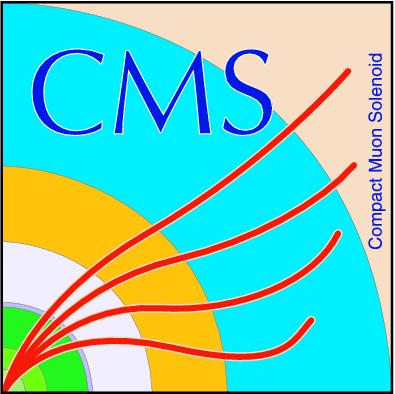
\includegraphics[width=1.5cm,keepaspectratio]{cmsLogo.jpeg}
}

\begin{document}
\renewcommand{\inserttotalframenumber}{\pageref{lastslide}}
\begin{frame}
\titlepage
\end{frame}

%\begin{frame}\frametitle{Table of contents}\tableofcontents
%\end{frame}
%%%%%%%%%%%%%%%%%%%%%%%%%%%%%%%%%%%%%%%%%%%%%%%%%%%%%%%%%%%%%%%%%%%%%%%%%%%%%%%%%%%%%%%%%%%%%%%%%%%%%%%
\section{Introduction}
%	\begin{frame}\frametitle{}	\end{frame}

%	\begin{frame}\frametitle{}	\begin{itemize}		\end{itemize}	\end{frame}

%	\begin{itemize}		\end{itemize}

%	\begin{block}{ }	\end{block}

%	\begin{columns}[t]	\column{.5\textwidth}	\column{.5\textwidth}	\end{columns}

%	\includegraphics[width=12cm,height=8cm]{}
%%%%%%%%%%%%%%%%%%%%%%%%%%%%%%%%%%%%%%%%%%%%%%%%%%%%%%%%%%%%%%%%%%%%%%%%%%%%%%%%%%%%%%%%%%%%%%%%%%%
%%%		Put figure one above other to point something in next click
%\begin{frame}\frametitle{Mass of Two tagged Jet }
%	 \begin{tikzpicture}[every node/.style={anchor=center}]
% 		\node(a) at (8,6){\includegraphics[width=12cm,height=7cm]{Massesjj.pdf}};
%		\pause
%		\node(b) at (10,7){\includegraphics[width=6cm]{Massesjj_zoomed.pdf}};
%		\draw[red,thick,->](8,8)--(3.5,6.5);
%	 \end{tikzpicture}
%\end{frame}
%%%%%%%%%%%%%%%%%%%%%%%%%%%%%%%%%%%%%%%%%%%%%%%%%%%%%%%%%%%%%%%%%%%%%%%%%%%%%%%%%%%%%%%%%%%%%%%%%%%
%%%%%%%%%%%%%%%%%%%%%%%%%%%%%%%%%%%%%%%%%%%%%
%	WRITE SOMETHING ON FIGURE
%\begin{tikzpicture}
%\draw (0, 0) node[inner sep=0] 
%{\includegraphics[width=12cm,height=9cm]{W_muon_pt.pdf}};
%\draw (2, 3) node {\color{red} Comment On Plot};
%\end{tikzpicture}
%%%%%%%%%%%%%%%%%%%%%%%%%%%%%%%%%%%%%%%%%%%%%
%%%%%%%%%%%%%%%%%%%%%%%%%%%%%%%%%%%%%%%%%%%%%
%\begin{frame}[shrink]\frametitle{Number of events after each applied cut}
%{\scriptsize \begin{tabular}{|p{1.5cm}|p{1cm}|c|c|c|c|c|}
%    	\hline
%	Sample & Total Event  & muon $p_T, \eta$ & pfMET & $Jet_{|\eta|}$ &  $Jet_{p_T}$  & $dR>0.5$\\
%	\hline
%	\hline
%	signal & 8 & 8 & 7 & 7  & 7 & 7\\
%	\hline
%	Data/mc & 0.6210 & 0.7379 & 0.7263 & 0.8272 & 0.8512 & 0.8512\\
%	\hline
%\end{tabular}
%}
%\end{frame}
%%%%%%%%%%%%%%%%%%%%%%%%%%%%%%%%%%%%%%%%%%%%

\section{Figures}
% Pointer-rk
\begin{frame}\frametitle{Tracker Hit position 1187}
%        \begin{tikzpicture}
%         \draw (0, 0) node[inner sep=0]
 %        {
	 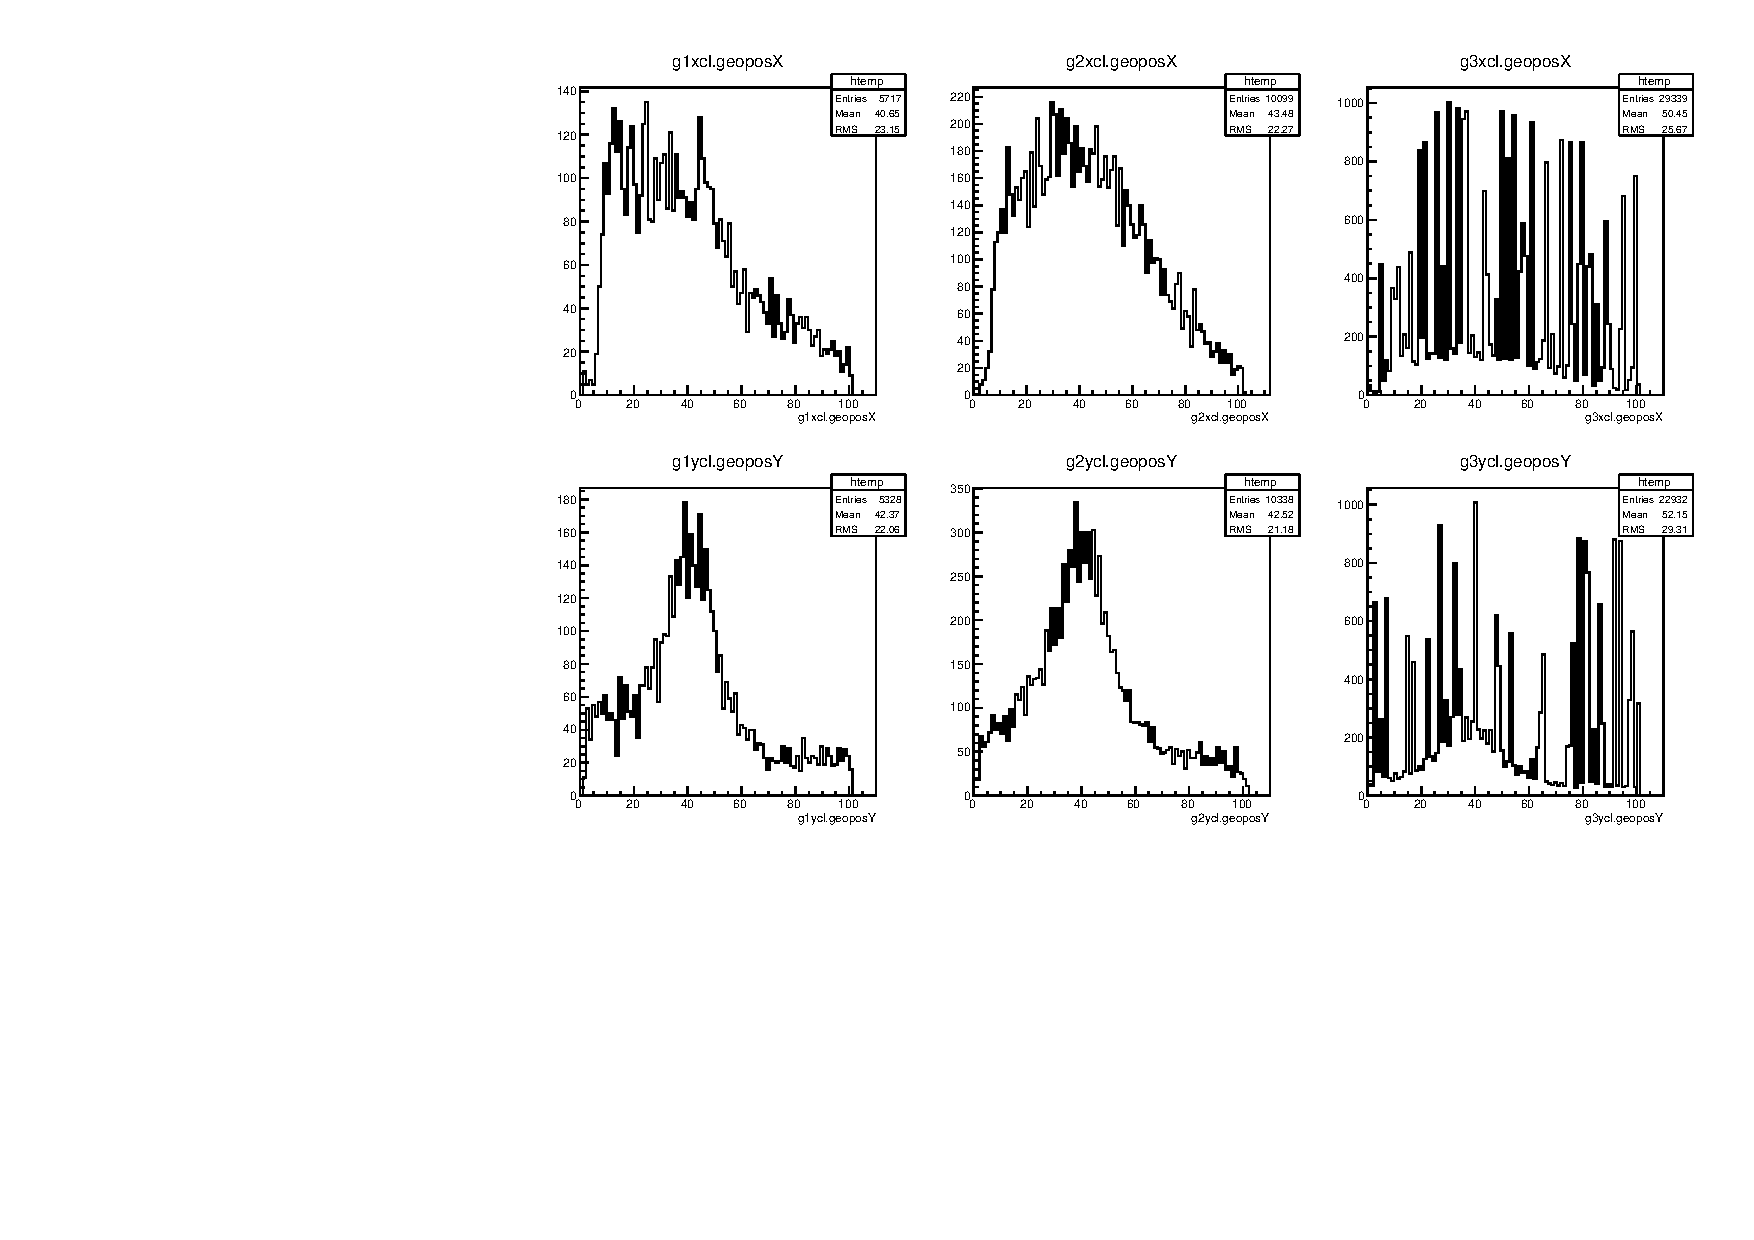
\includegraphics[width=12cm,height=8cm]{Tracker_Hit_position_1187.pdf}
%         };
%         \draw (2, 3) node {\color{red} };	% can comment anyting at a position 2,3
%         \end{tikzpicture}
\end{frame}
\begin{frame}\frametitle{Tracker Hit position 1184}
%        \begin{tikzpicture}
%         \draw (0, 0) node[inner sep=0]
 %        {
	 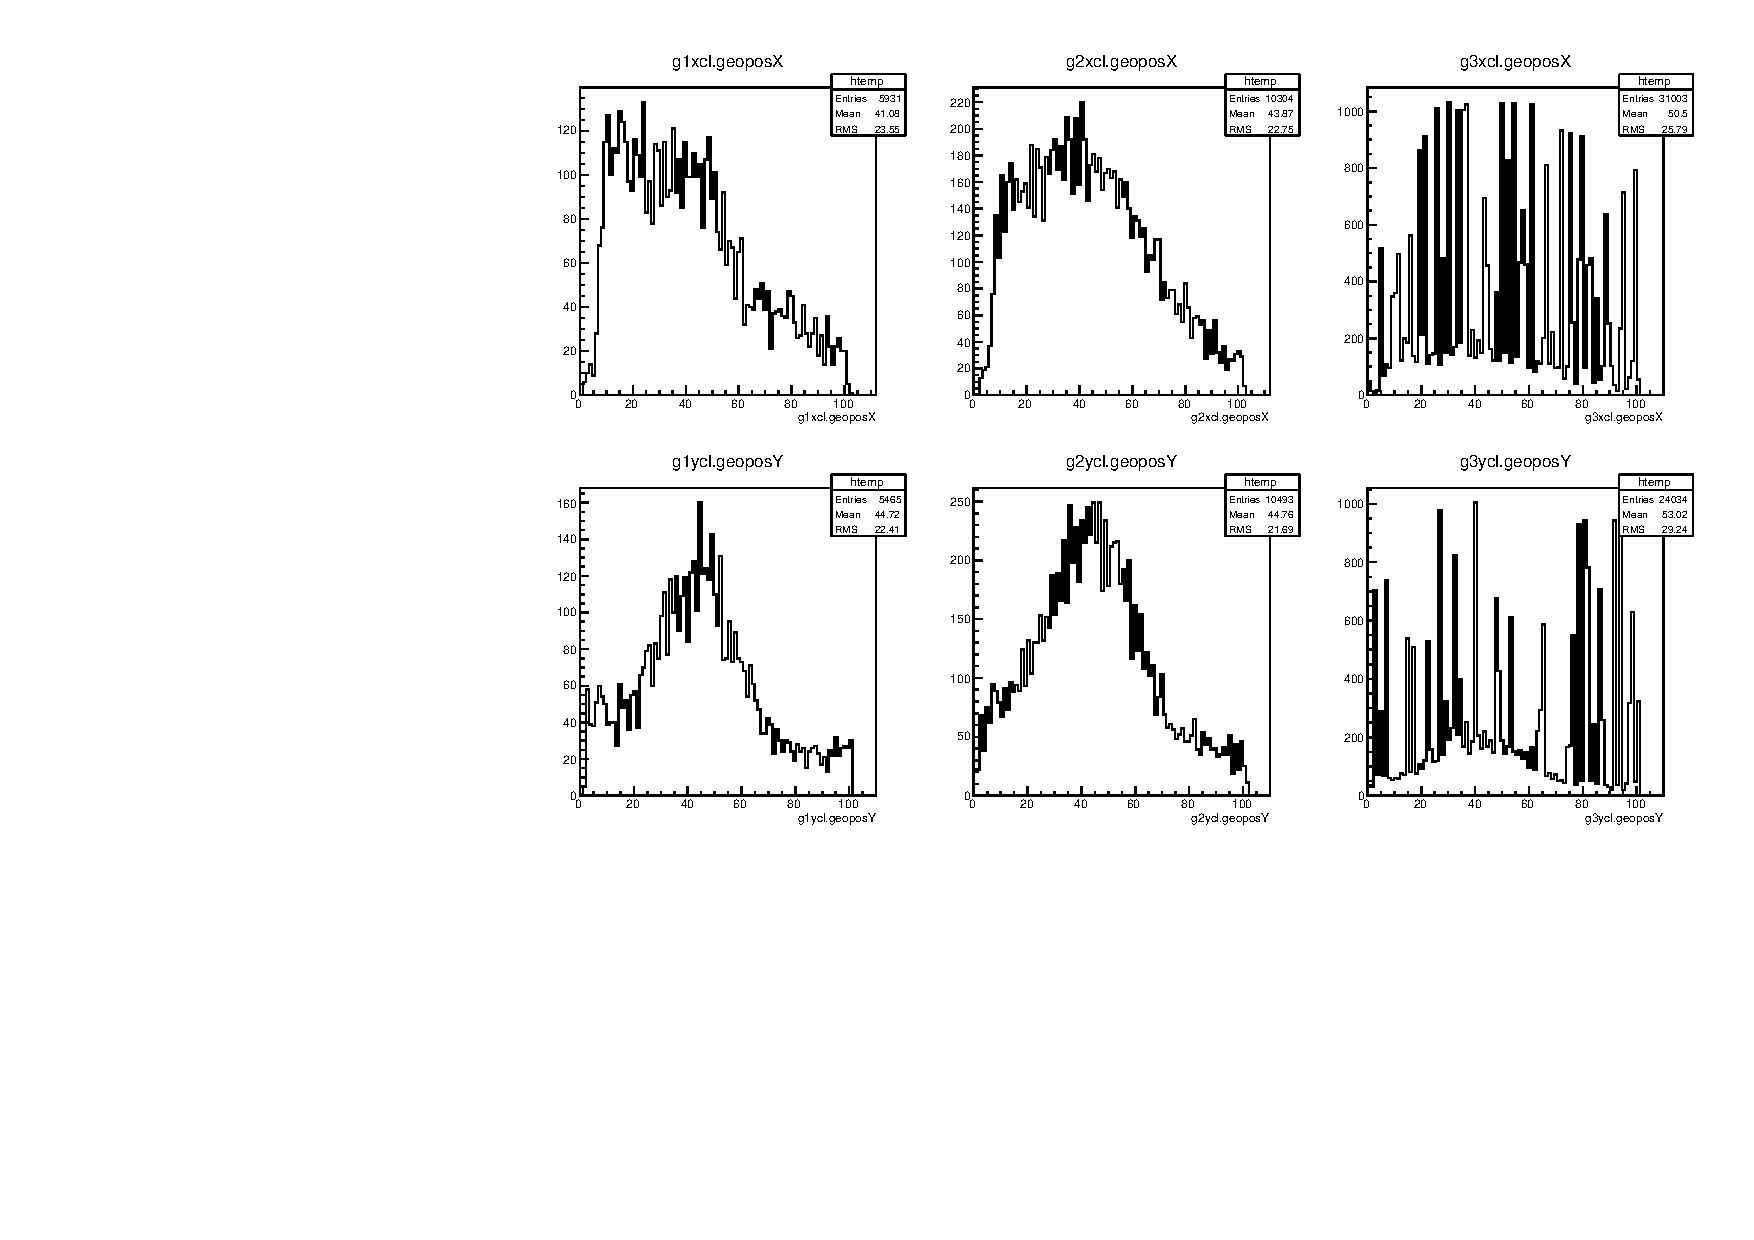
\includegraphics[width=12cm,height=8cm]{Tracker_Hit_position_1184.pdf}
%         };
%         \draw (2, 3) node {\color{red} };	% can comment anyting at a position 2,3
%         \end{tikzpicture}
\end{frame}
\begin{frame}\frametitle{Tracker Hit position 1183}
%        \begin{tikzpicture}
%         \draw (0, 0) node[inner sep=0]
 %        {
	 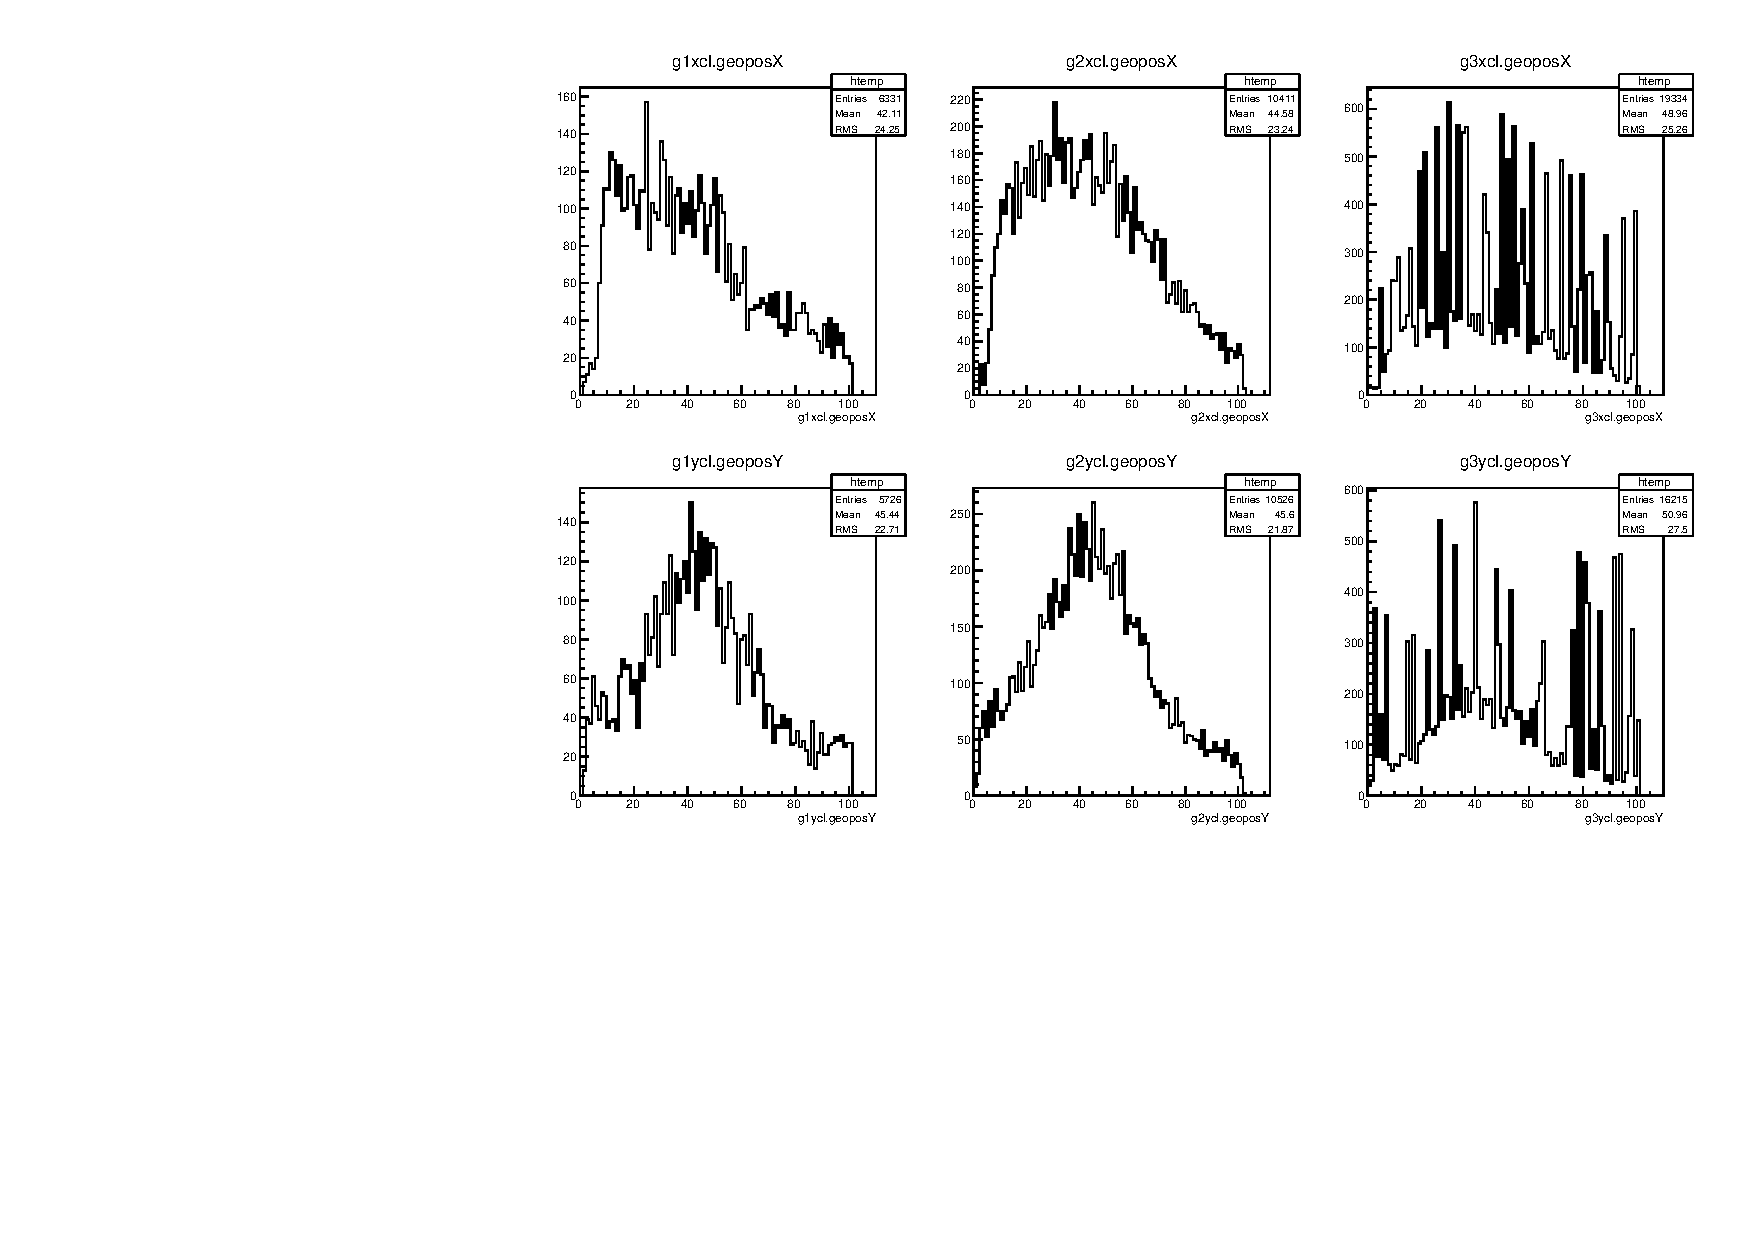
\includegraphics[width=12cm,height=8cm]{Tracker_Hit_position_1183.pdf}
%         };
%         \draw (2, 3) node {\color{red} };	% can comment anyting at a position 2,3
%         \end{tikzpicture}
\end{frame}
\begin{frame}\frametitle{Tracker Hit position 1182}
%        \begin{tikzpicture}
%         \draw (0, 0) node[inner sep=0]
 %        {
	 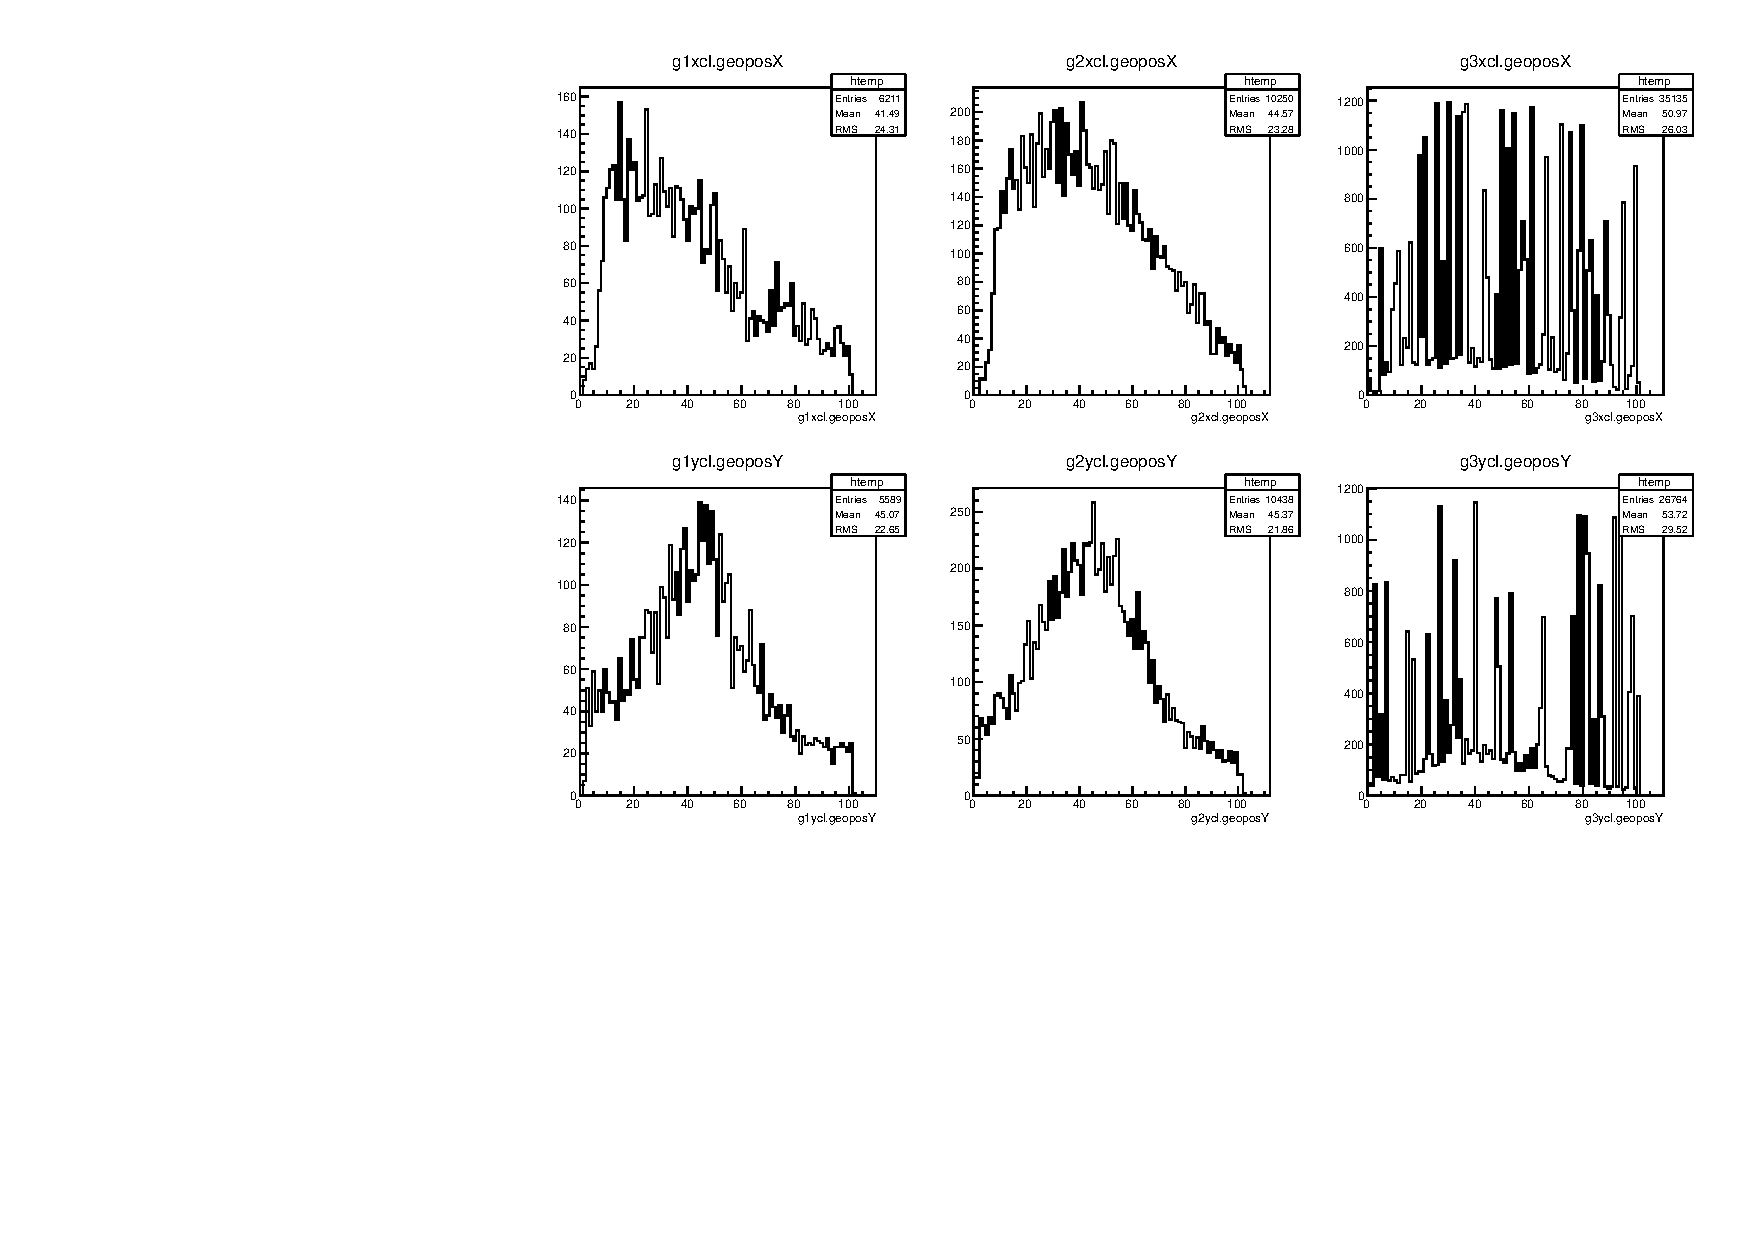
\includegraphics[width=12cm,height=8cm]{Tracker_Hit_position_1182.pdf}
%         };
%         \draw (2, 3) node {\color{red} };	% can comment anyting at a position 2,3
%         \end{tikzpicture}
\end{frame}
\begin{frame}\frametitle{Tracker Hit position 1181}
%        \begin{tikzpicture}
%         \draw (0, 0) node[inner sep=0]
 %        {
	 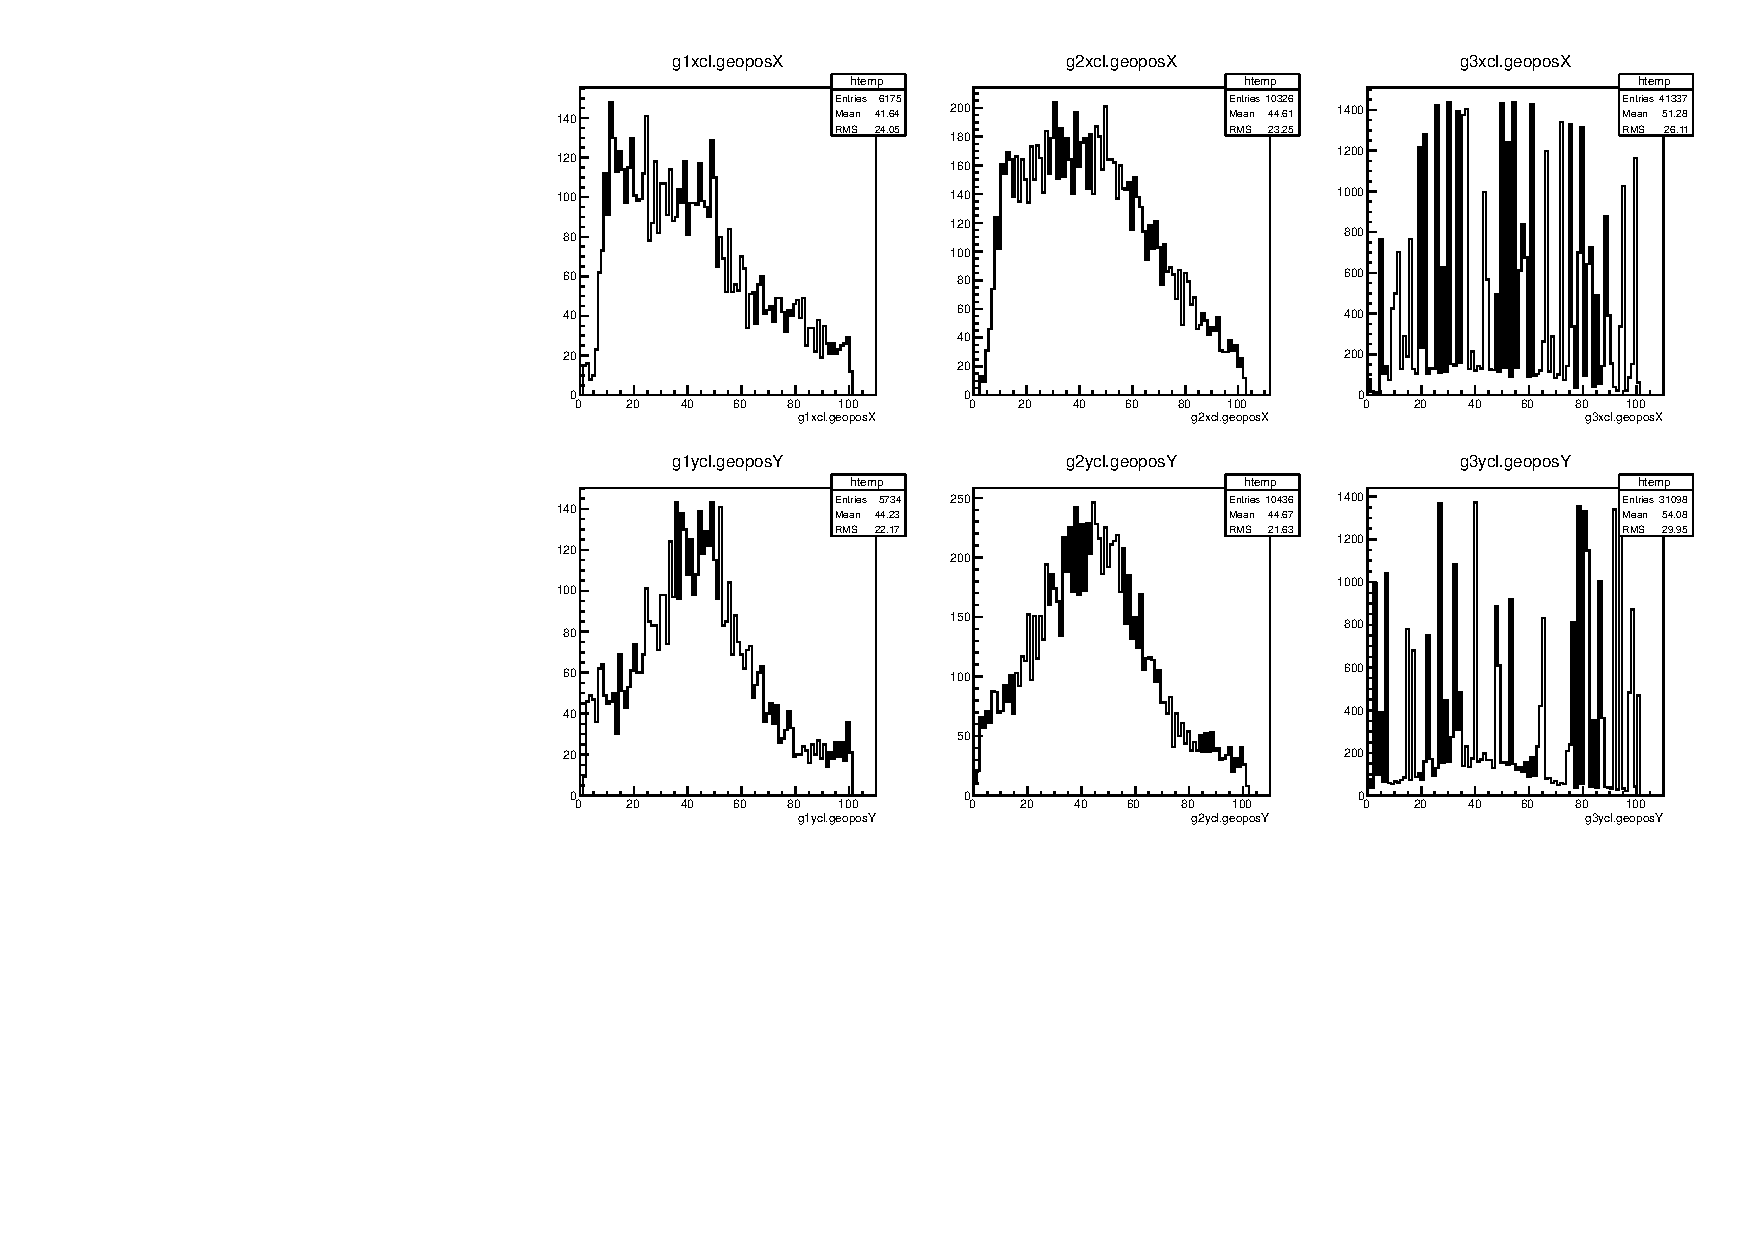
\includegraphics[width=12cm,height=8cm]{Tracker_Hit_position_1181.pdf}
%         };
%         \draw (2, 3) node {\color{red} };	% can comment anyting at a position 2,3
%         \end{tikzpicture}
\end{frame}
\begin{frame}\frametitle{Tracker Hit position 1180}
%        \begin{tikzpicture}
%         \draw (0, 0) node[inner sep=0]
 %        {
	 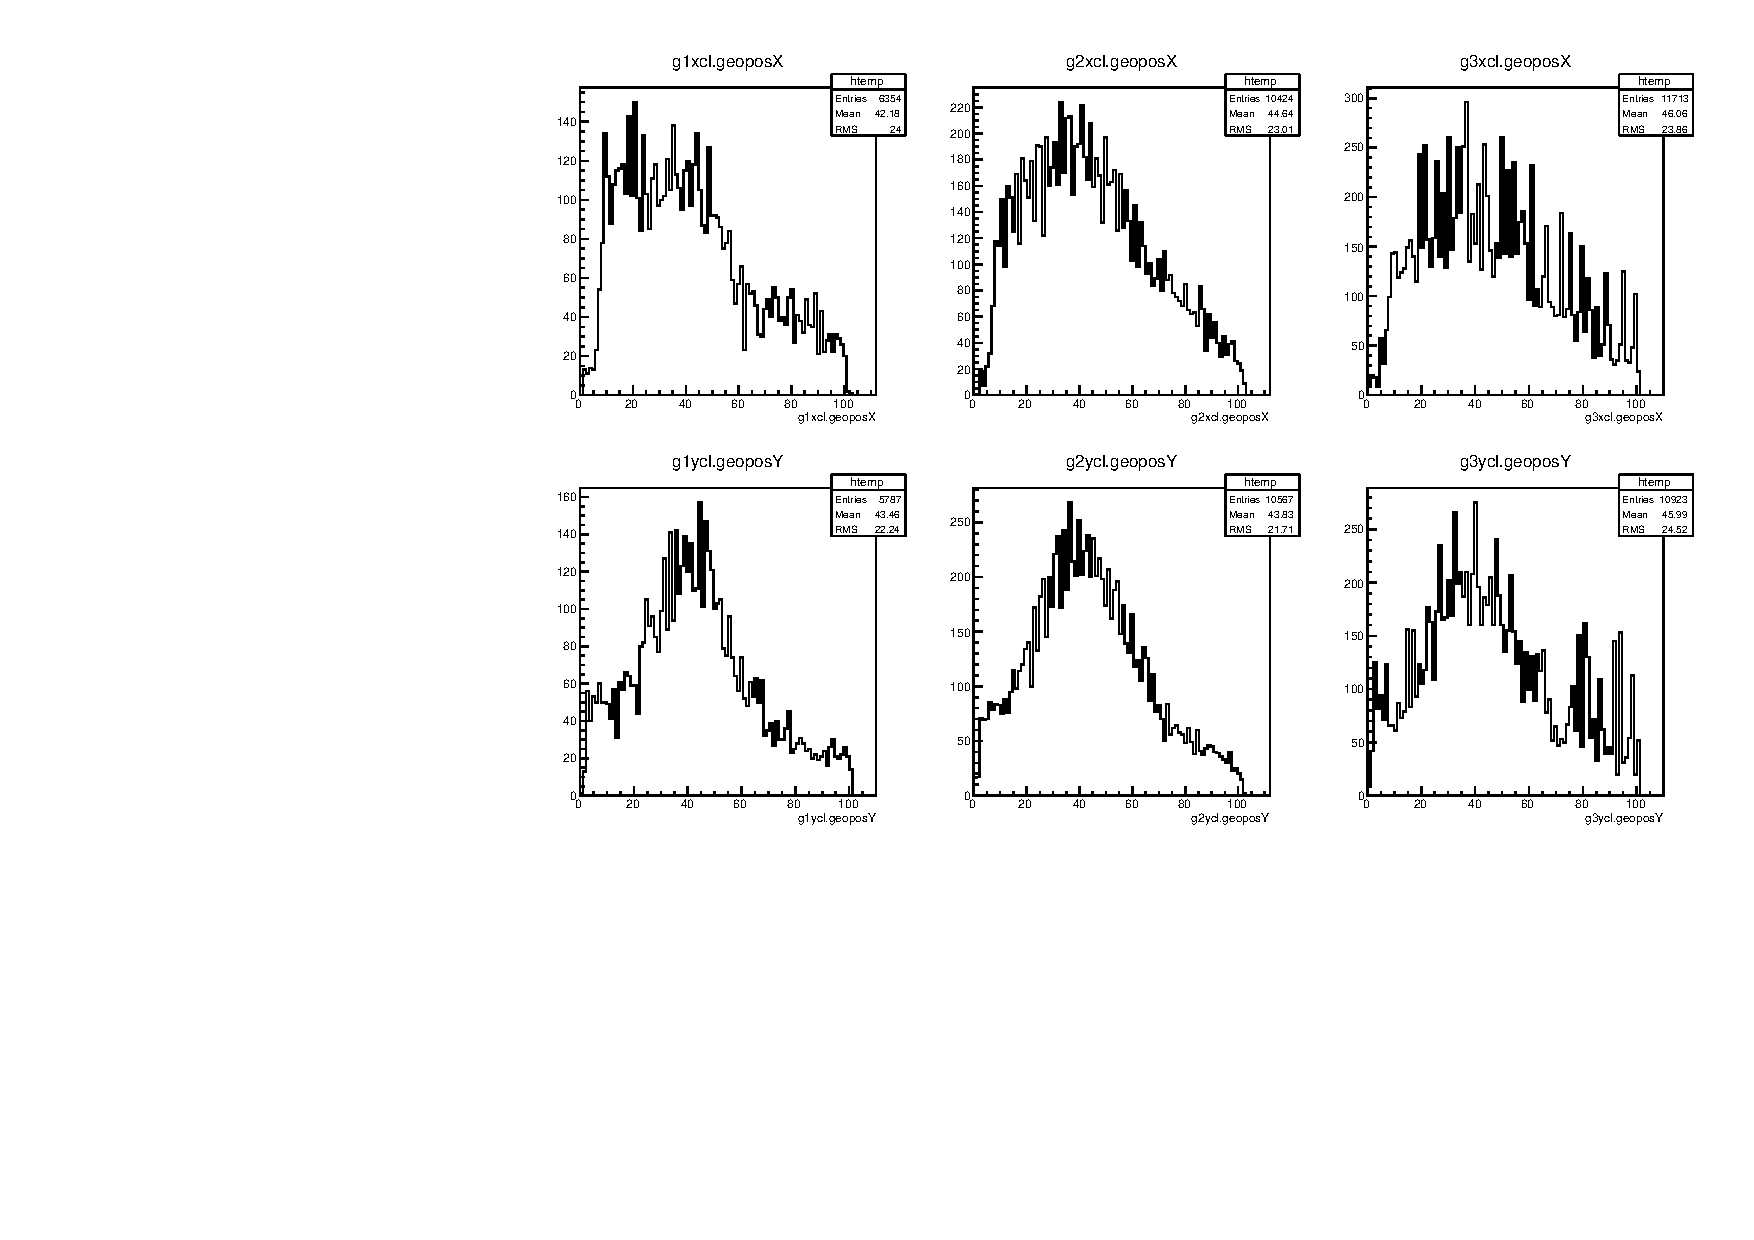
\includegraphics[width=12cm,height=8cm]{Tracker_Hit_position_1180.pdf}
%         };
%         \draw (2, 3) node {\color{red} };	% can comment anyting at a position 2,3
%         \end{tikzpicture}
\end{frame}
\begin{frame}\frametitle{Tracker Hit position 1179}
%        \begin{tikzpicture}
%         \draw (0, 0) node[inner sep=0]
 %        {
	 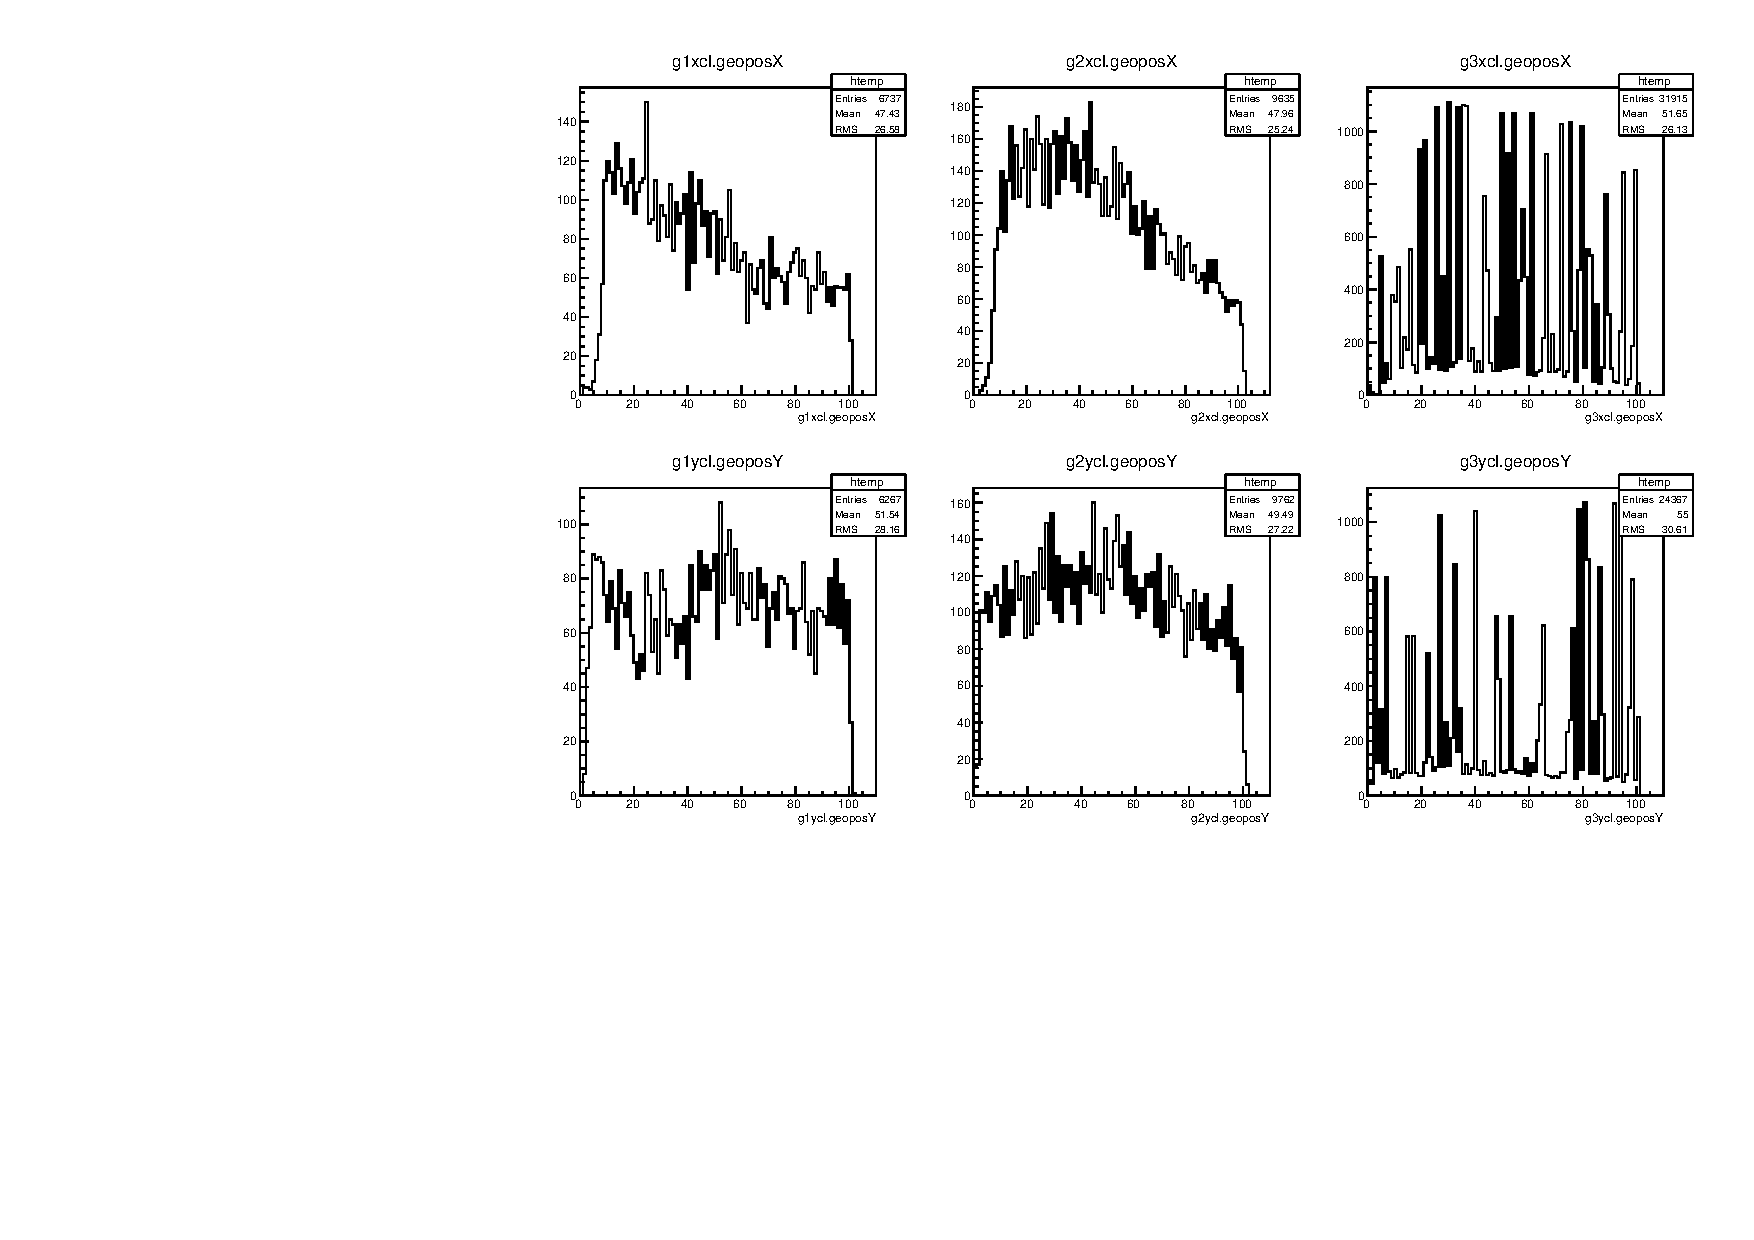
\includegraphics[width=12cm,height=8cm]{Tracker_Hit_position_1179.pdf}
%         };
%         \draw (2, 3) node {\color{red} };	% can comment anyting at a position 2,3
%         \end{tikzpicture}
\end{frame}
\begin{frame}\frametitle{Tracker Hit position 1178}
%        \begin{tikzpicture}
%         \draw (0, 0) node[inner sep=0]
 %        {
	 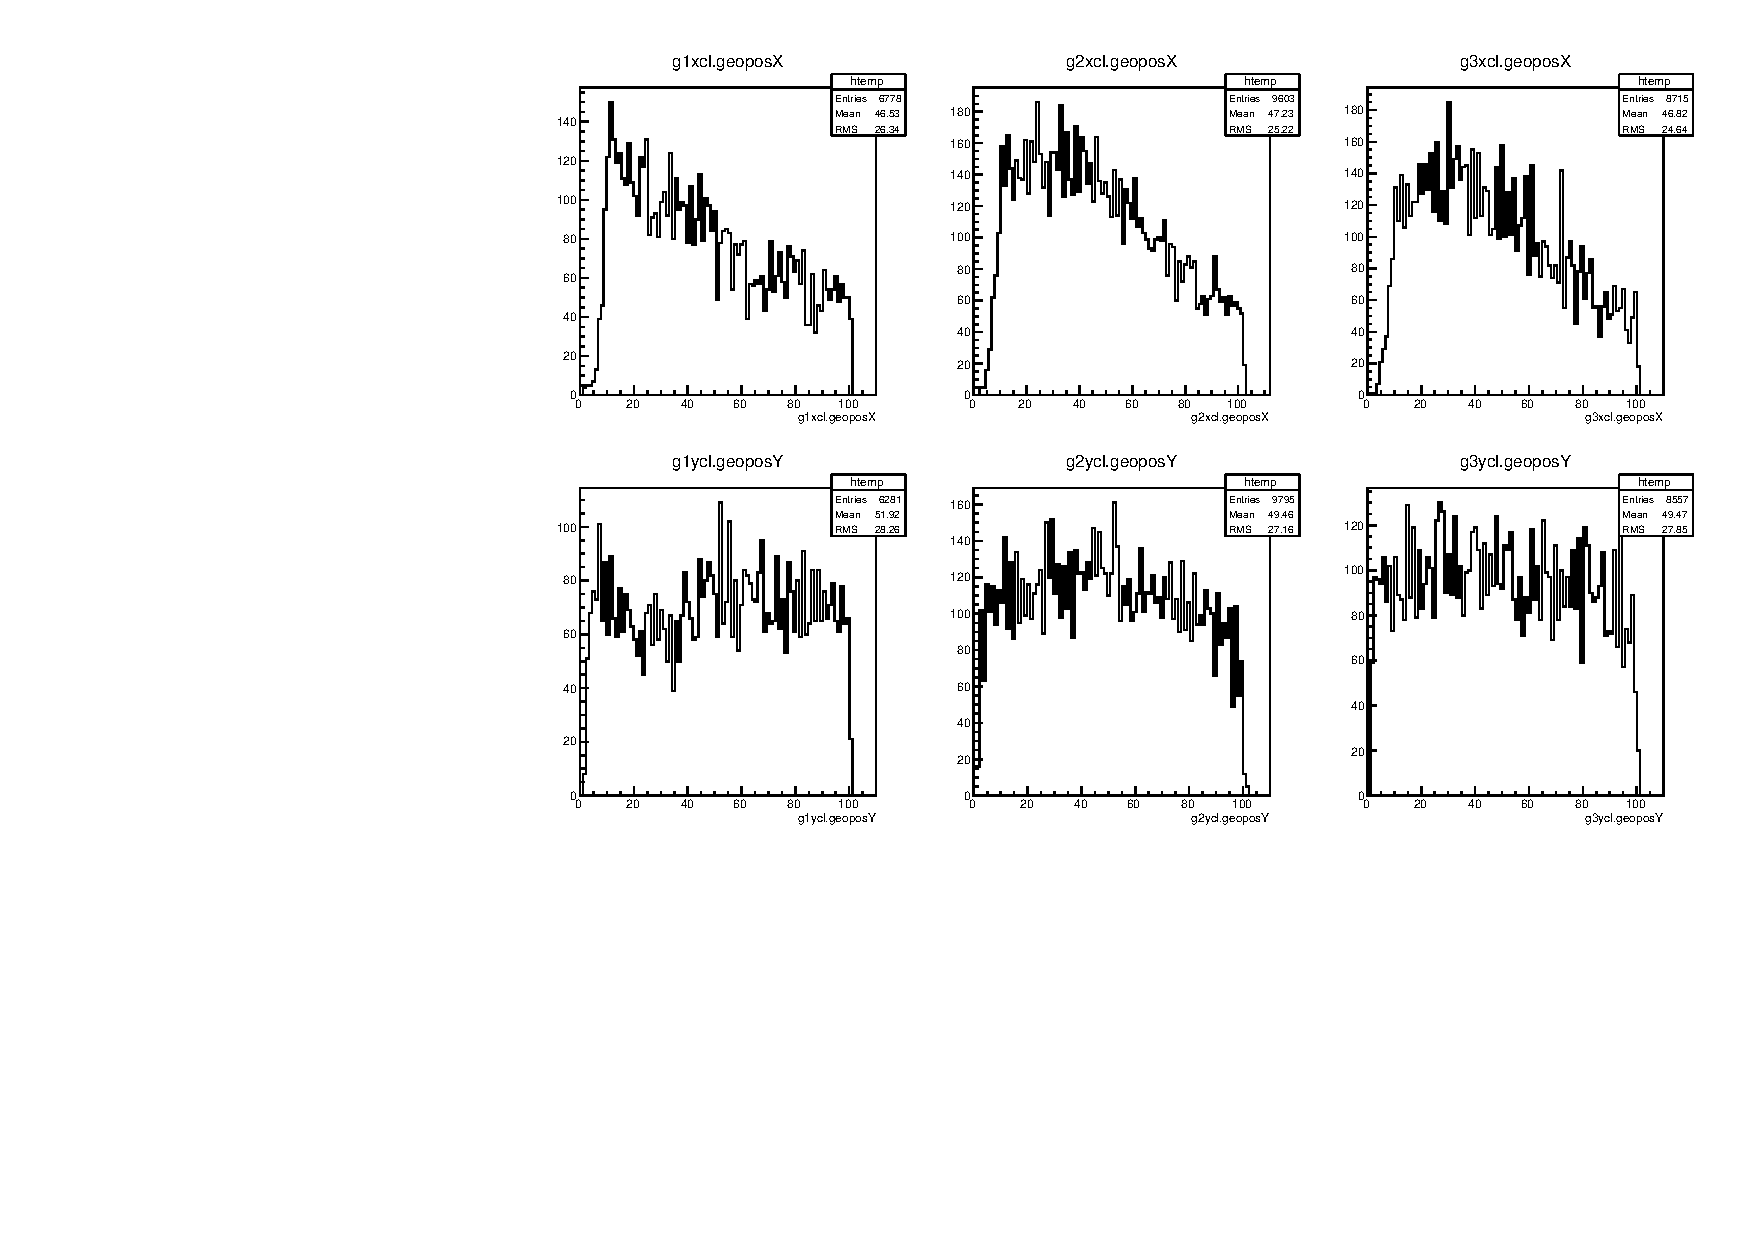
\includegraphics[width=12cm,height=8cm]{Tracker_Hit_position_1178.pdf}
%         };
%         \draw (2, 3) node {\color{red} };	% can comment anyting at a position 2,3
%         \end{tikzpicture}
\end{frame}
\begin{frame}\frametitle{Tracker Hit position 1174}
%        \begin{tikzpicture}
%         \draw (0, 0) node[inner sep=0]
 %        {
	 
\includegraphics[width=12cm,height=8cm]{Tracker_Hit_position_1174.pdf}
%         };
%         \draw (2, 3) node {\color{red} };	% can comment anyting at a position 2,3
%         \end{tikzpicture}
\end{frame}
\begin{frame}\frametitle{Tracker Hit position 1173}
%        \begin{tikzpicture}
%         \draw (0, 0) node[inner sep=0]
 %        {
	 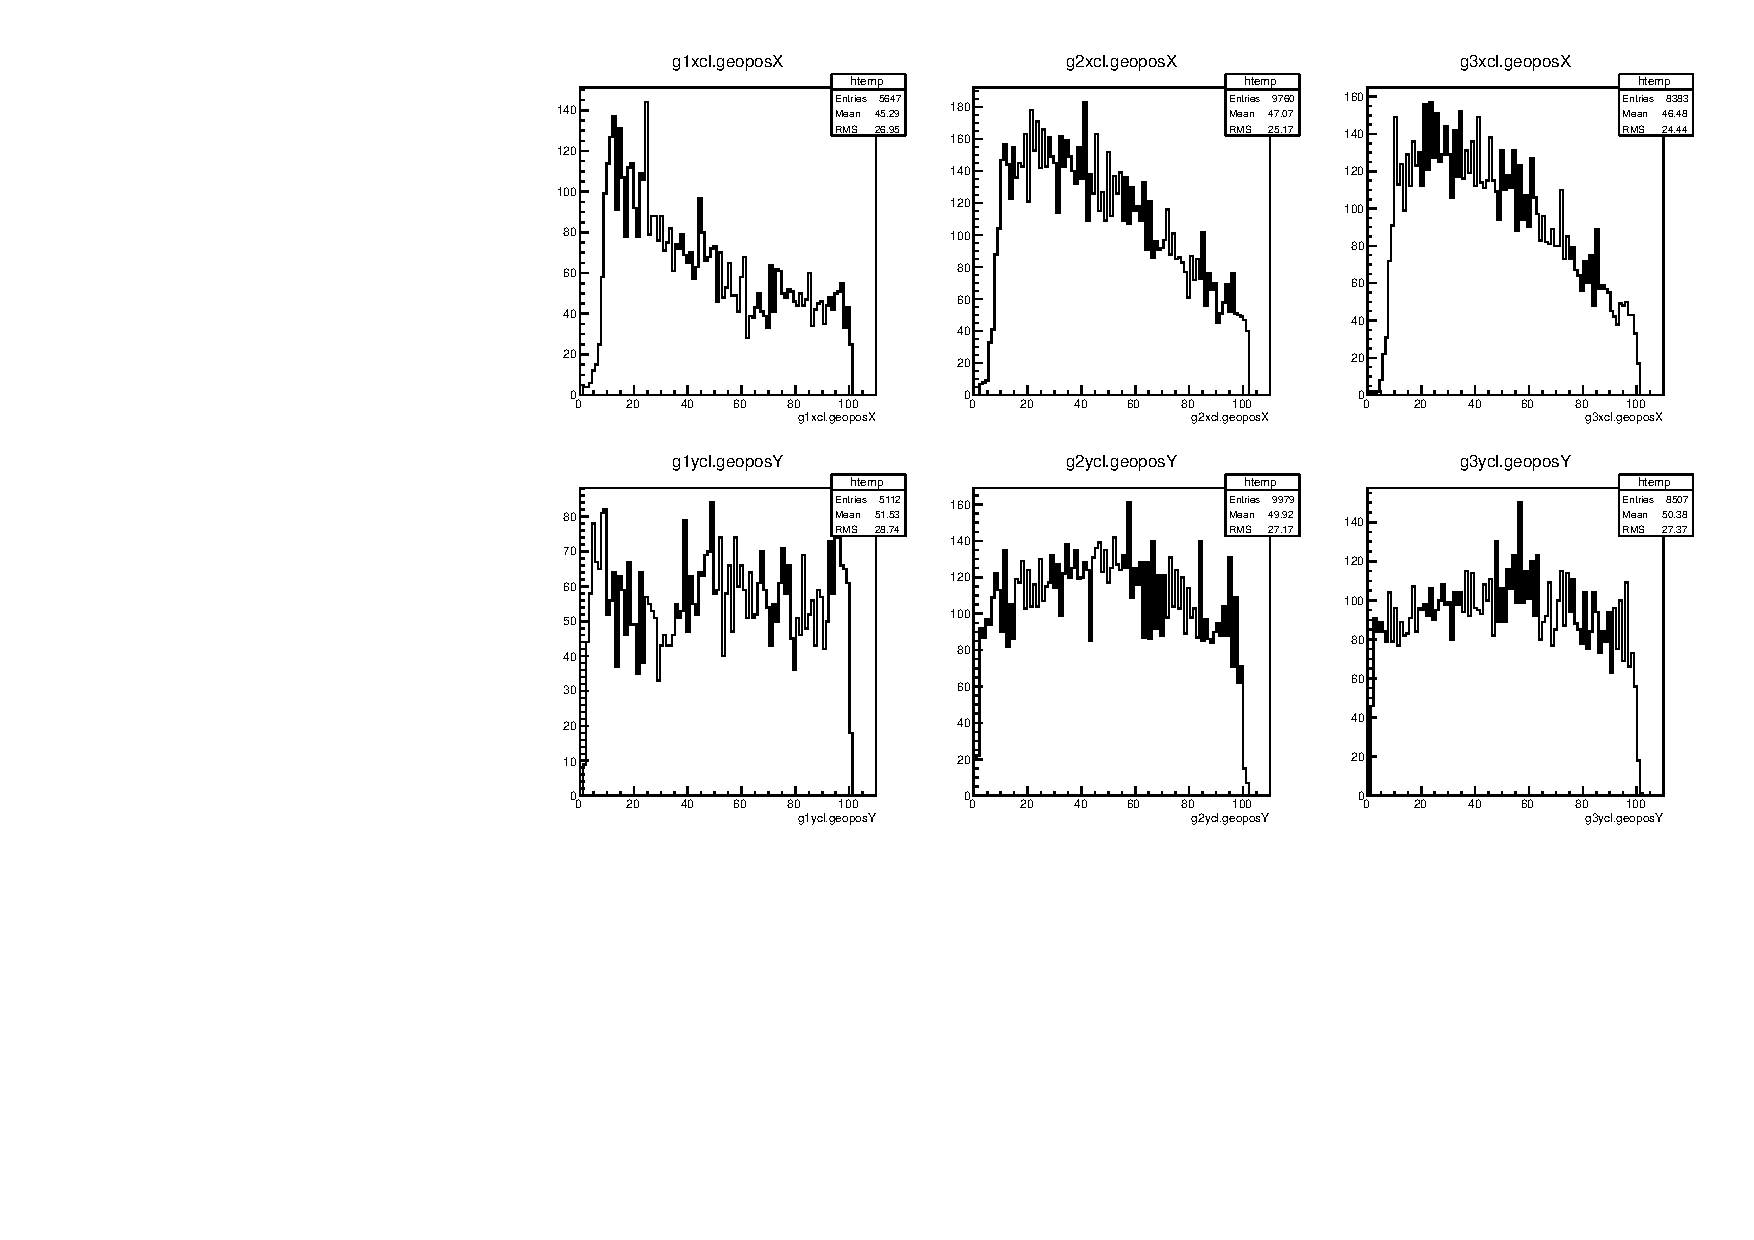
\includegraphics[width=12cm,height=8cm]{Tracker_Hit_position_1173.pdf}
%         };
%         \draw (2, 3) node {\color{red} };	% can comment anyting at a position 2,3
%         \end{tikzpicture}
\end{frame}
\begin{frame}\frametitle{Tracker Hit position 1172}
%        \begin{tikzpicture}
%         \draw (0, 0) node[inner sep=0]
 %        {
	 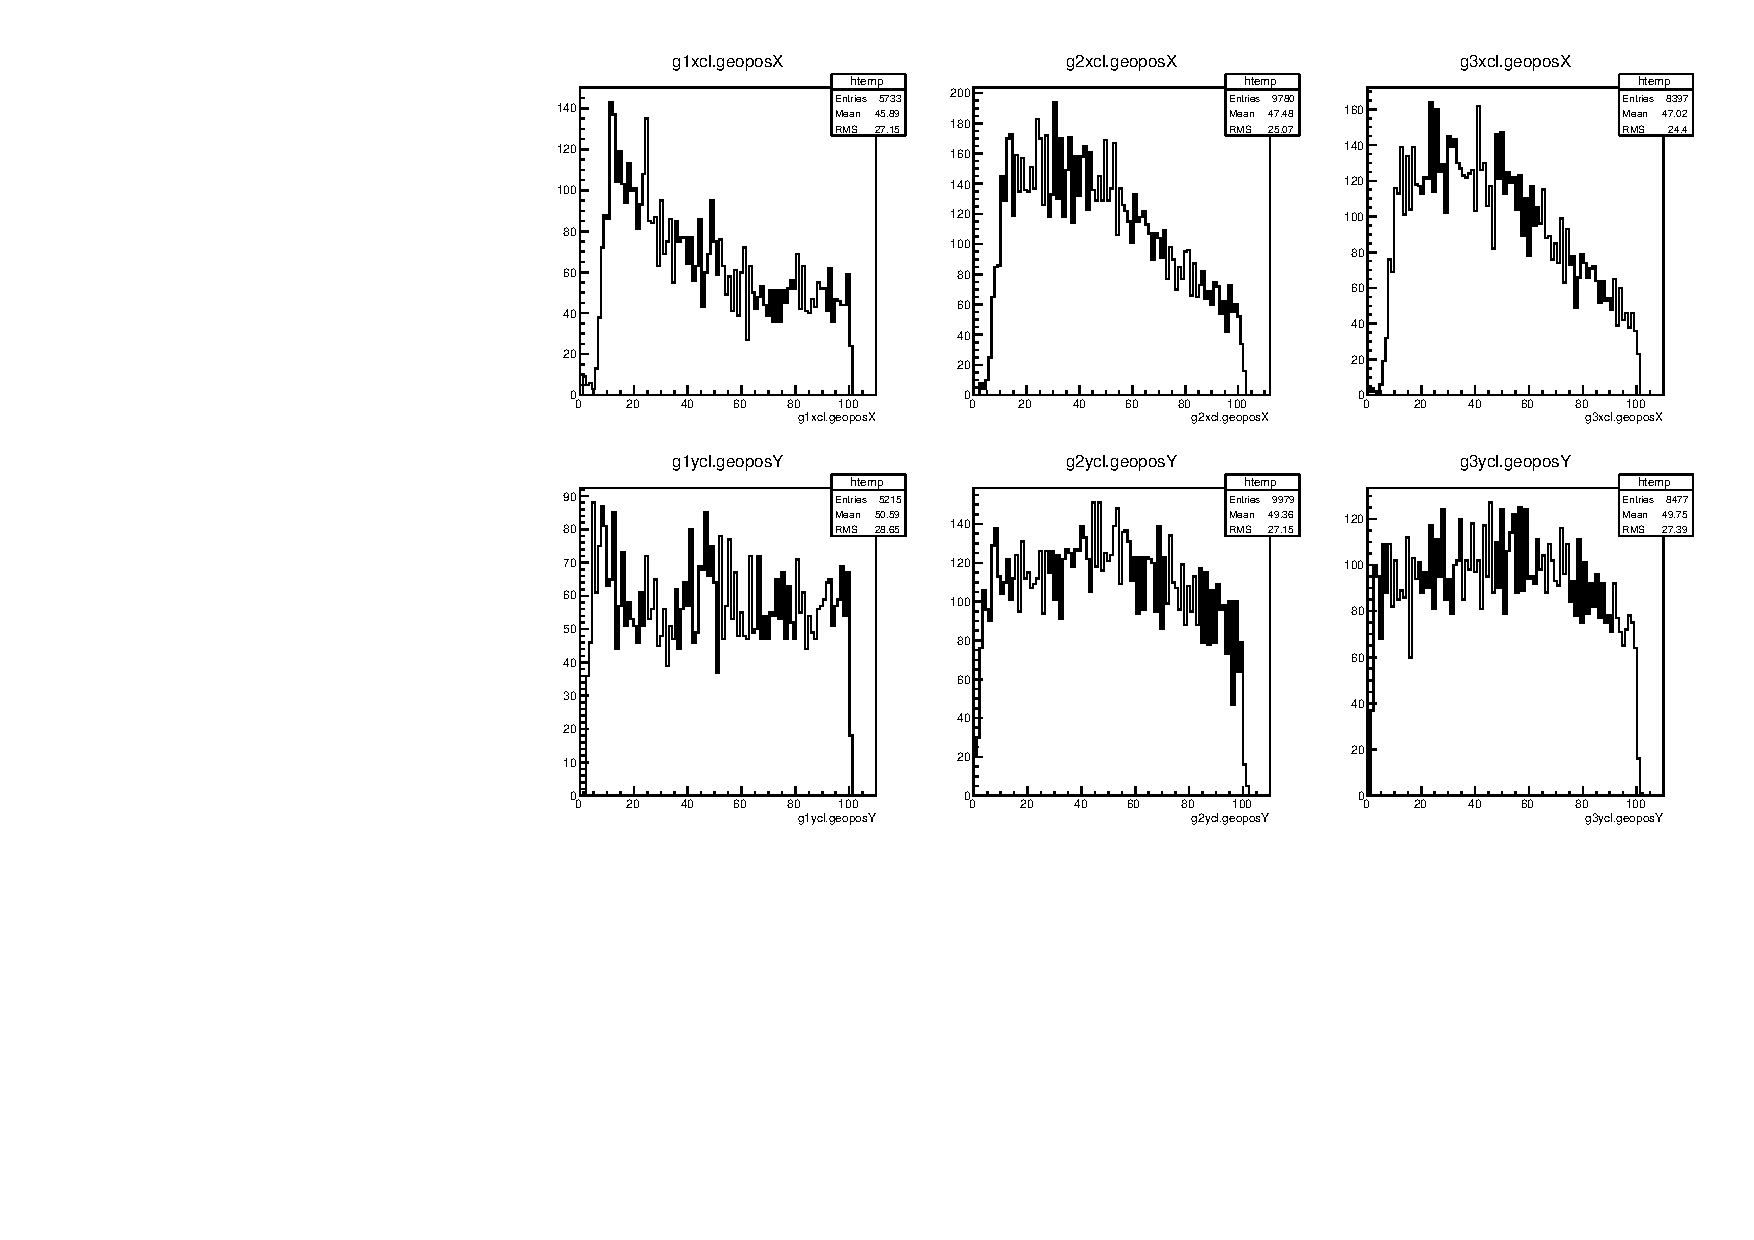
\includegraphics[width=12cm,height=8cm]{Tracker_Hit_position_1172.pdf}
%         };
%         \draw (2, 3) node {\color{red} };	% can comment anyting at a position 2,3
%         \end{tikzpicture}
\end{frame}
\begin{frame}\frametitle{Tracker Hit position 1170}
%        \begin{tikzpicture}
%         \draw (0, 0) node[inner sep=0]
 %        {
	 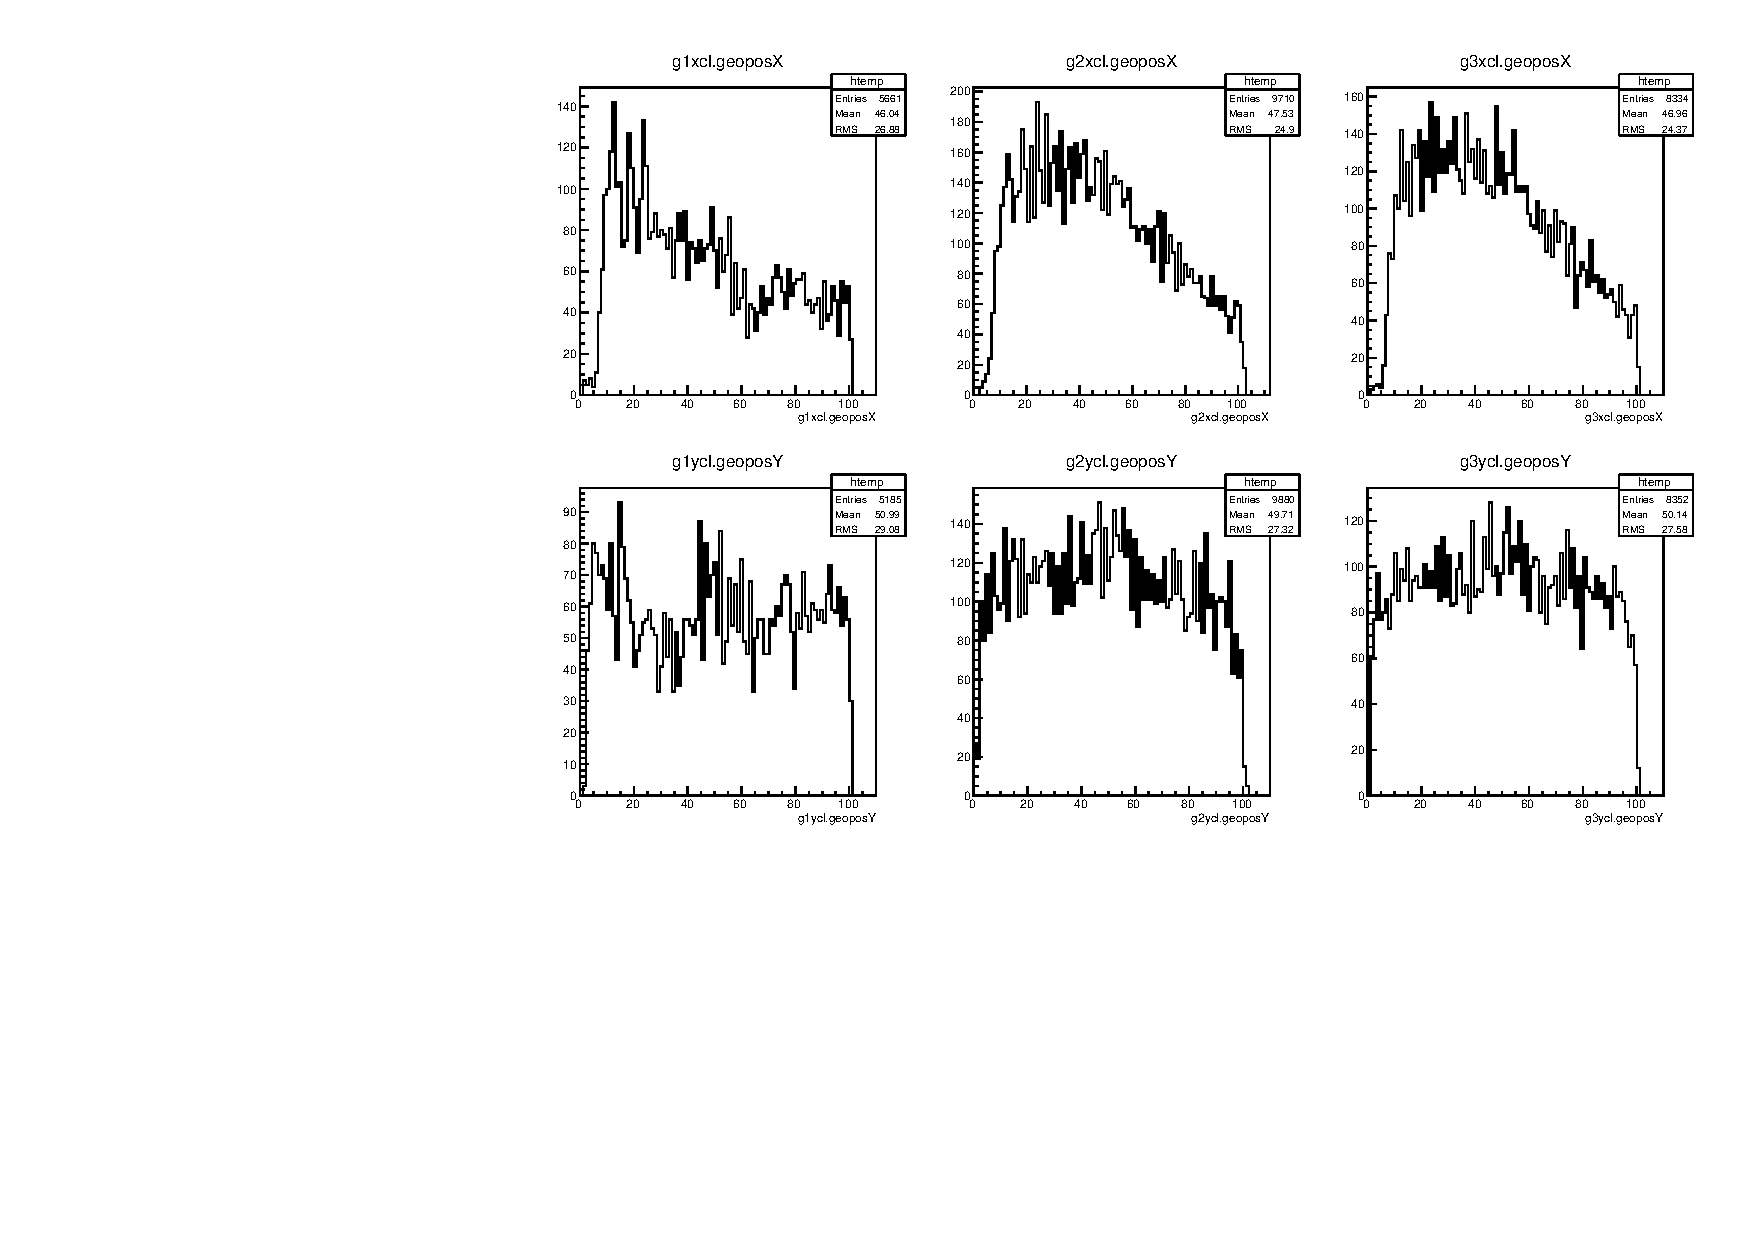
\includegraphics[width=12cm,height=8cm]{Tracker_Hit_position_1170.pdf}
%         };
%         \draw (2, 3) node {\color{red} };	% can comment anyting at a position 2,3
%         \end{tikzpicture}
\end{frame}
\begin{frame}\frametitle{Tracker Hit position 1168}
%        \begin{tikzpicture}
%         \draw (0, 0) node[inner sep=0]
 %        {
	 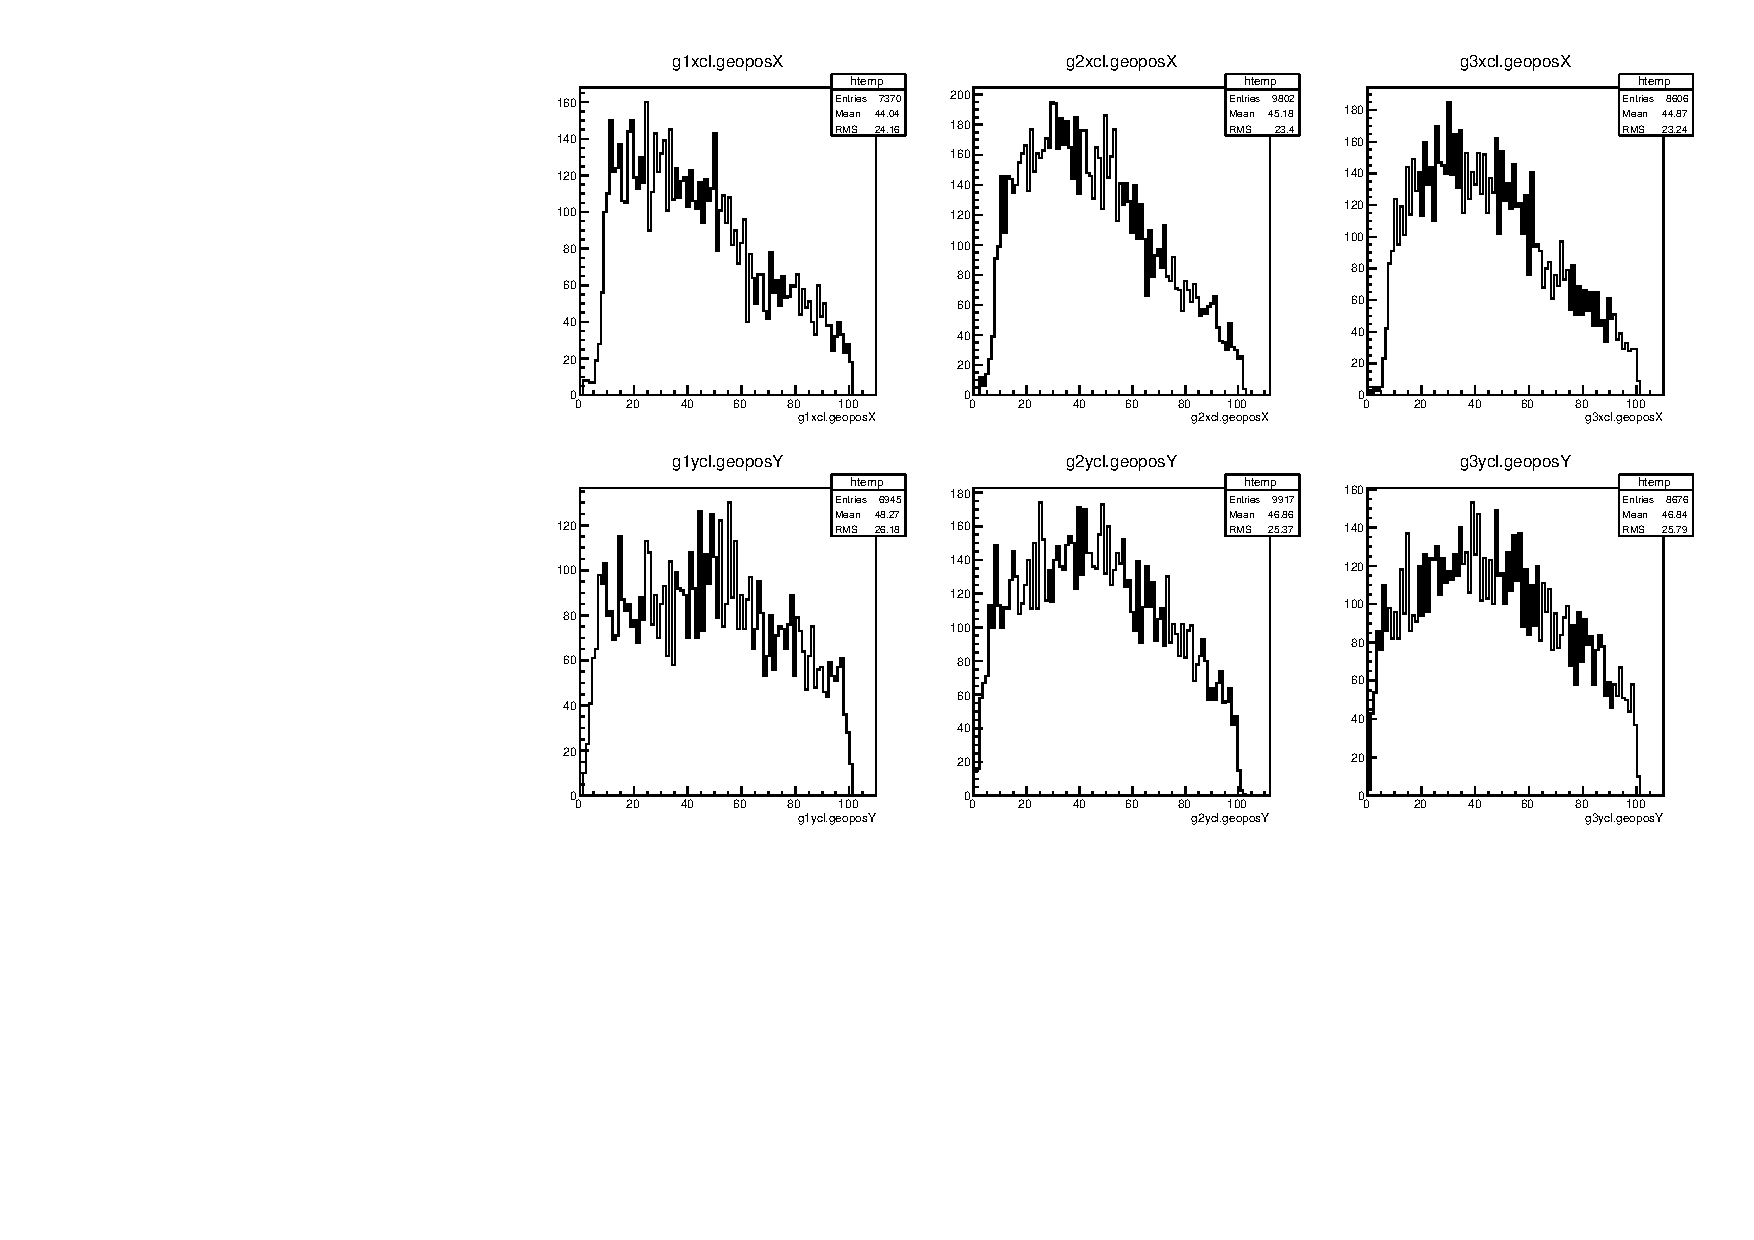
\includegraphics[width=12cm,height=8cm]{Tracker_Hit_position_1168.pdf}
%         };
%         \draw (2, 3) node {\color{red} };	% can comment anyting at a position 2,3
%         \end{tikzpicture}
\end{frame}
\begin{frame}\frametitle{Tracker Hit position 1167}
%        \begin{tikzpicture}
%         \draw (0, 0) node[inner sep=0]
 %        {
	 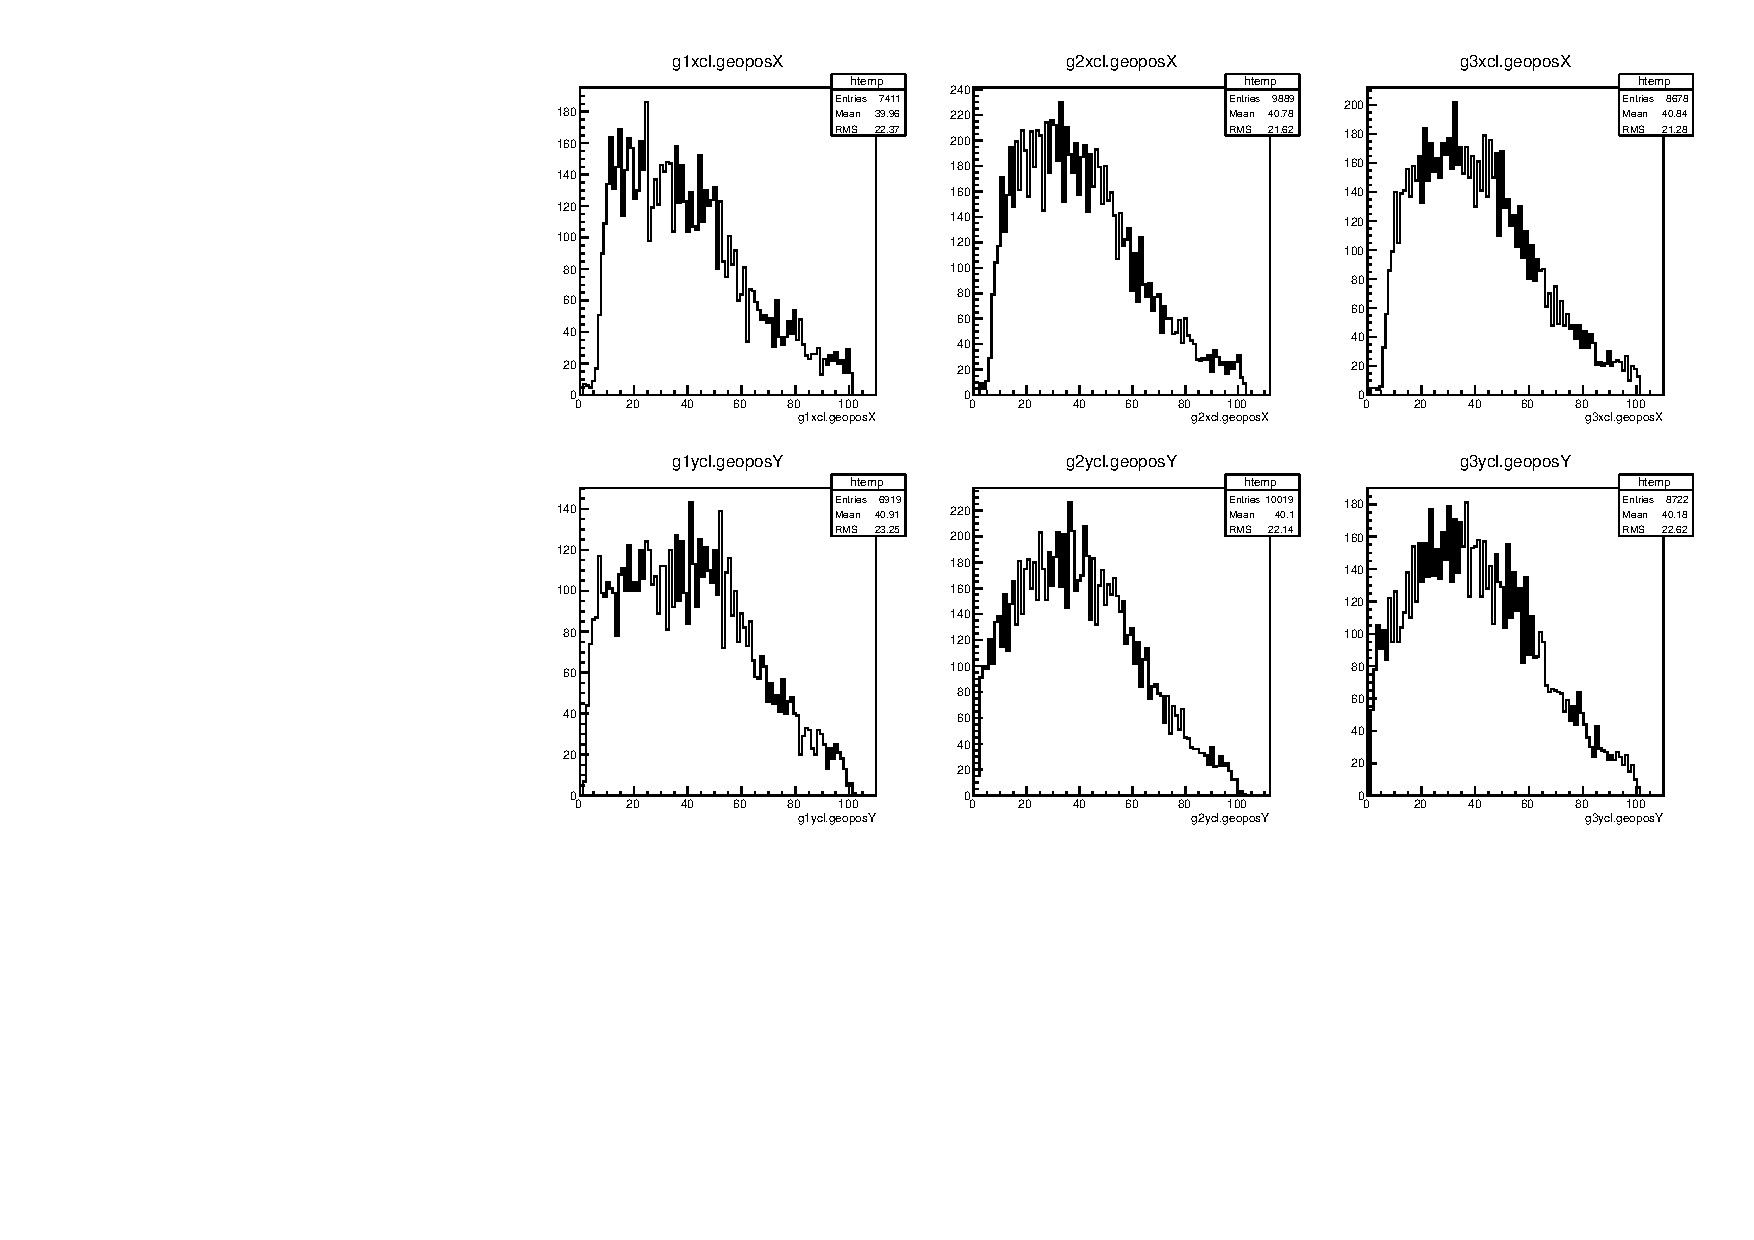
\includegraphics[width=12cm,height=8cm]{Tracker_Hit_position_1167.pdf}
%         };
%         \draw (2, 3) node {\color{red} };	% can comment anyting at a position 2,3
%         \end{tikzpicture}
\end{frame}
\begin{frame}\frametitle{Tracker Hit position 1166}
%        \begin{tikzpicture}
%         \draw (0, 0) node[inner sep=0]
 %        {
	 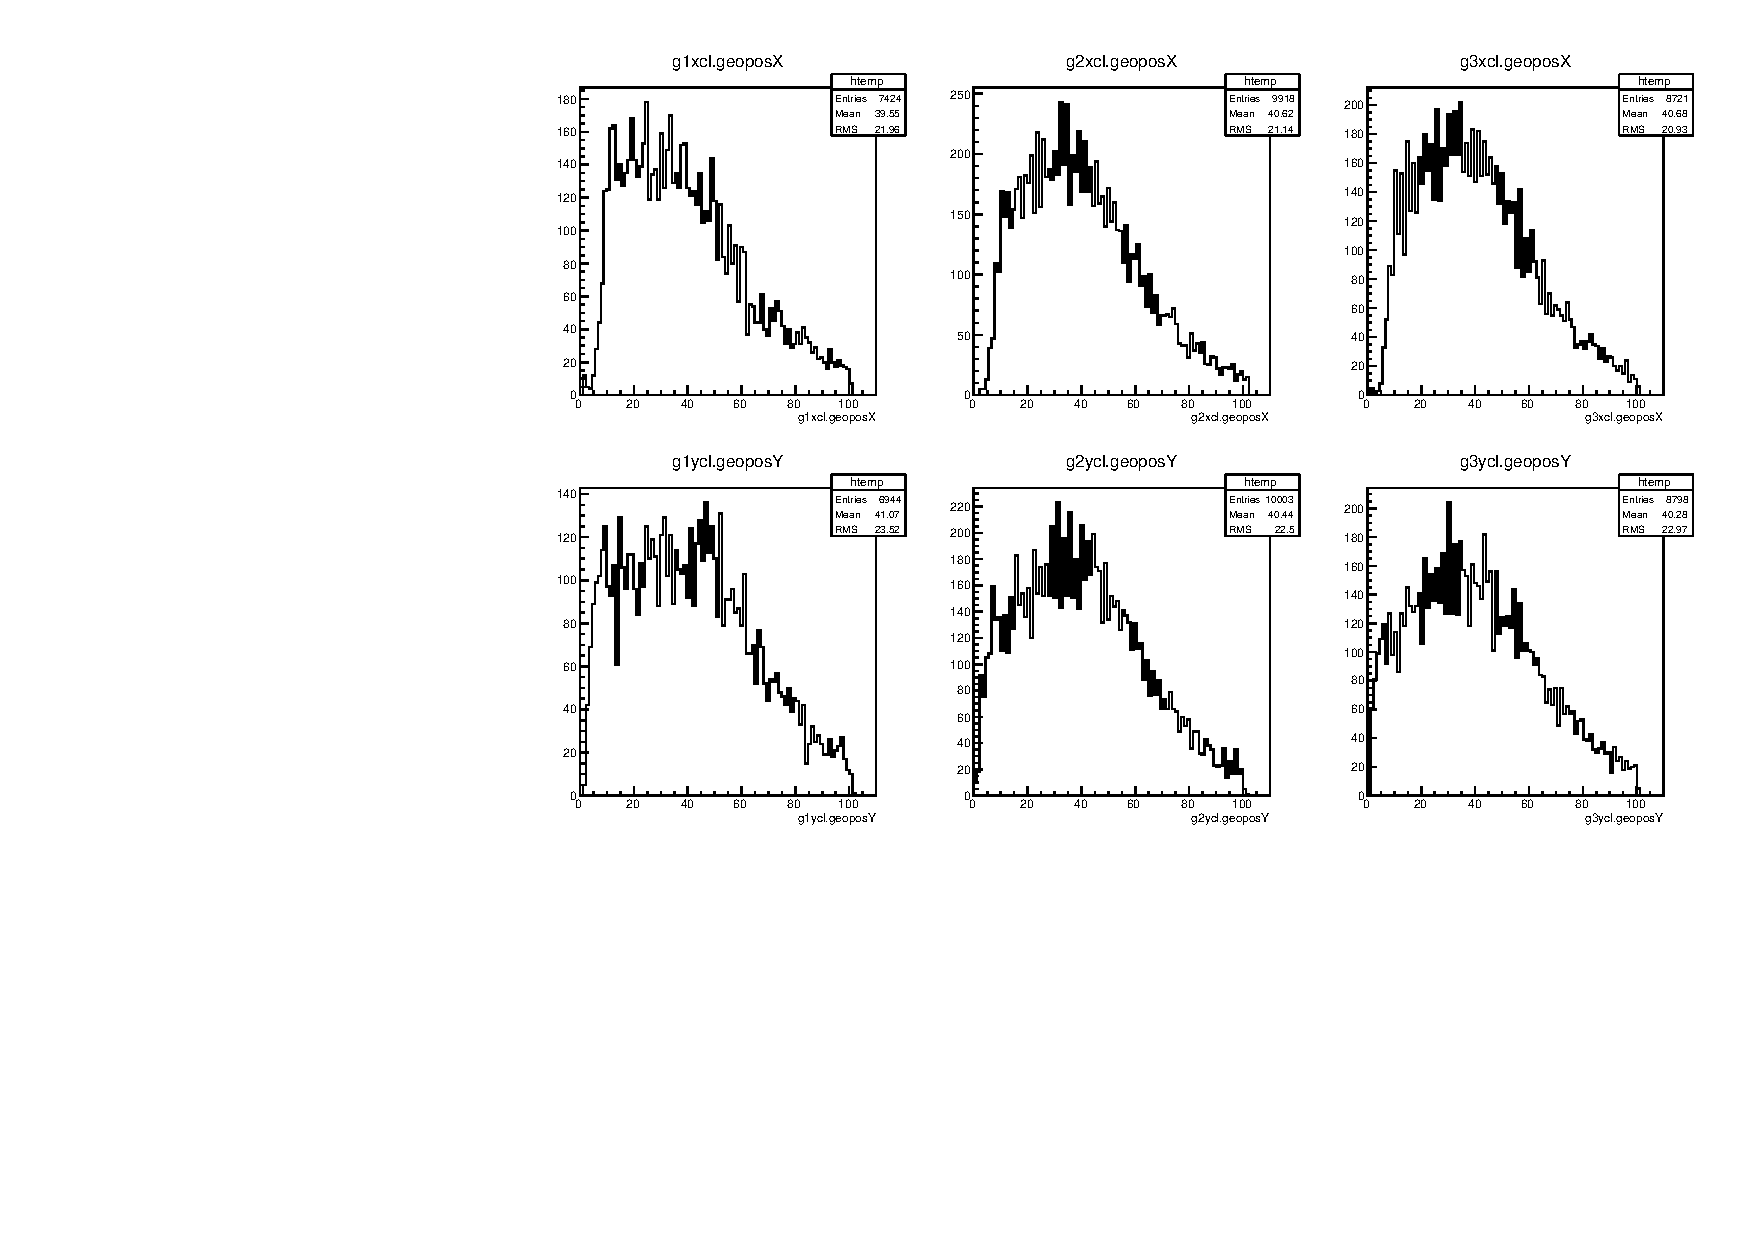
\includegraphics[width=12cm,height=8cm]{Tracker_Hit_position_1166.pdf}
%         };
%         \draw (2, 3) node {\color{red} };	% can comment anyting at a position 2,3
%         \end{tikzpicture}
\end{frame}
\begin{frame}\frametitle{Tracker Hit position 1165}
%        \begin{tikzpicture}
%         \draw (0, 0) node[inner sep=0]
 %        {
	 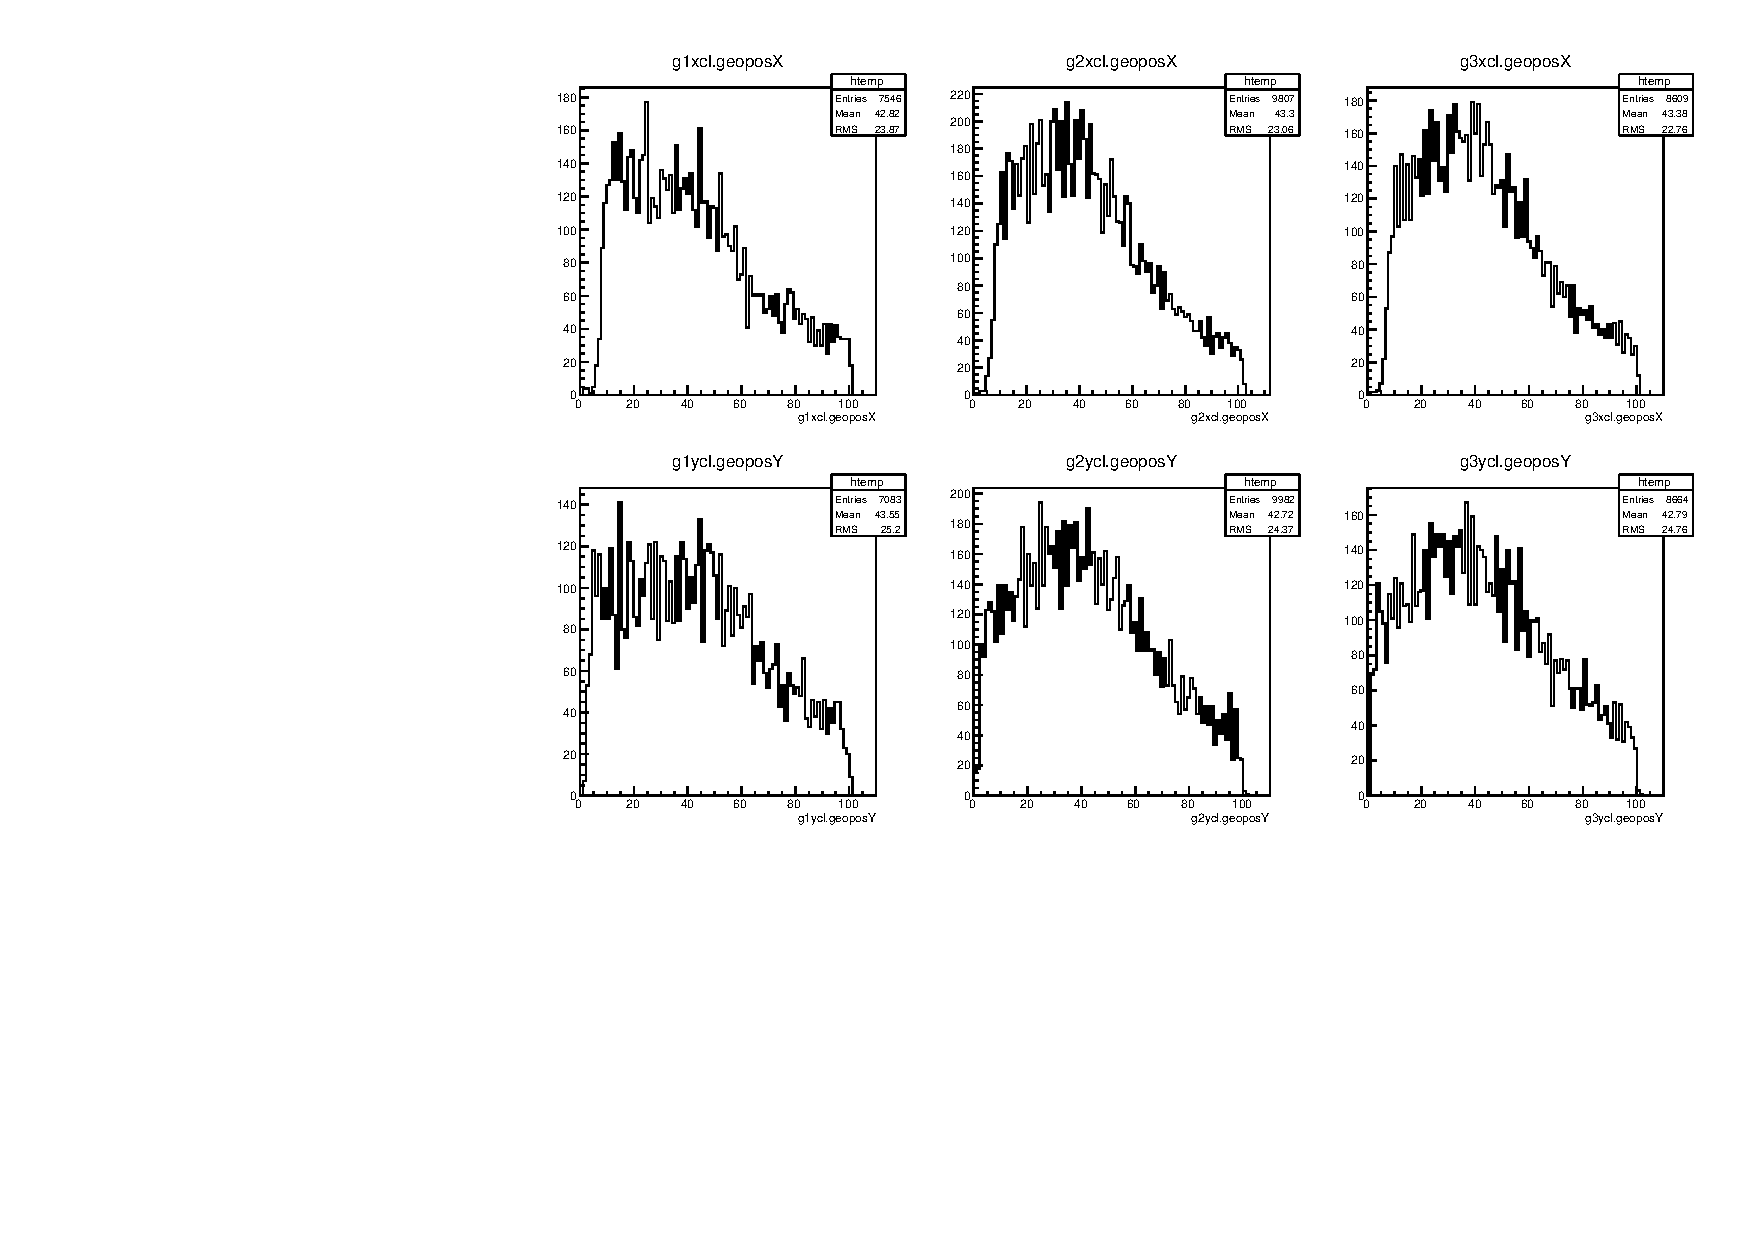
\includegraphics[width=12cm,height=8cm]{Tracker_Hit_position_1165.pdf}
%         };
%         \draw (2, 3) node {\color{red} };	% can comment anyting at a position 2,3
%         \end{tikzpicture}
\end{frame}
\begin{frame}\frametitle{Tracker Hit position 1164}
%        \begin{tikzpicture}
%         \draw (0, 0) node[inner sep=0]
 %        {
	 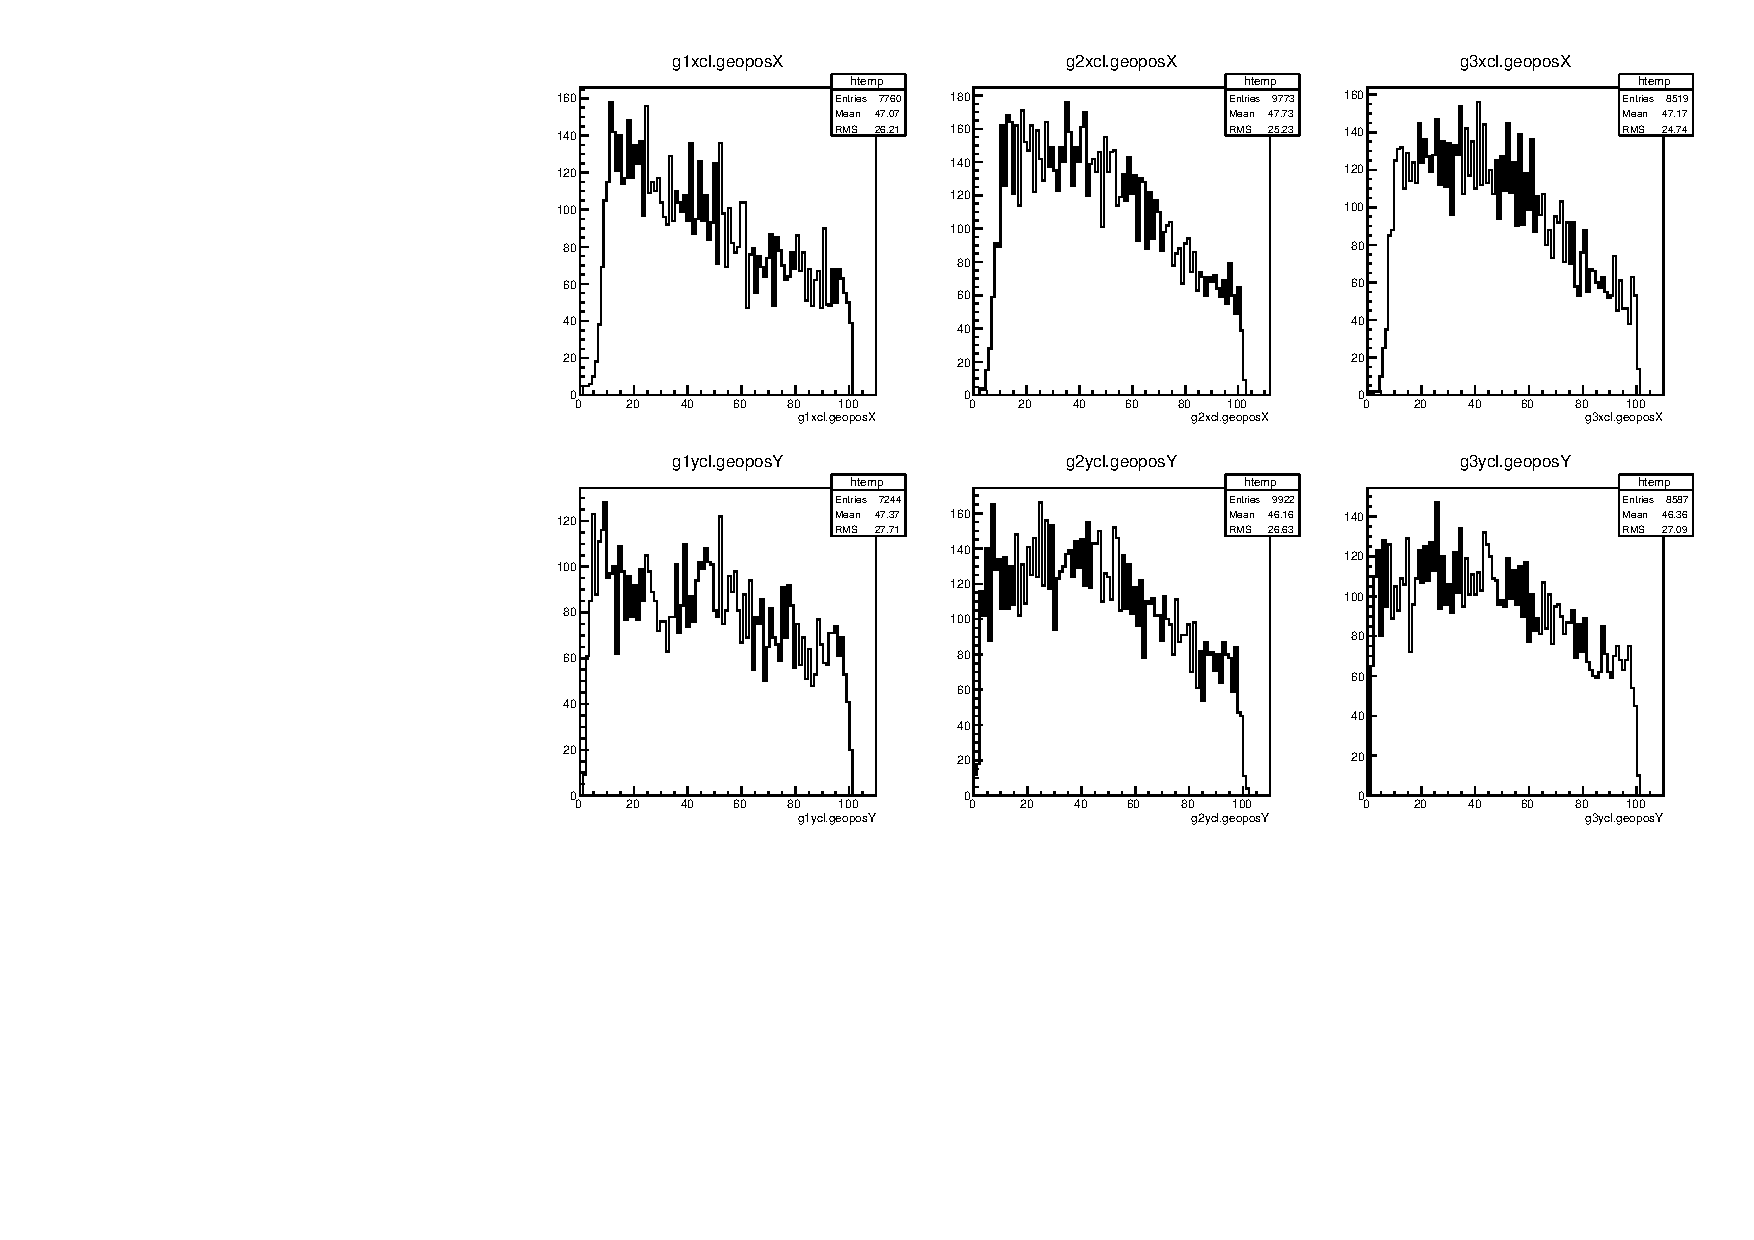
\includegraphics[width=12cm,height=8cm]{Tracker_Hit_position_1164.pdf}
%         };
%         \draw (2, 3) node {\color{red} };	% can comment anyting at a position 2,3
%         \end{tikzpicture}
\end{frame}
\begin{frame}\frametitle{Tracker Hit position 1163}
%        \begin{tikzpicture}
%         \draw (0, 0) node[inner sep=0]
 %        {
	 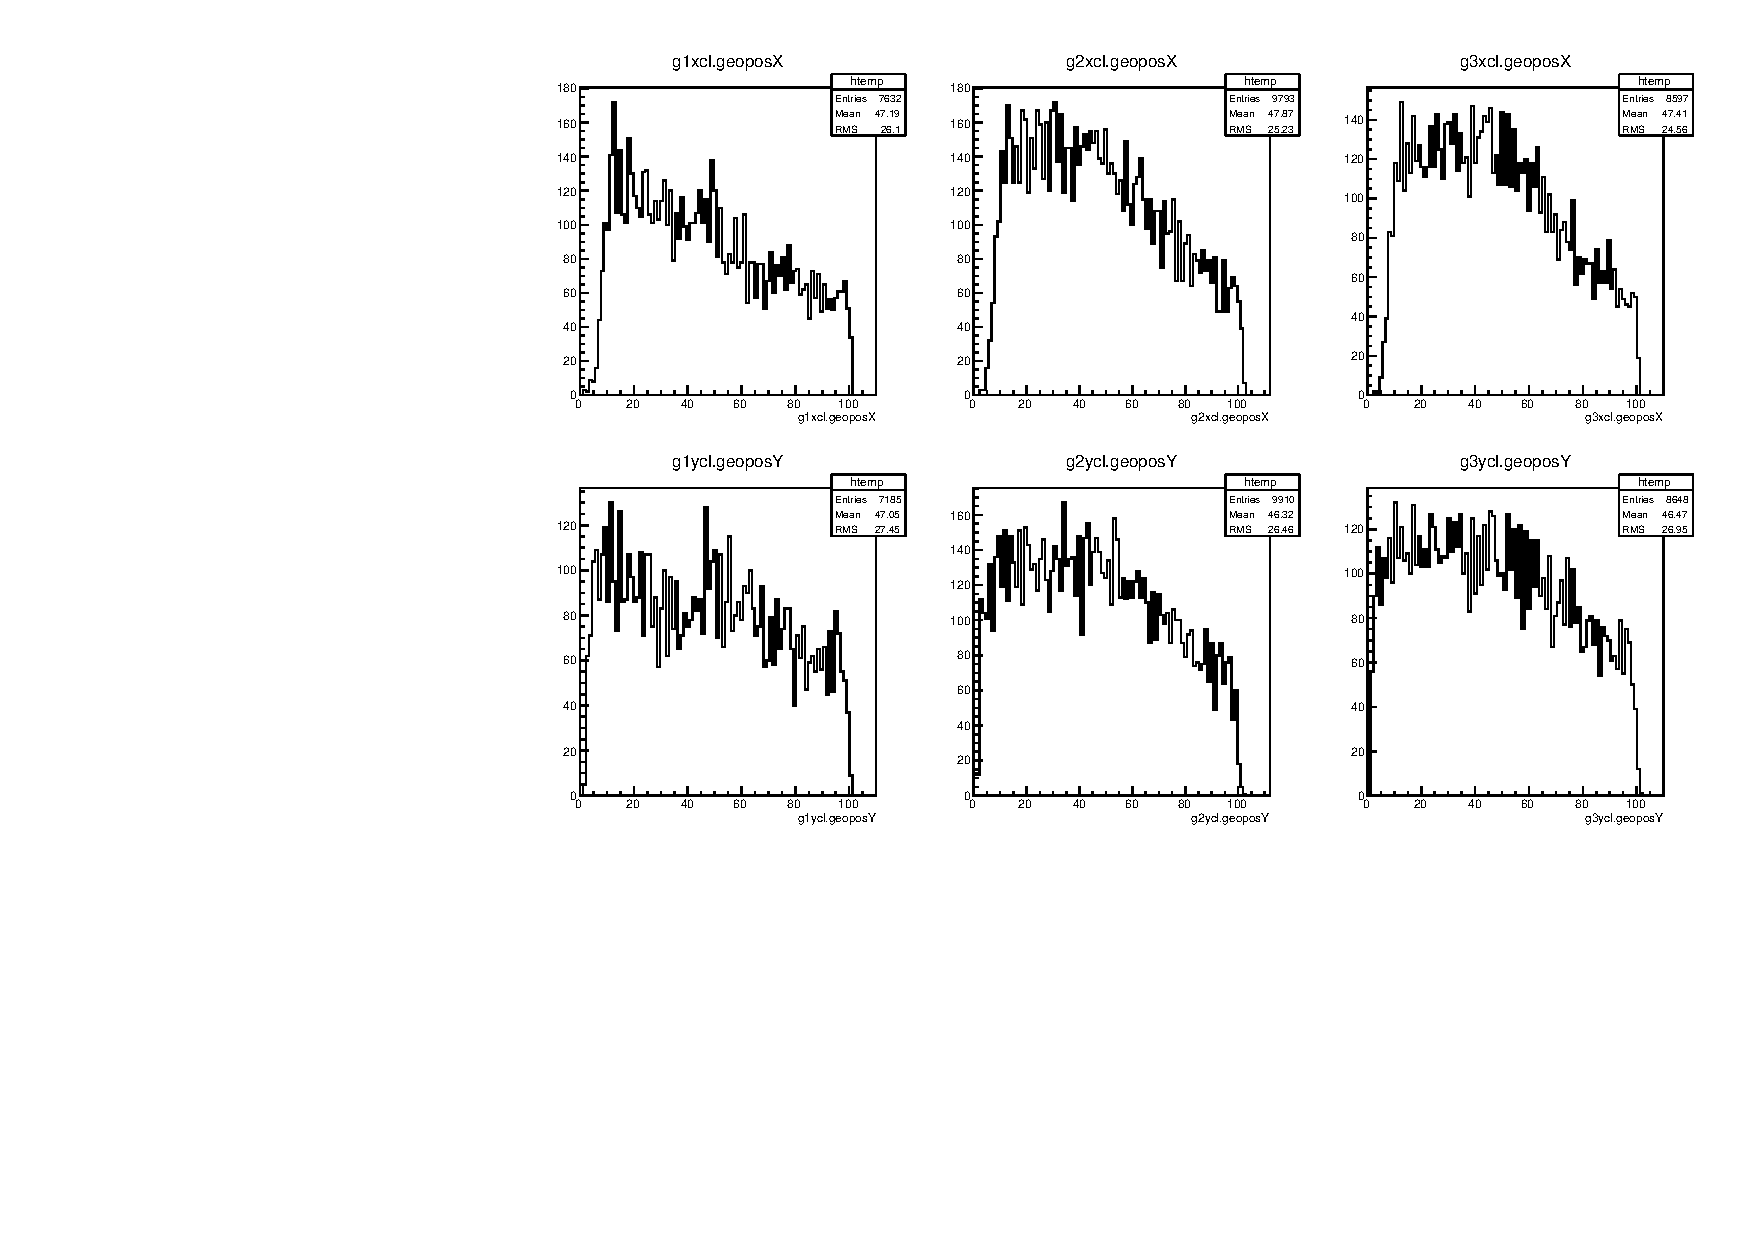
\includegraphics[width=12cm,height=8cm]{Tracker_Hit_position_1163.pdf}
%         };
%         \draw (2, 3) node {\color{red} };	% can comment anyting at a position 2,3
%         \end{tikzpicture}
\end{frame}
\begin{frame}\frametitle{Tracker Hit position 1158}
%        \begin{tikzpicture}
%         \draw (0, 0) node[inner sep=0]
 %        {
	 
\includegraphics[width=12cm,height=8cm]{Tracker_Hit_position_1158.pdf}
%         };
%         \draw (2, 3) node {\color{red} };	% can comment anyting at a position 2,3
%         \end{tikzpicture}
\end{frame}
\begin{frame}\frametitle{Tracker Hit position 1157}
%        \begin{tikzpicture}
%         \draw (0, 0) node[inner sep=0]
 %        {
	 
\includegraphics[width=12cm,height=8cm]{Tracker_Hit_position_1157.pdf}
%         };
%         \draw (2, 3) node {\color{red} };	% can comment anyting at a position 2,3
%         \end{tikzpicture}
\end{frame}
\begin{frame}\frametitle{Tracker Hit position 1156}
%        \begin{tikzpicture}
%         \draw (0, 0) node[inner sep=0]
 %        {
	 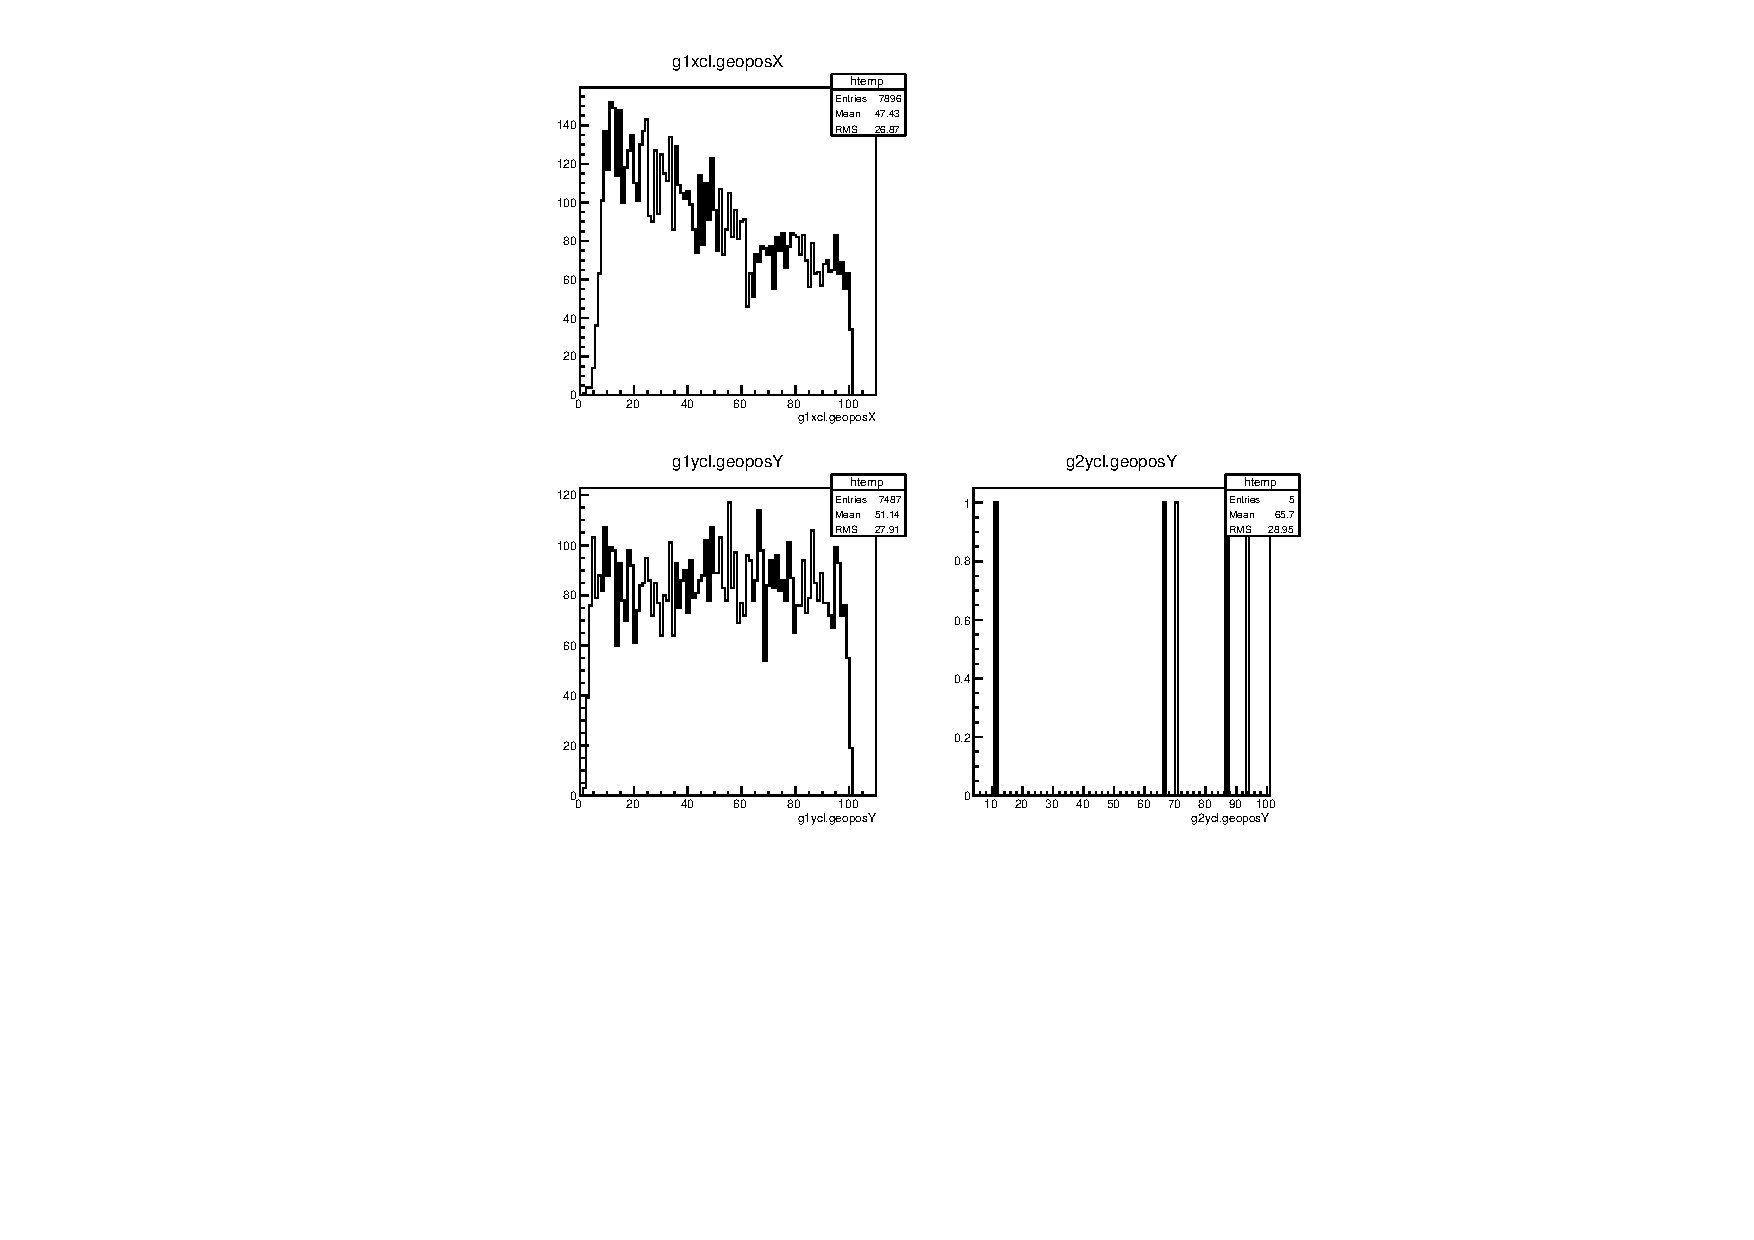
\includegraphics[width=12cm,height=8cm]{Tracker_Hit_position_1156.pdf}
%         };
%         \draw (2, 3) node {\color{red} };	% can comment anyting at a position 2,3
%         \end{tikzpicture}
\end{frame}
\begin{frame}\frametitle{Tracker Hit position 1155}
%        \begin{tikzpicture}
%         \draw (0, 0) node[inner sep=0]
 %        {
	 
\includegraphics[width=12cm,height=8cm]{Tracker_Hit_position_1155.pdf}
%         };
%         \draw (2, 3) node {\color{red} };	% can comment anyting at a position 2,3
%         \end{tikzpicture}
\end{frame}
\begin{frame}\frametitle{Tracker Hit position 1154}
%        \begin{tikzpicture}
%         \draw (0, 0) node[inner sep=0]
 %        {
	 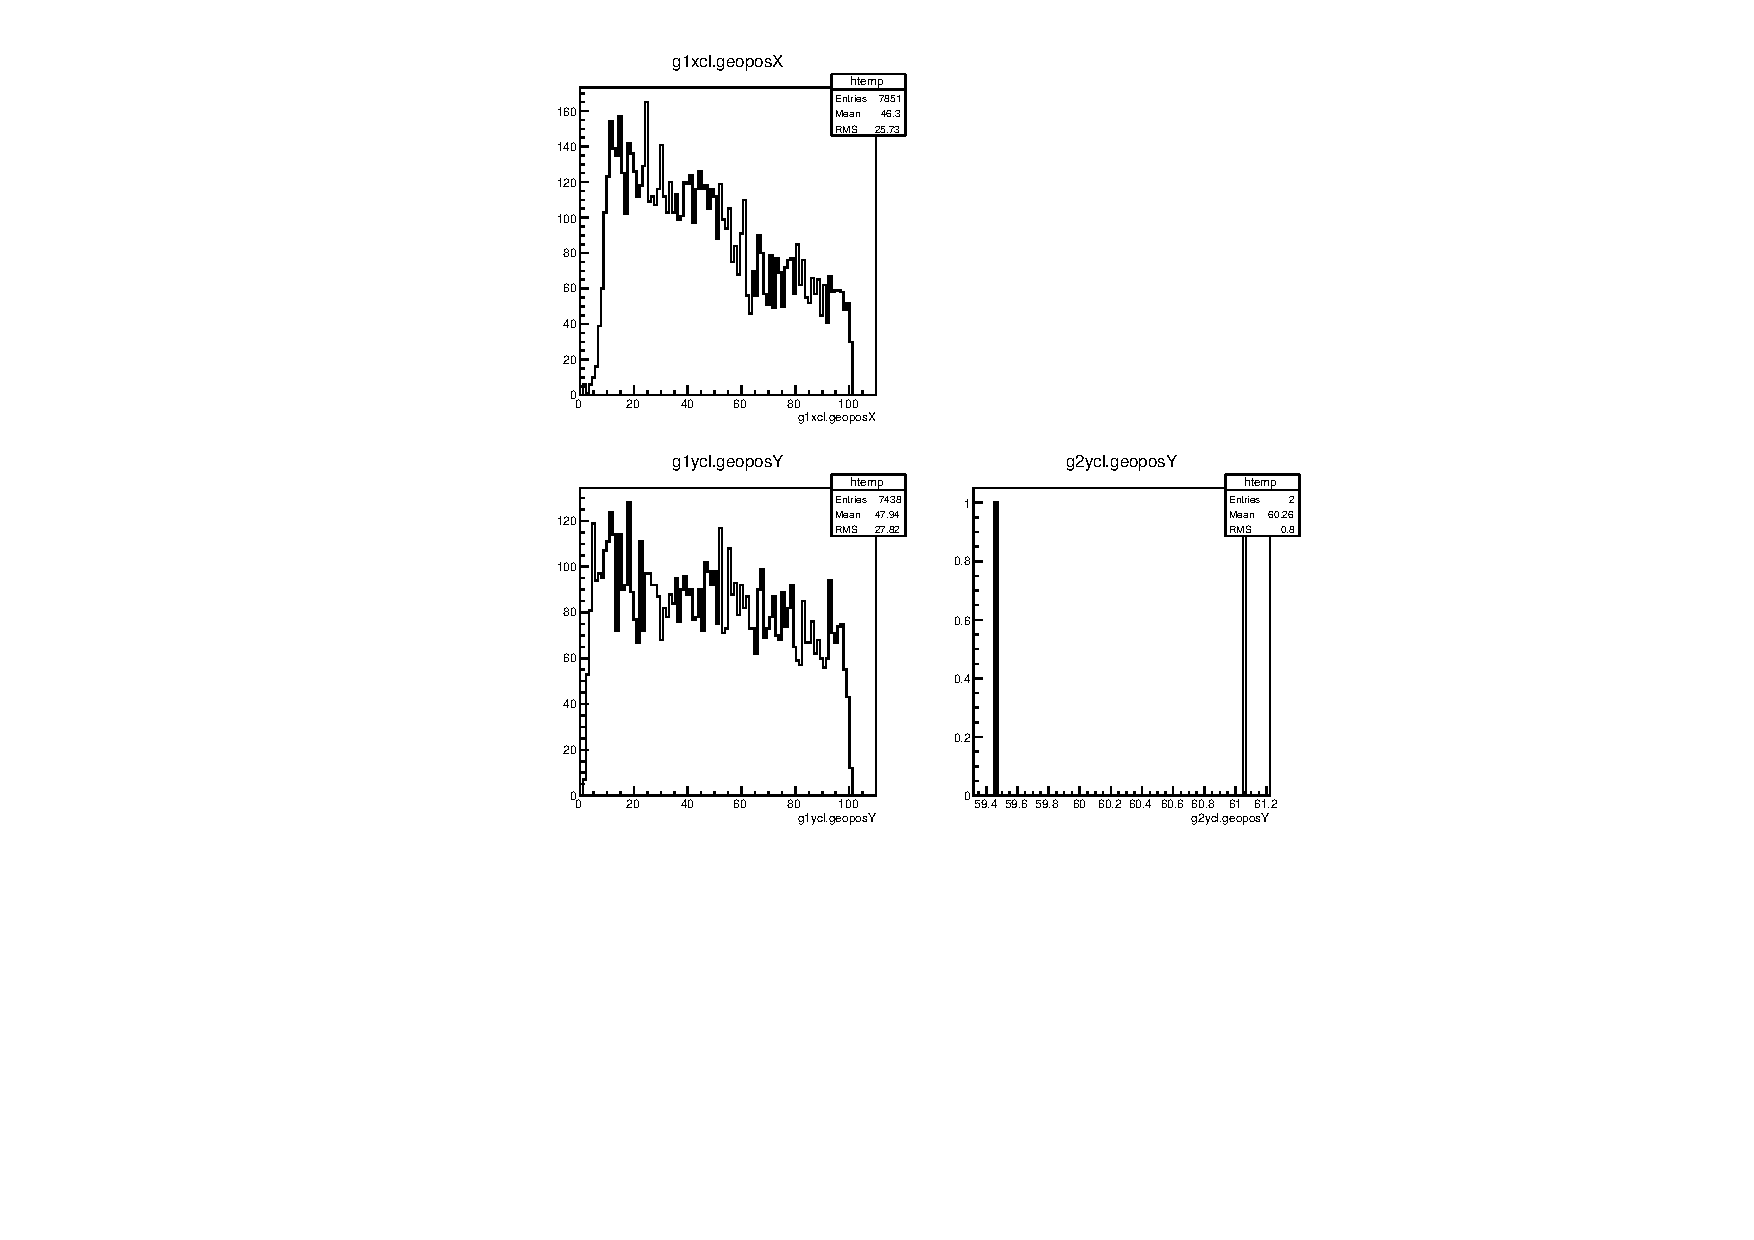
\includegraphics[width=12cm,height=8cm]{Tracker_Hit_position_1154.pdf}
%         };
%         \draw (2, 3) node {\color{red} };	% can comment anyting at a position 2,3
%         \end{tikzpicture}
\end{frame}
\begin{frame}\frametitle{Tracker Hit position 1153}
%        \begin{tikzpicture}
%         \draw (0, 0) node[inner sep=0]
 %        {
	 
\includegraphics[width=12cm,height=8cm]{Tracker_Hit_position_1153.pdf}
%         };
%         \draw (2, 3) node {\color{red} };	% can comment anyting at a position 2,3
%         \end{tikzpicture}
\end{frame}
\begin{frame}\frametitle{Tracker Hit position 1152}
%        \begin{tikzpicture}
%         \draw (0, 0) node[inner sep=0]
 %        {
	 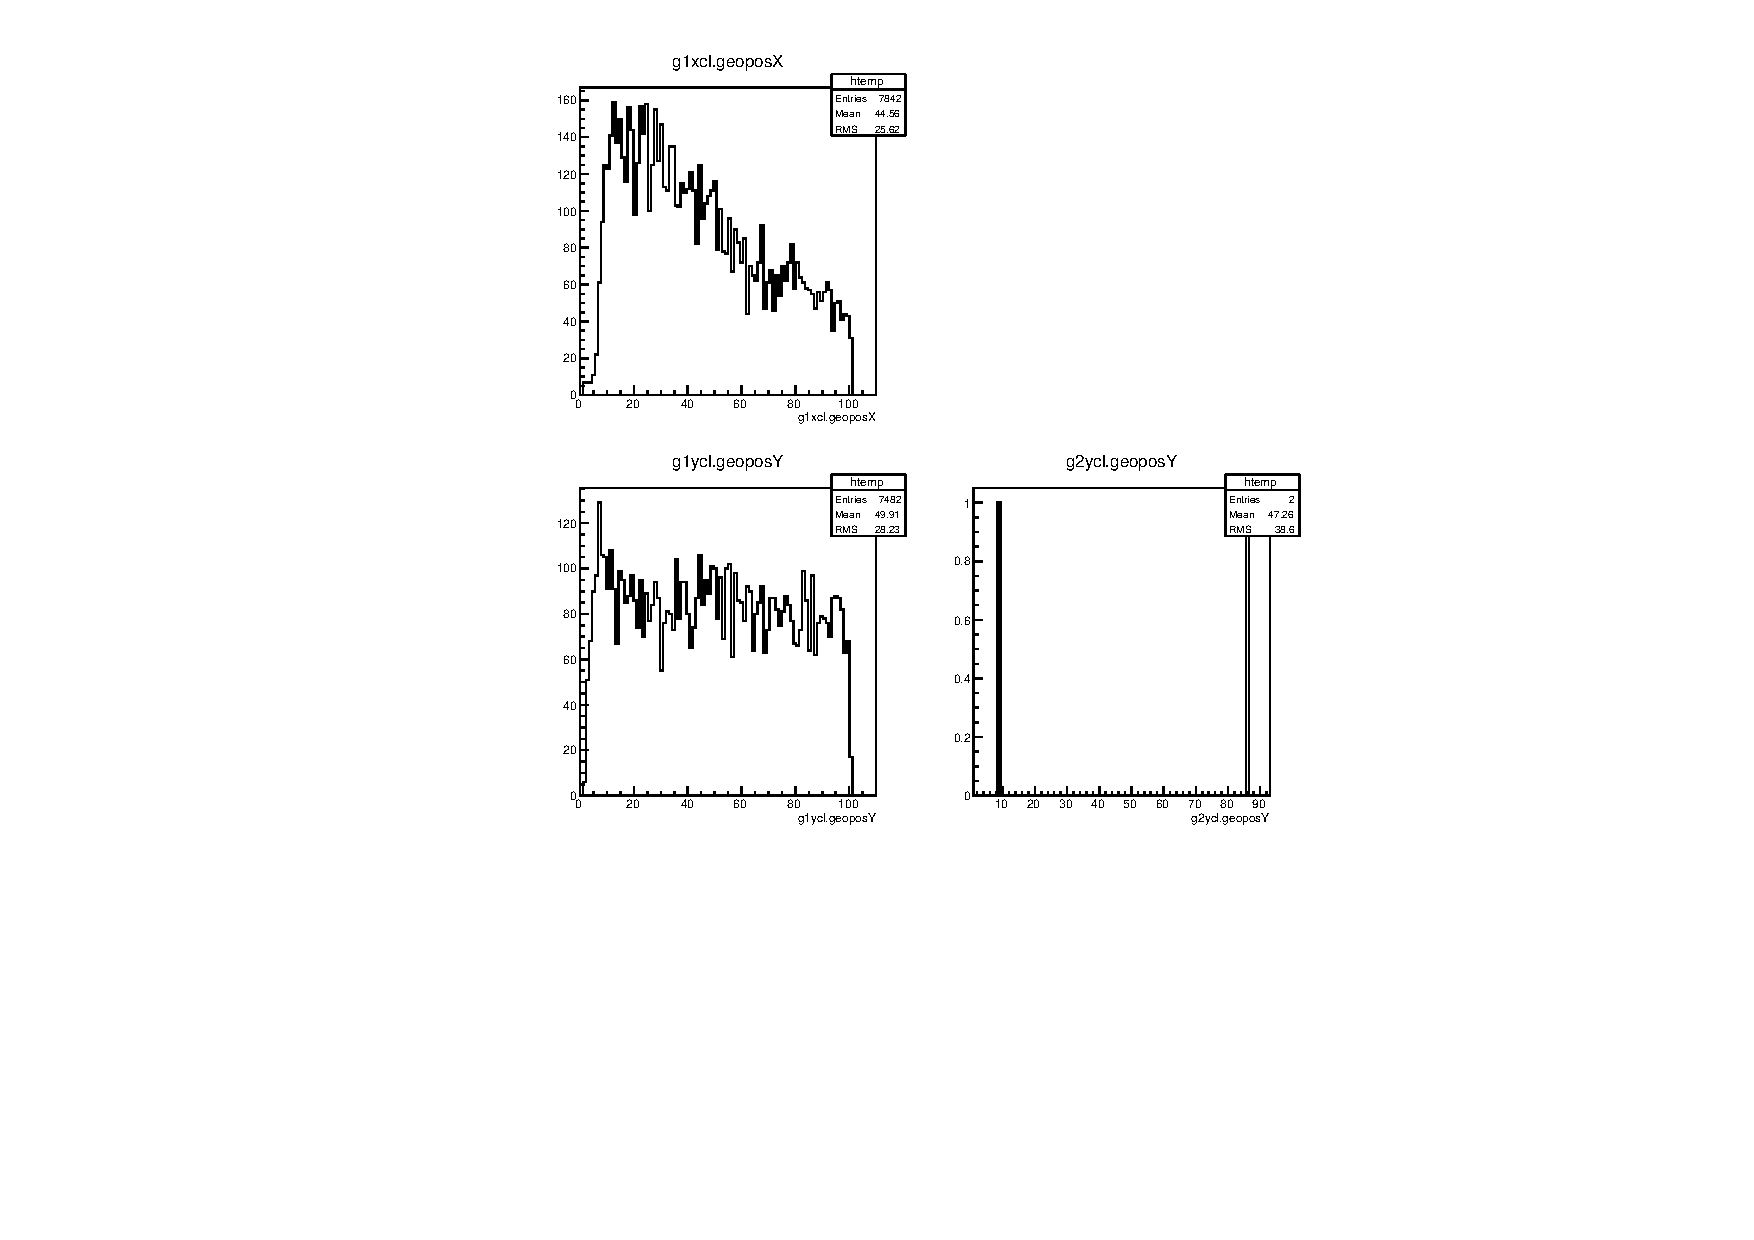
\includegraphics[width=12cm,height=8cm]{Tracker_Hit_position_1152.pdf}
%         };
%         \draw (2, 3) node {\color{red} };	% can comment anyting at a position 2,3
%         \end{tikzpicture}
\end{frame}
\begin{frame}\frametitle{Tracker Hit position 1151}
%        \begin{tikzpicture}
%         \draw (0, 0) node[inner sep=0]
 %        {
	 
\includegraphics[width=12cm,height=8cm]{Tracker_Hit_position_1151.pdf}
%         };
%         \draw (2, 3) node {\color{red} };	% can comment anyting at a position 2,3
%         \end{tikzpicture}
\end{frame}
\begin{frame}\frametitle{Tracker Hit position 1150}
%        \begin{tikzpicture}
%         \draw (0, 0) node[inner sep=0]
 %        {
	 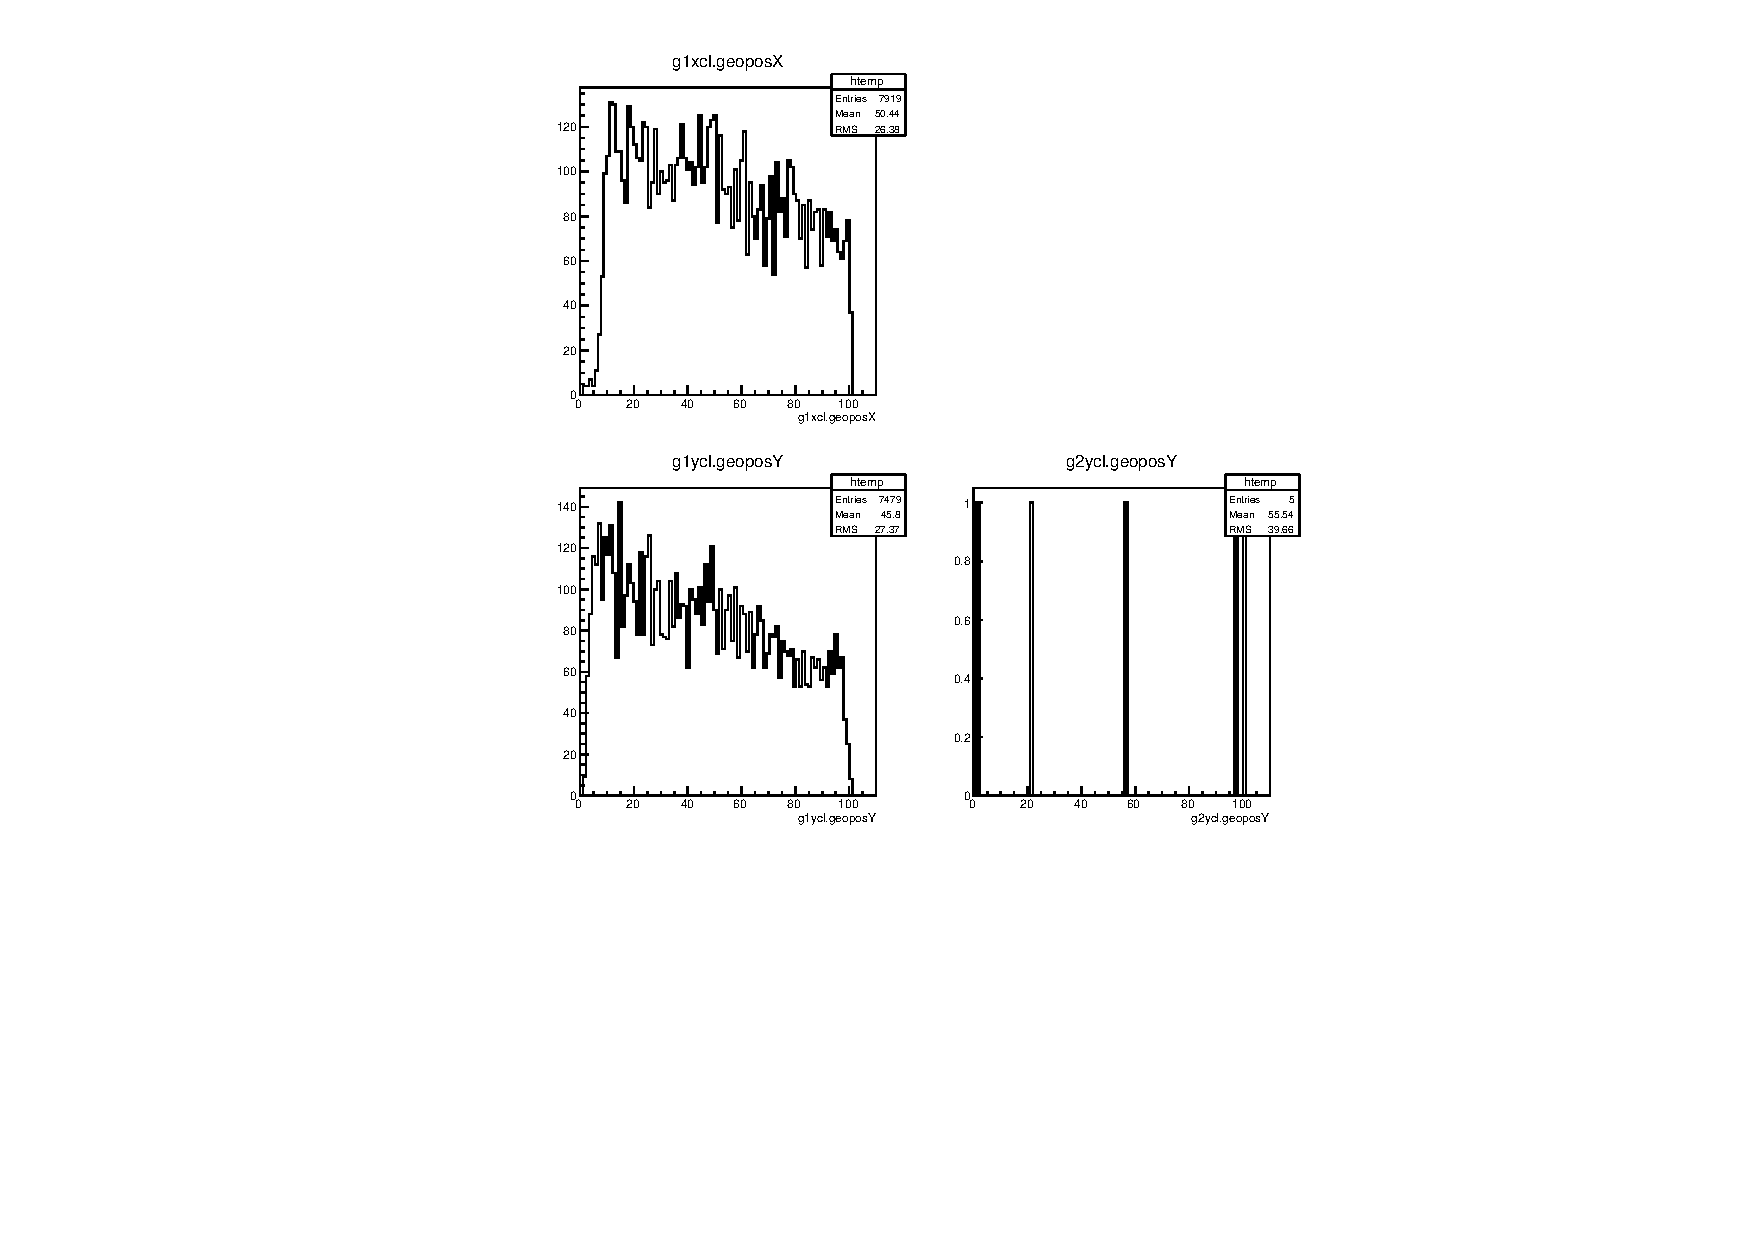
\includegraphics[width=12cm,height=8cm]{Tracker_Hit_position_1150.pdf}
%         };
%         \draw (2, 3) node {\color{red} };	% can comment anyting at a position 2,3
%         \end{tikzpicture}
\end{frame}
\begin{frame}\frametitle{Tracker Hit position 1149}
%        \begin{tikzpicture}
%         \draw (0, 0) node[inner sep=0]
 %        {
	 
\includegraphics[width=12cm,height=8cm]{Tracker_Hit_position_1149.pdf}
%         };
%         \draw (2, 3) node {\color{red} };	% can comment anyting at a position 2,3
%         \end{tikzpicture}
\end{frame}
\begin{frame}\frametitle{Tracker Hit position 1147}
%        \begin{tikzpicture}
%         \draw (0, 0) node[inner sep=0]
 %        {
	 
\includegraphics[width=12cm,height=8cm]{Tracker_Hit_position_1147.pdf}
%         };
%         \draw (2, 3) node {\color{red} };	% can comment anyting at a position 2,3
%         \end{tikzpicture}
\end{frame}
\begin{frame}\frametitle{Tracker Hit position 1146}
%        \begin{tikzpicture}
%         \draw (0, 0) node[inner sep=0]
 %        {
	 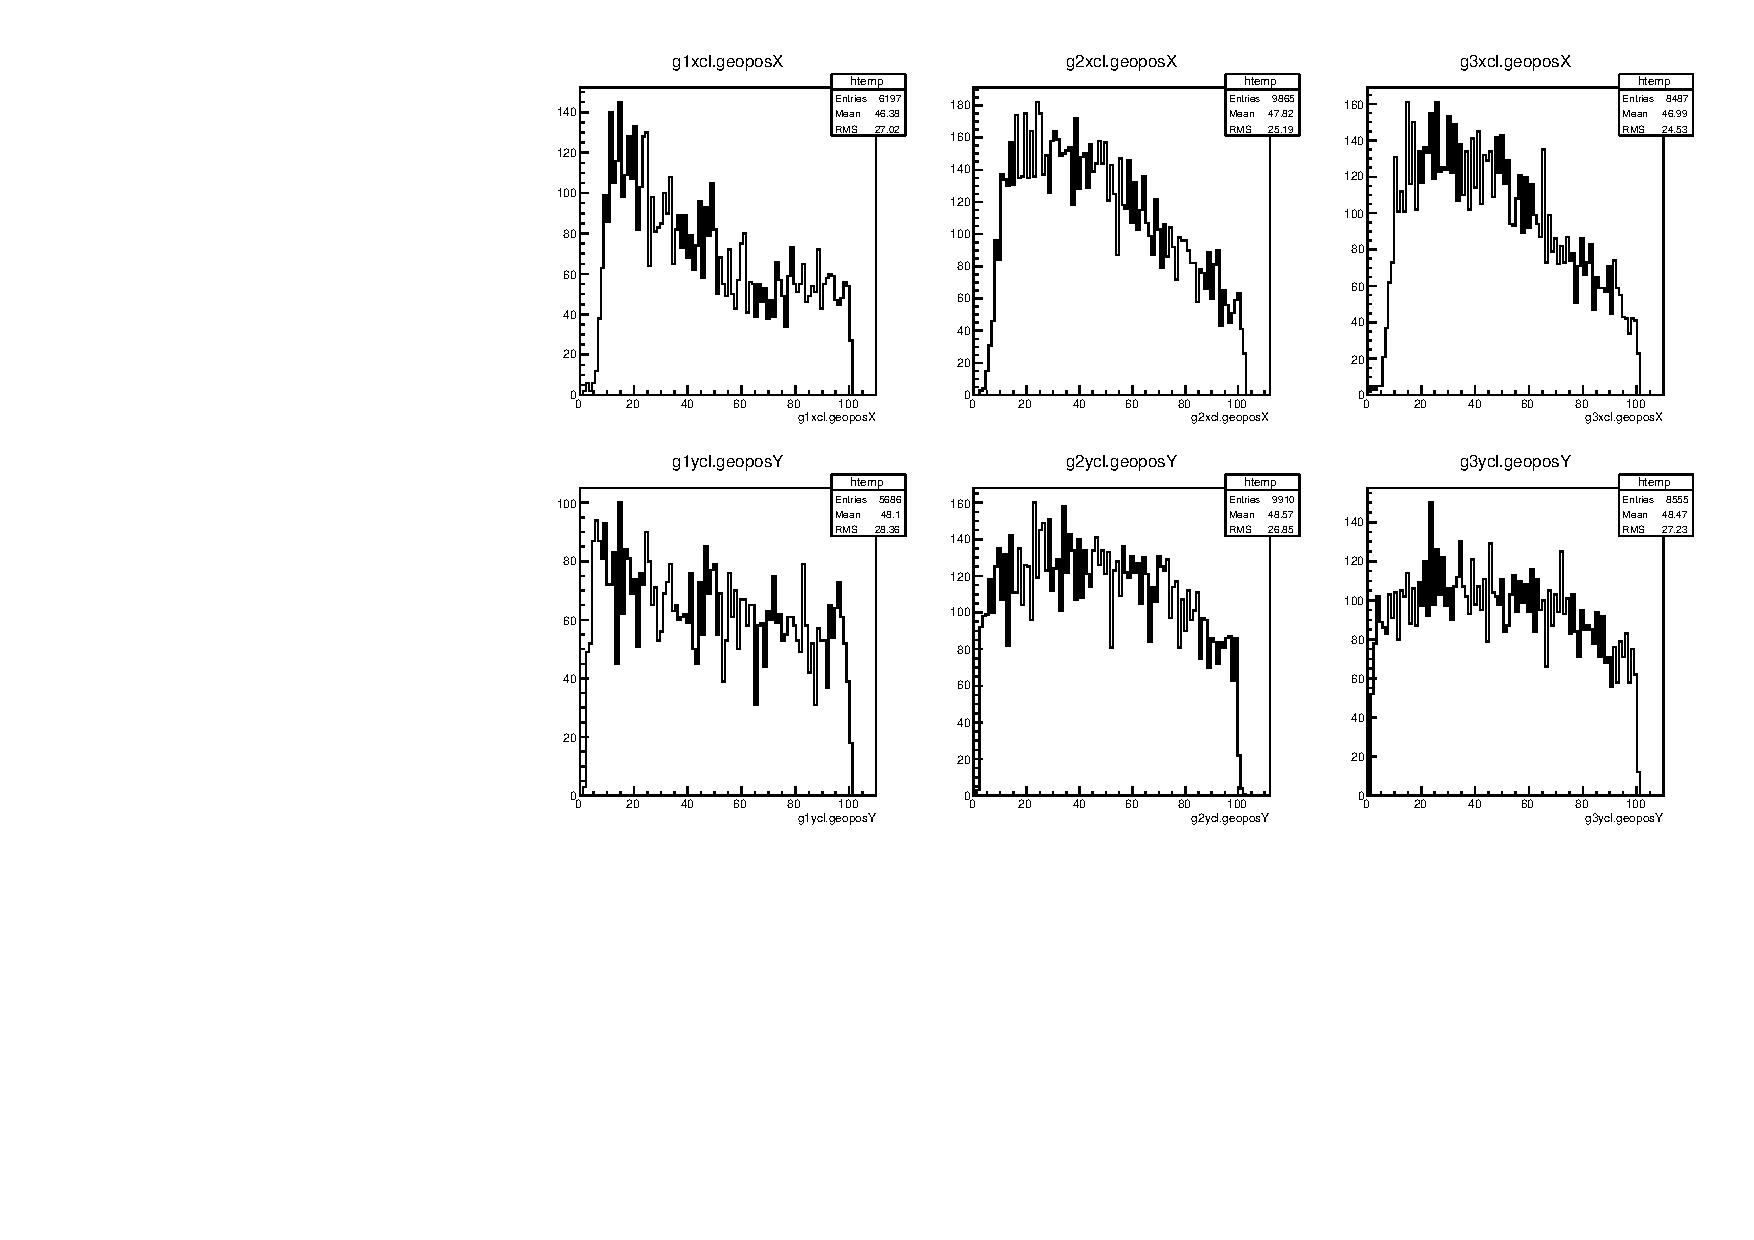
\includegraphics[width=12cm,height=8cm]{Tracker_Hit_position_1146.pdf}
%         };
%         \draw (2, 3) node {\color{red} };	% can comment anyting at a position 2,3
%         \end{tikzpicture}
\end{frame}
\begin{frame}\frametitle{Tracker Hit position 1145}
%        \begin{tikzpicture}
%         \draw (0, 0) node[inner sep=0]
 %        {
	 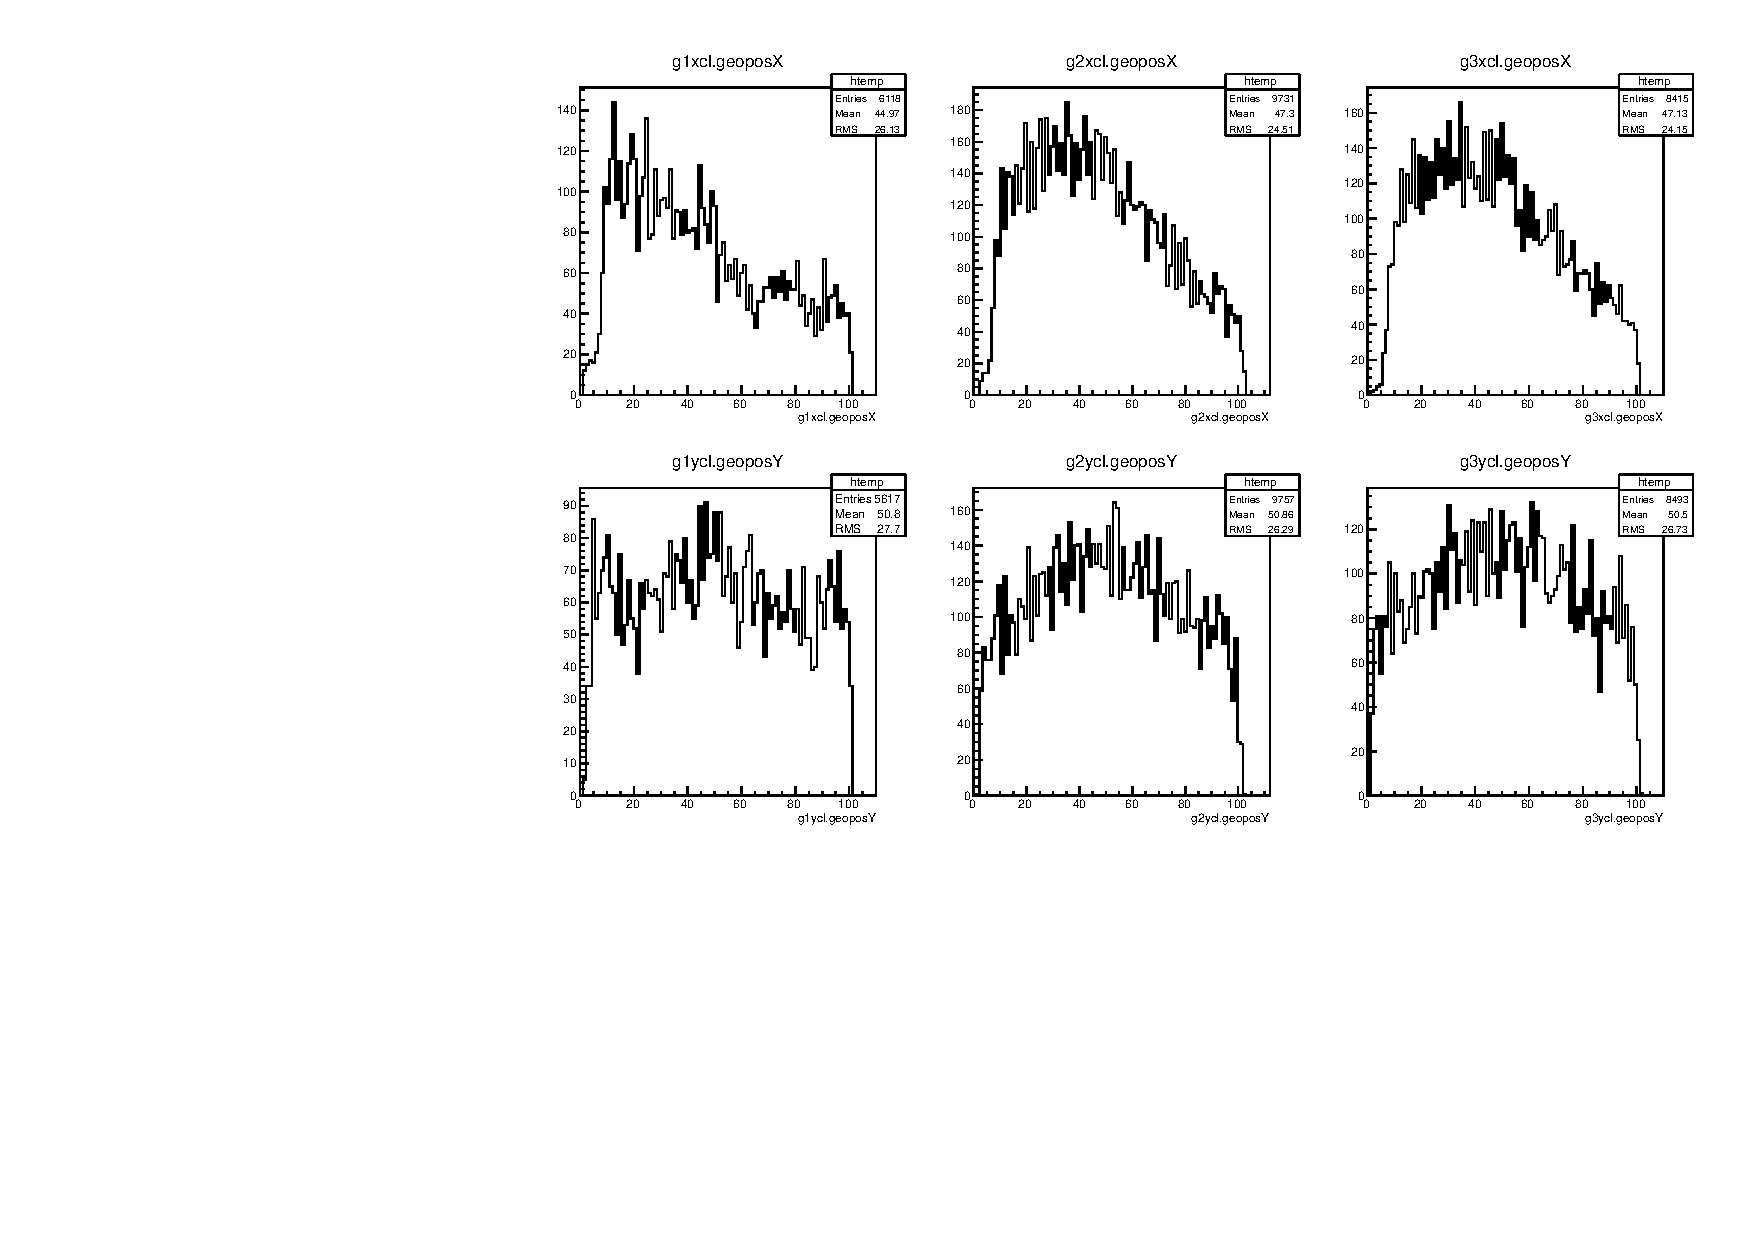
\includegraphics[width=12cm,height=8cm]{Tracker_Hit_position_1145.pdf}
%         };
%         \draw (2, 3) node {\color{red} };	% can comment anyting at a position 2,3
%         \end{tikzpicture}
\end{frame}
\begin{frame}\frametitle{Tracker Hit position 1141}
%        \begin{tikzpicture}
%         \draw (0, 0) node[inner sep=0]
 %        {
	 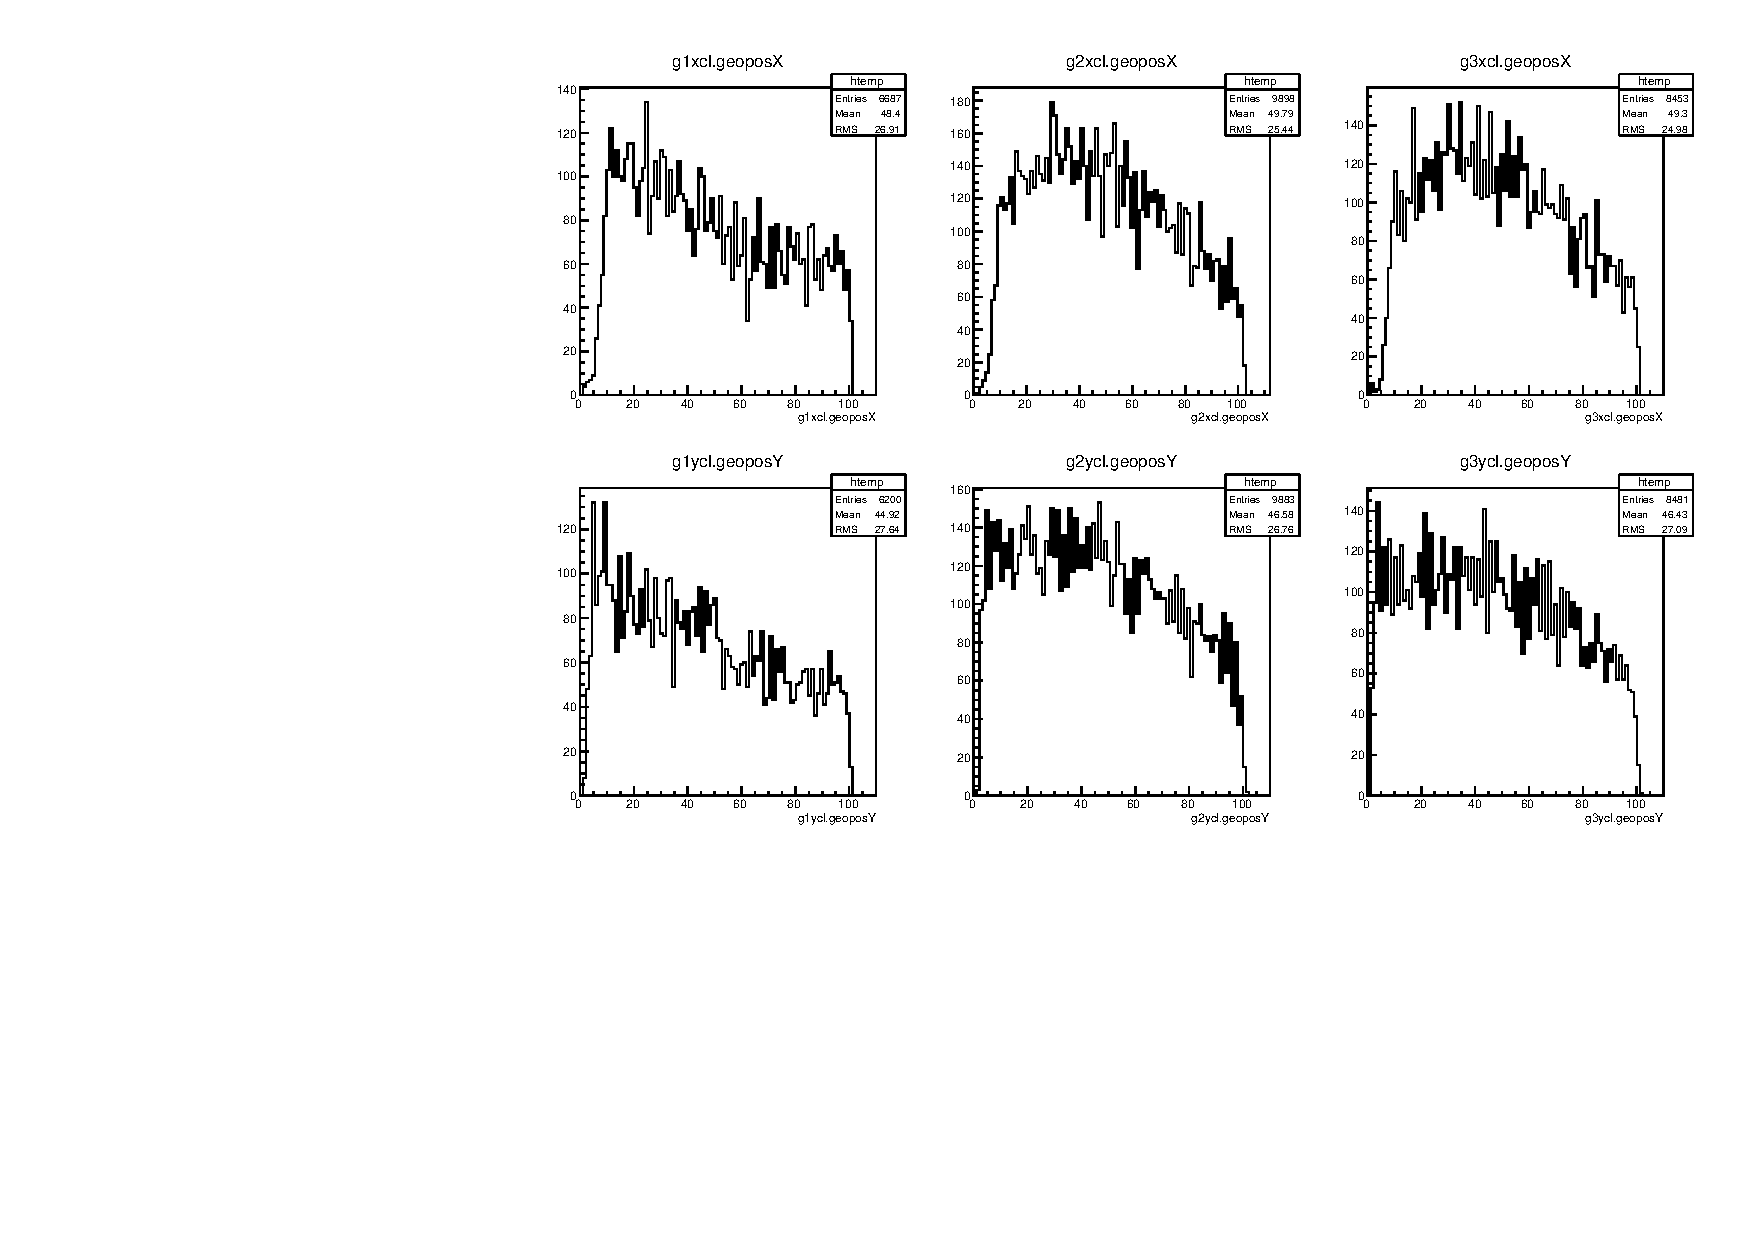
\includegraphics[width=12cm,height=8cm]{Tracker_Hit_position_1141.pdf}
%         };
%         \draw (2, 3) node {\color{red} };	% can comment anyting at a position 2,3
%         \end{tikzpicture}
\end{frame}
\begin{frame}\frametitle{Tracker Hit position 1140}
%        \begin{tikzpicture}
%         \draw (0, 0) node[inner sep=0]
 %        {
	 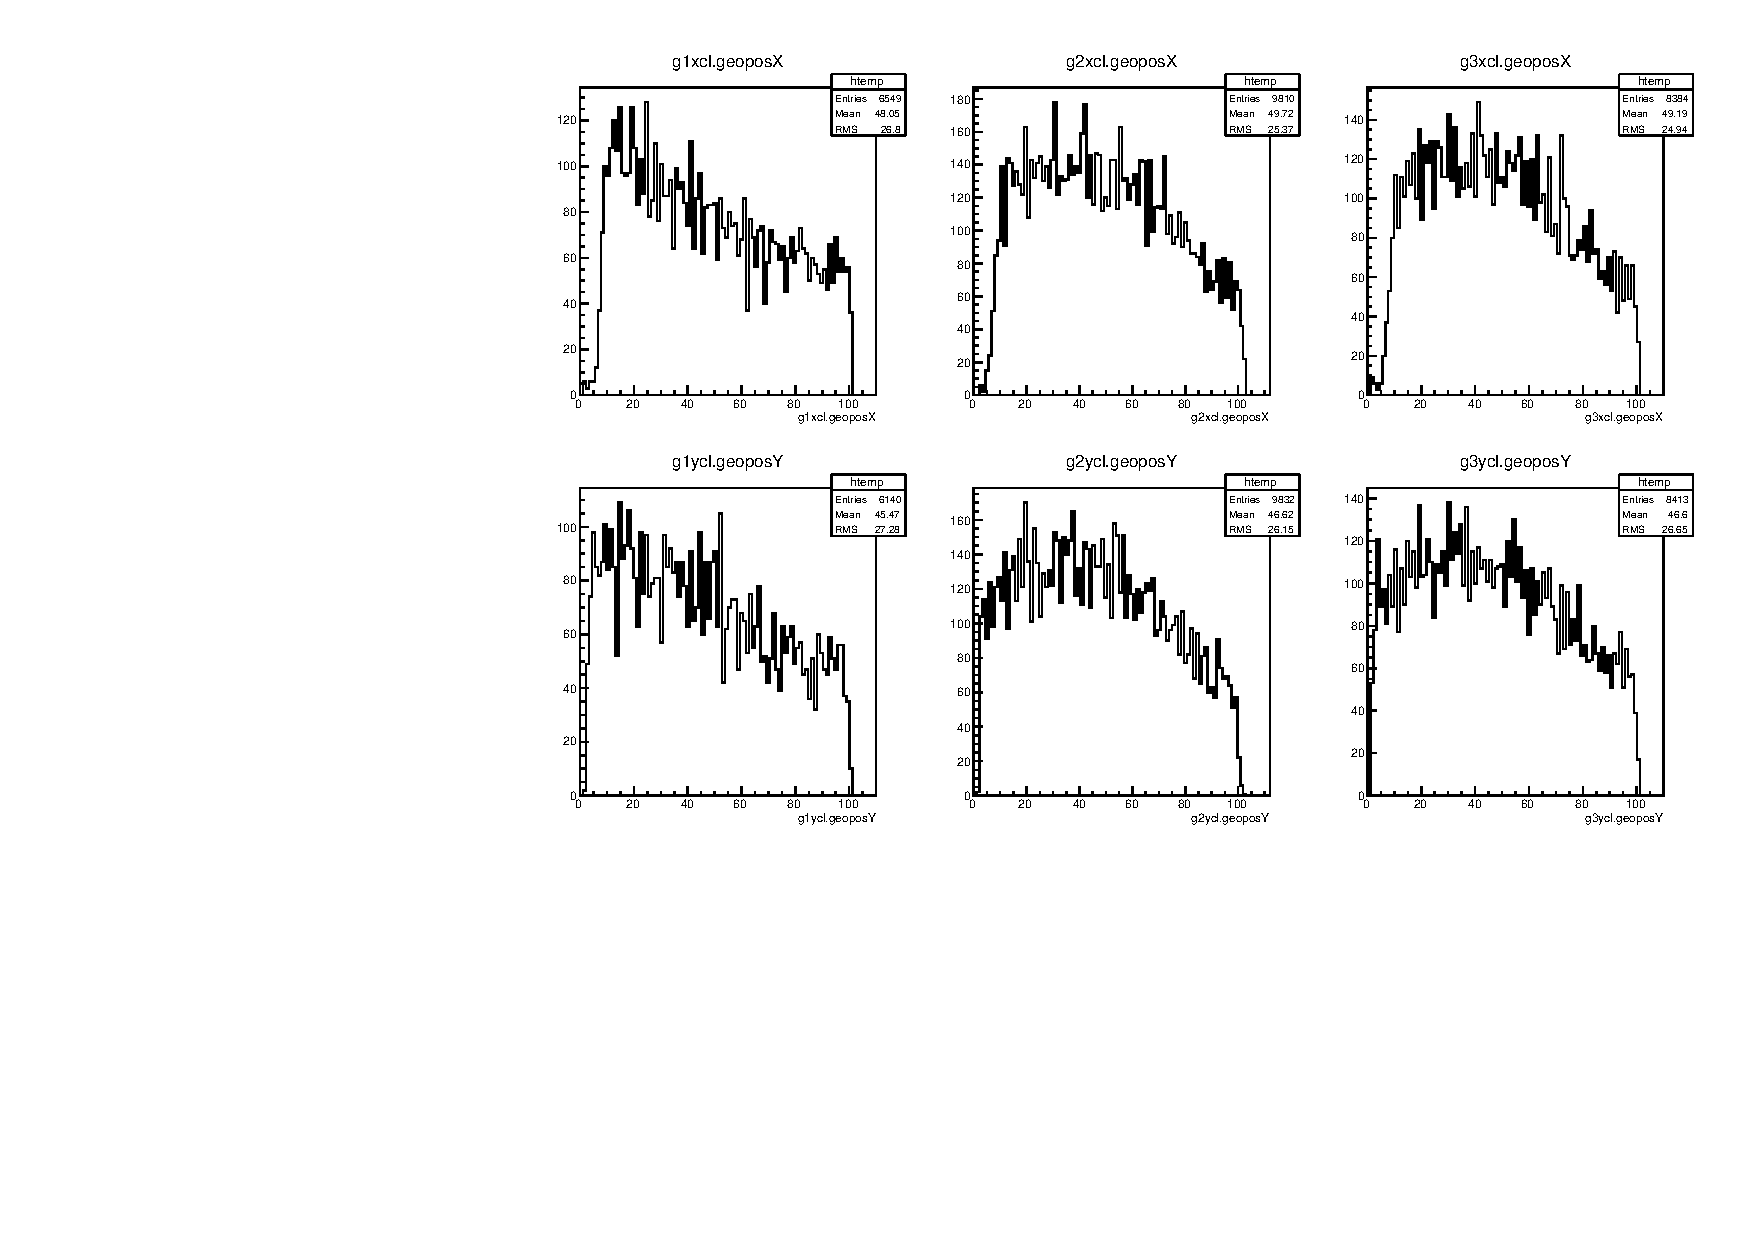
\includegraphics[width=12cm,height=8cm]{Tracker_Hit_position_1140.pdf}
%         };
%         \draw (2, 3) node {\color{red} };	% can comment anyting at a position 2,3
%         \end{tikzpicture}
\end{frame}
\begin{frame}\frametitle{Tracker Hit position 1139}
%        \begin{tikzpicture}
%         \draw (0, 0) node[inner sep=0]
 %        {
	 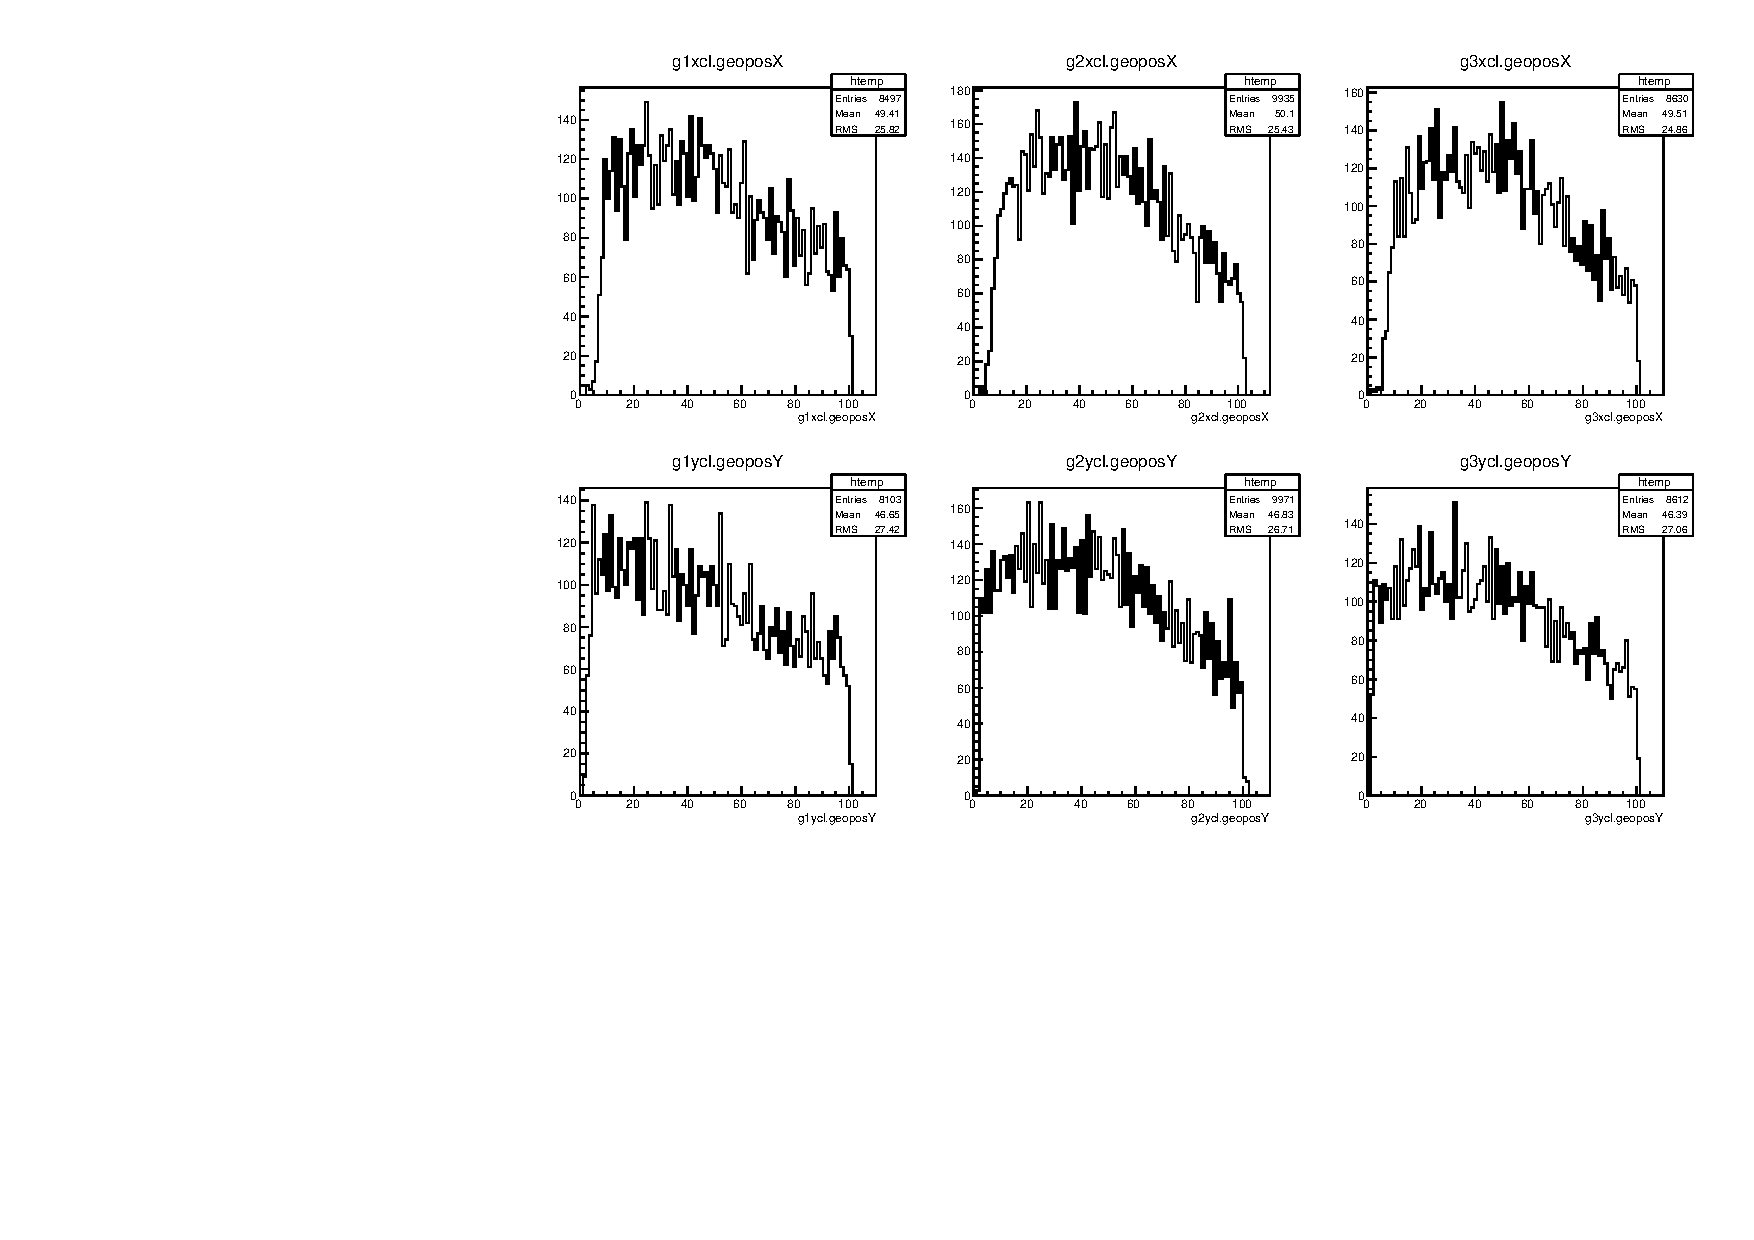
\includegraphics[width=12cm,height=8cm]{Tracker_Hit_position_1139.pdf}
%         };
%         \draw (2, 3) node {\color{red} };	% can comment anyting at a position 2,3
%         \end{tikzpicture}
\end{frame}
\begin{frame}\frametitle{Tracker Hit position 1138}
%        \begin{tikzpicture}
%         \draw (0, 0) node[inner sep=0]
 %        {
	 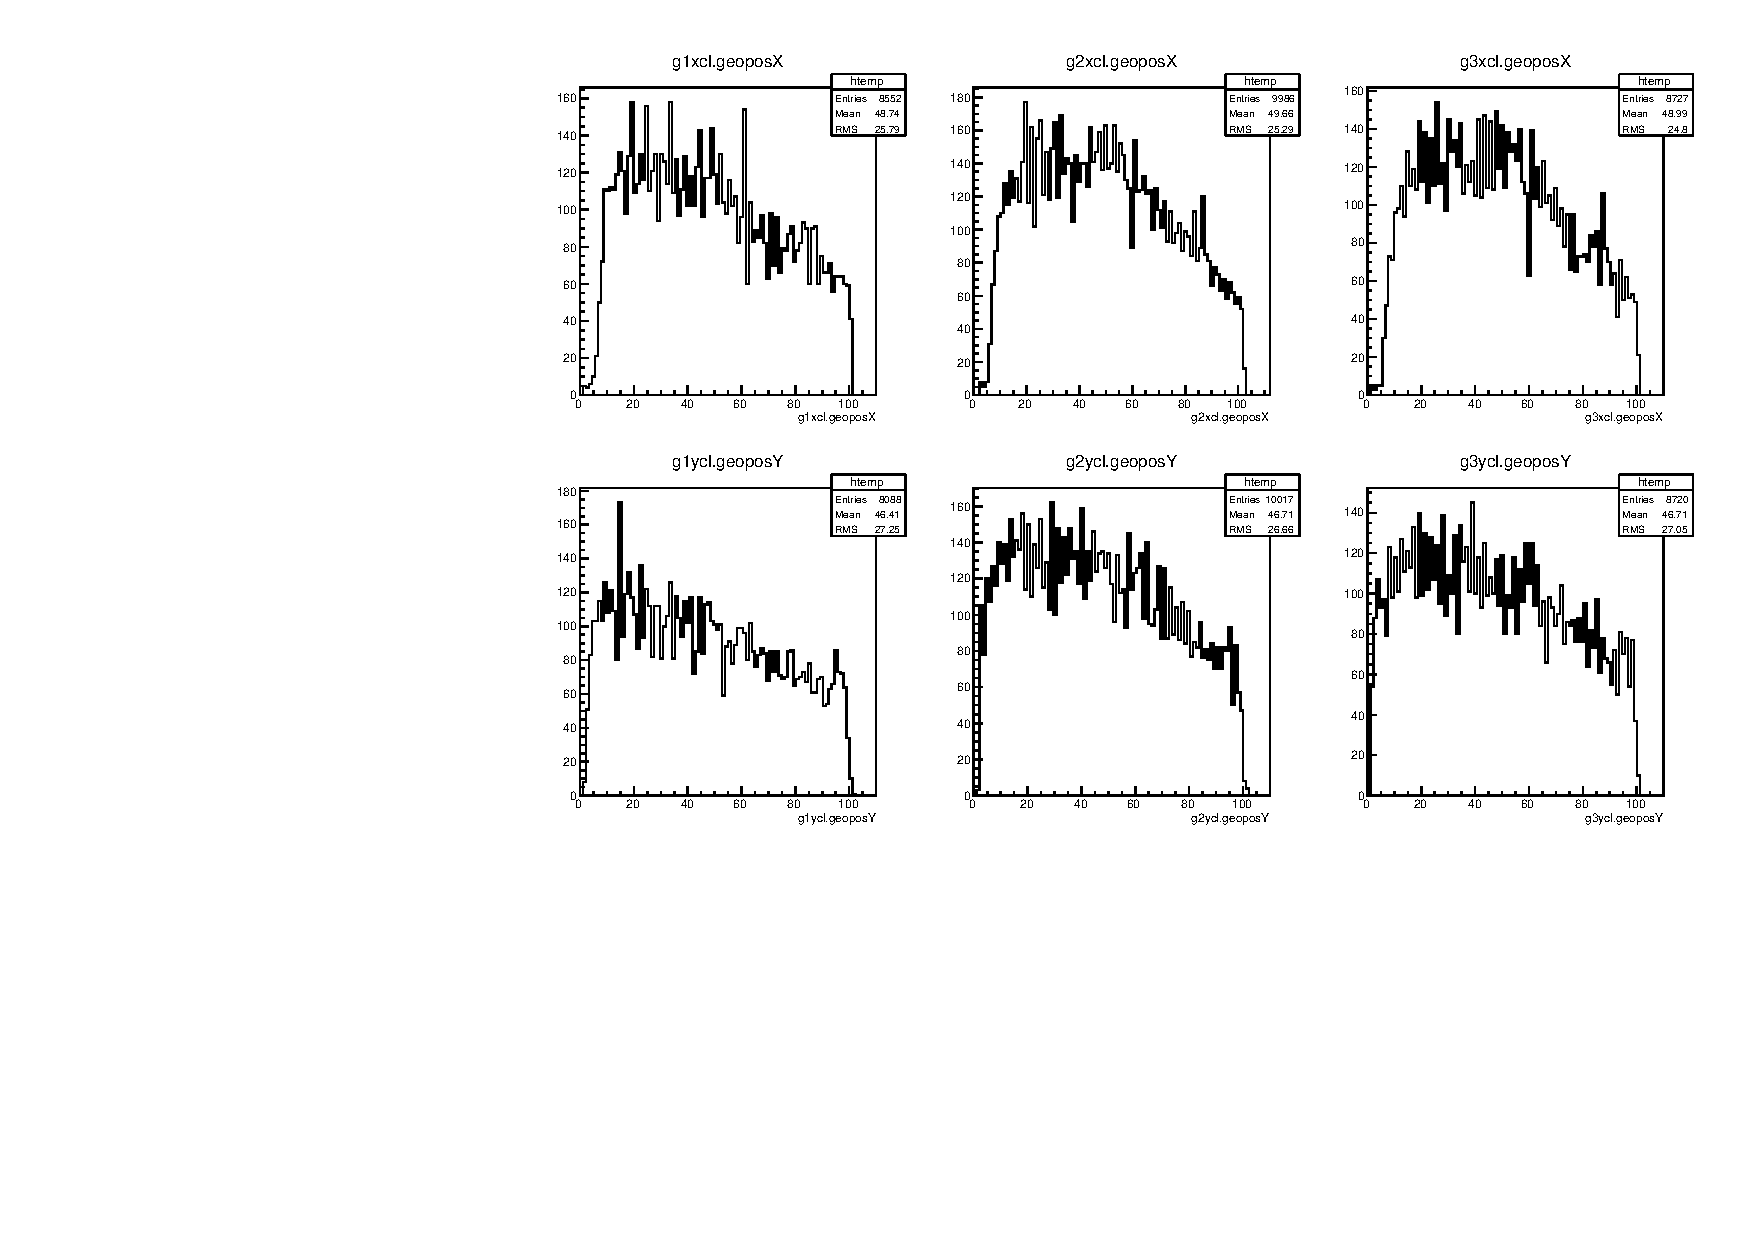
\includegraphics[width=12cm,height=8cm]{Tracker_Hit_position_1138.pdf}
%         };
%         \draw (2, 3) node {\color{red} };	% can comment anyting at a position 2,3
%         \end{tikzpicture}
\end{frame}
\begin{frame}\frametitle{Tracker Hit position 1137}
%        \begin{tikzpicture}
%         \draw (0, 0) node[inner sep=0]
 %        {
	 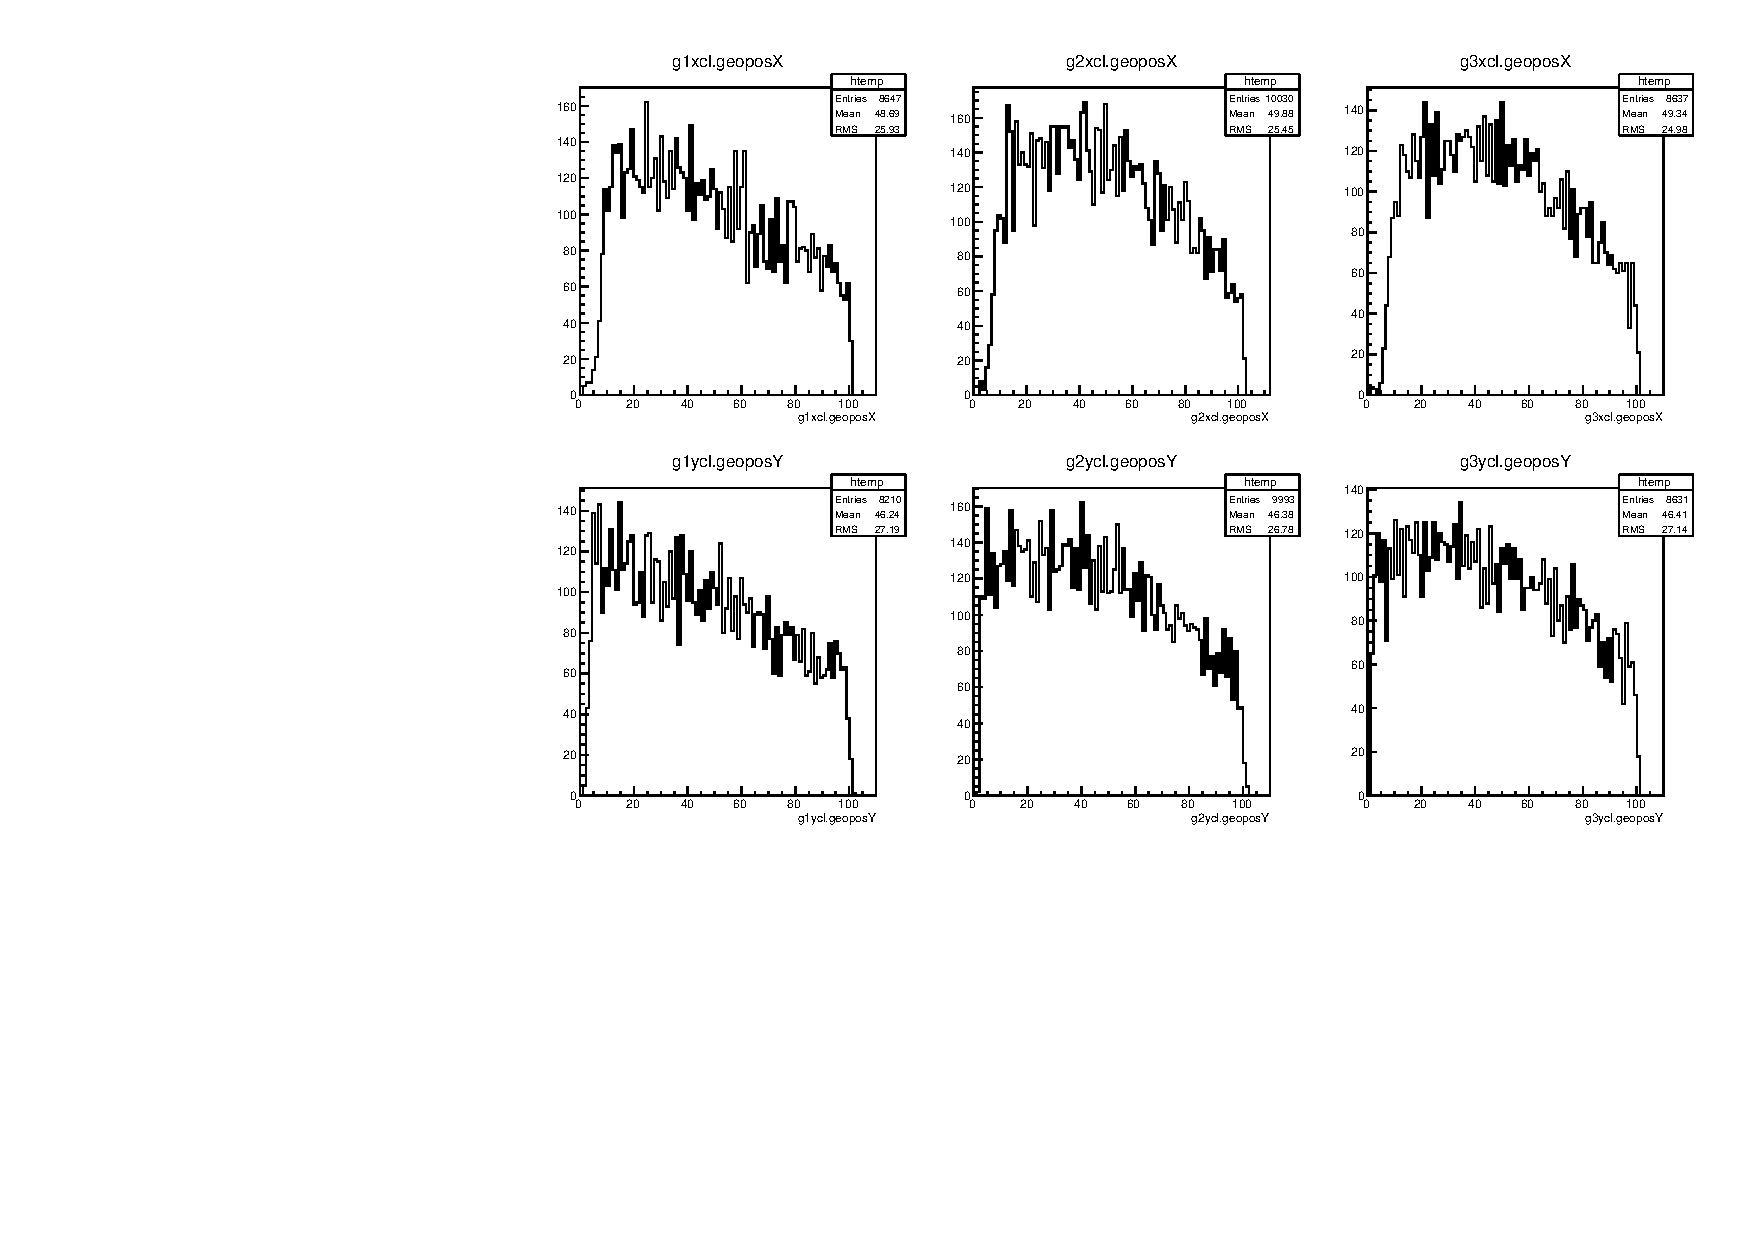
\includegraphics[width=12cm,height=8cm]{Tracker_Hit_position_1137.pdf}
%         };
%         \draw (2, 3) node {\color{red} };	% can comment anyting at a position 2,3
%         \end{tikzpicture}
\end{frame}
\begin{frame}\frametitle{Tracker Hit position 1136}
%        \begin{tikzpicture}
%         \draw (0, 0) node[inner sep=0]
 %        {
	 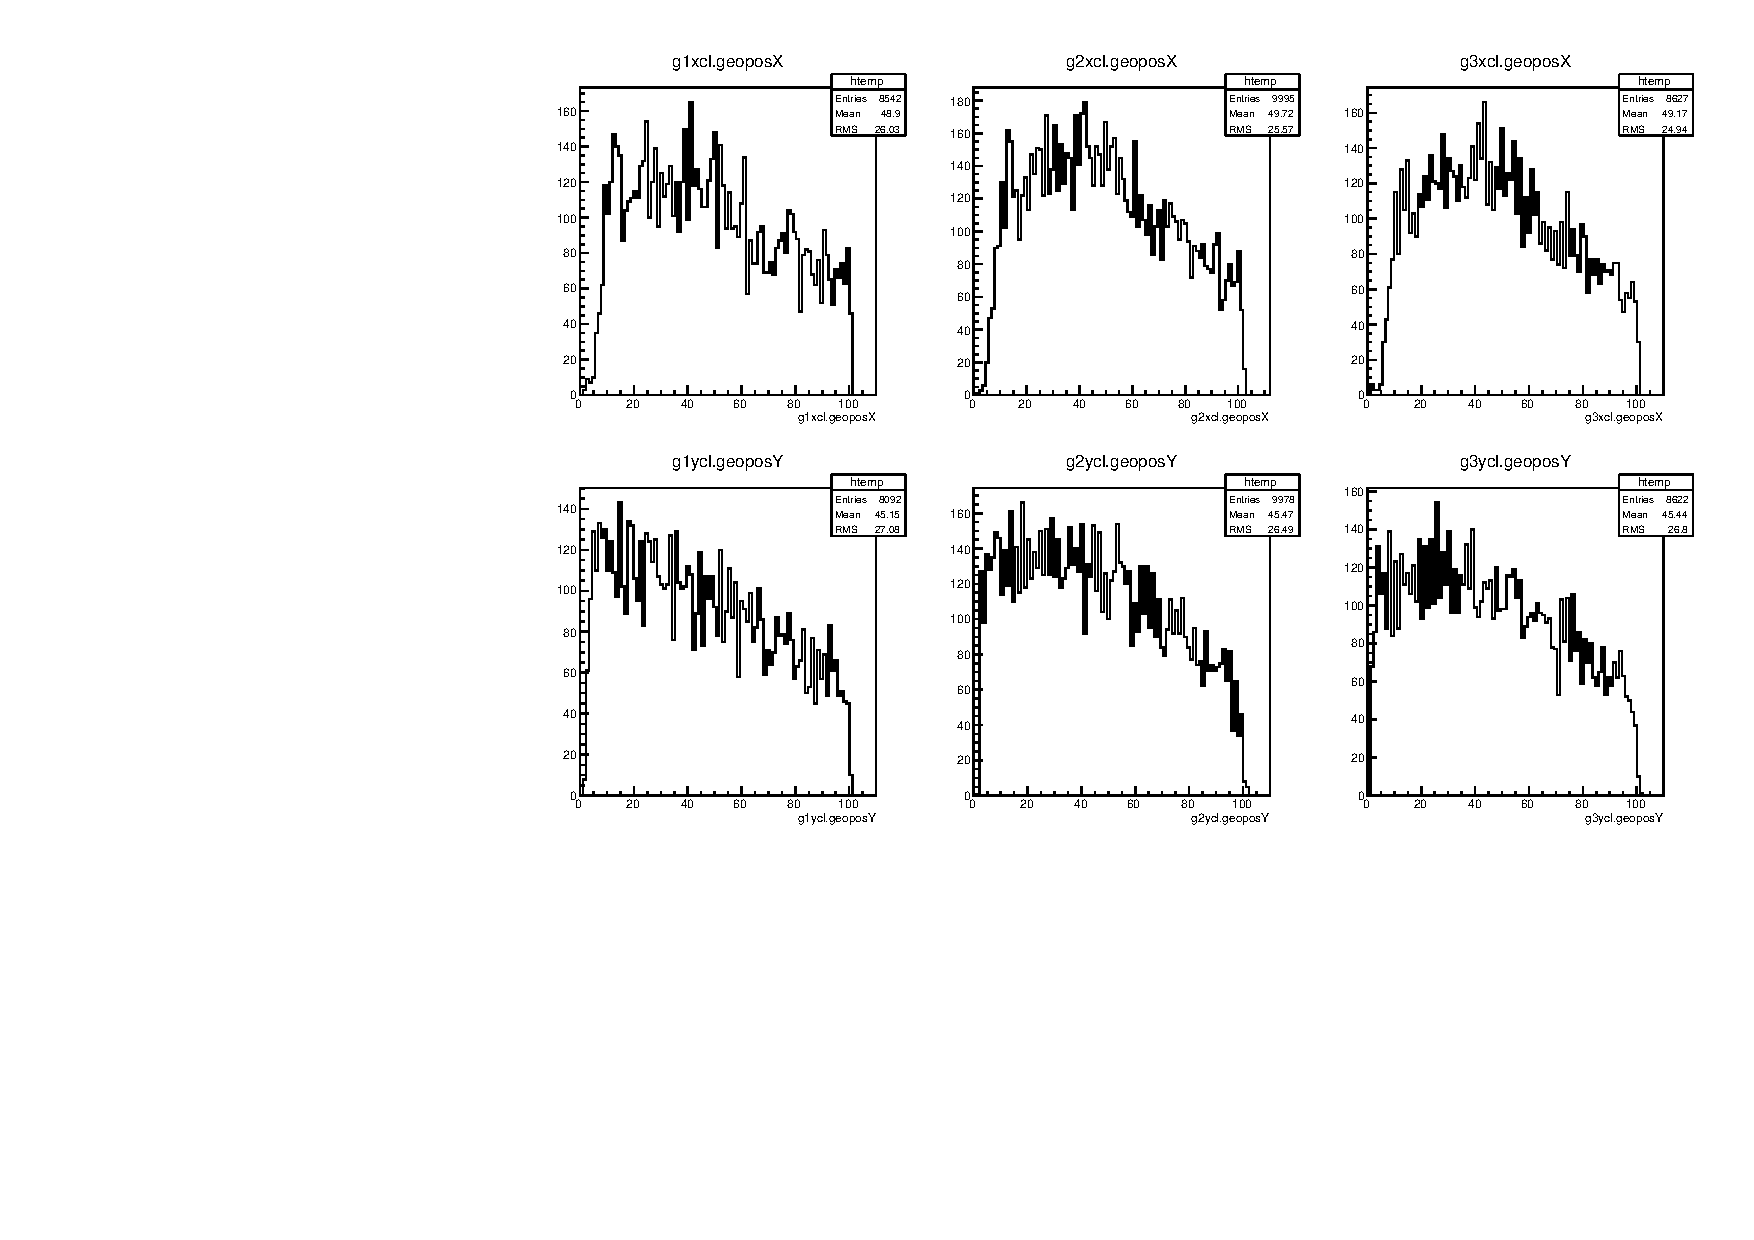
\includegraphics[width=12cm,height=8cm]{Tracker_Hit_position_1136.pdf}
%         };
%         \draw (2, 3) node {\color{red} };	% can comment anyting at a position 2,3
%         \end{tikzpicture}
\end{frame}
\begin{frame}\frametitle{Tracker Hit position 1135}
%        \begin{tikzpicture}
%         \draw (0, 0) node[inner sep=0]
 %        {
	 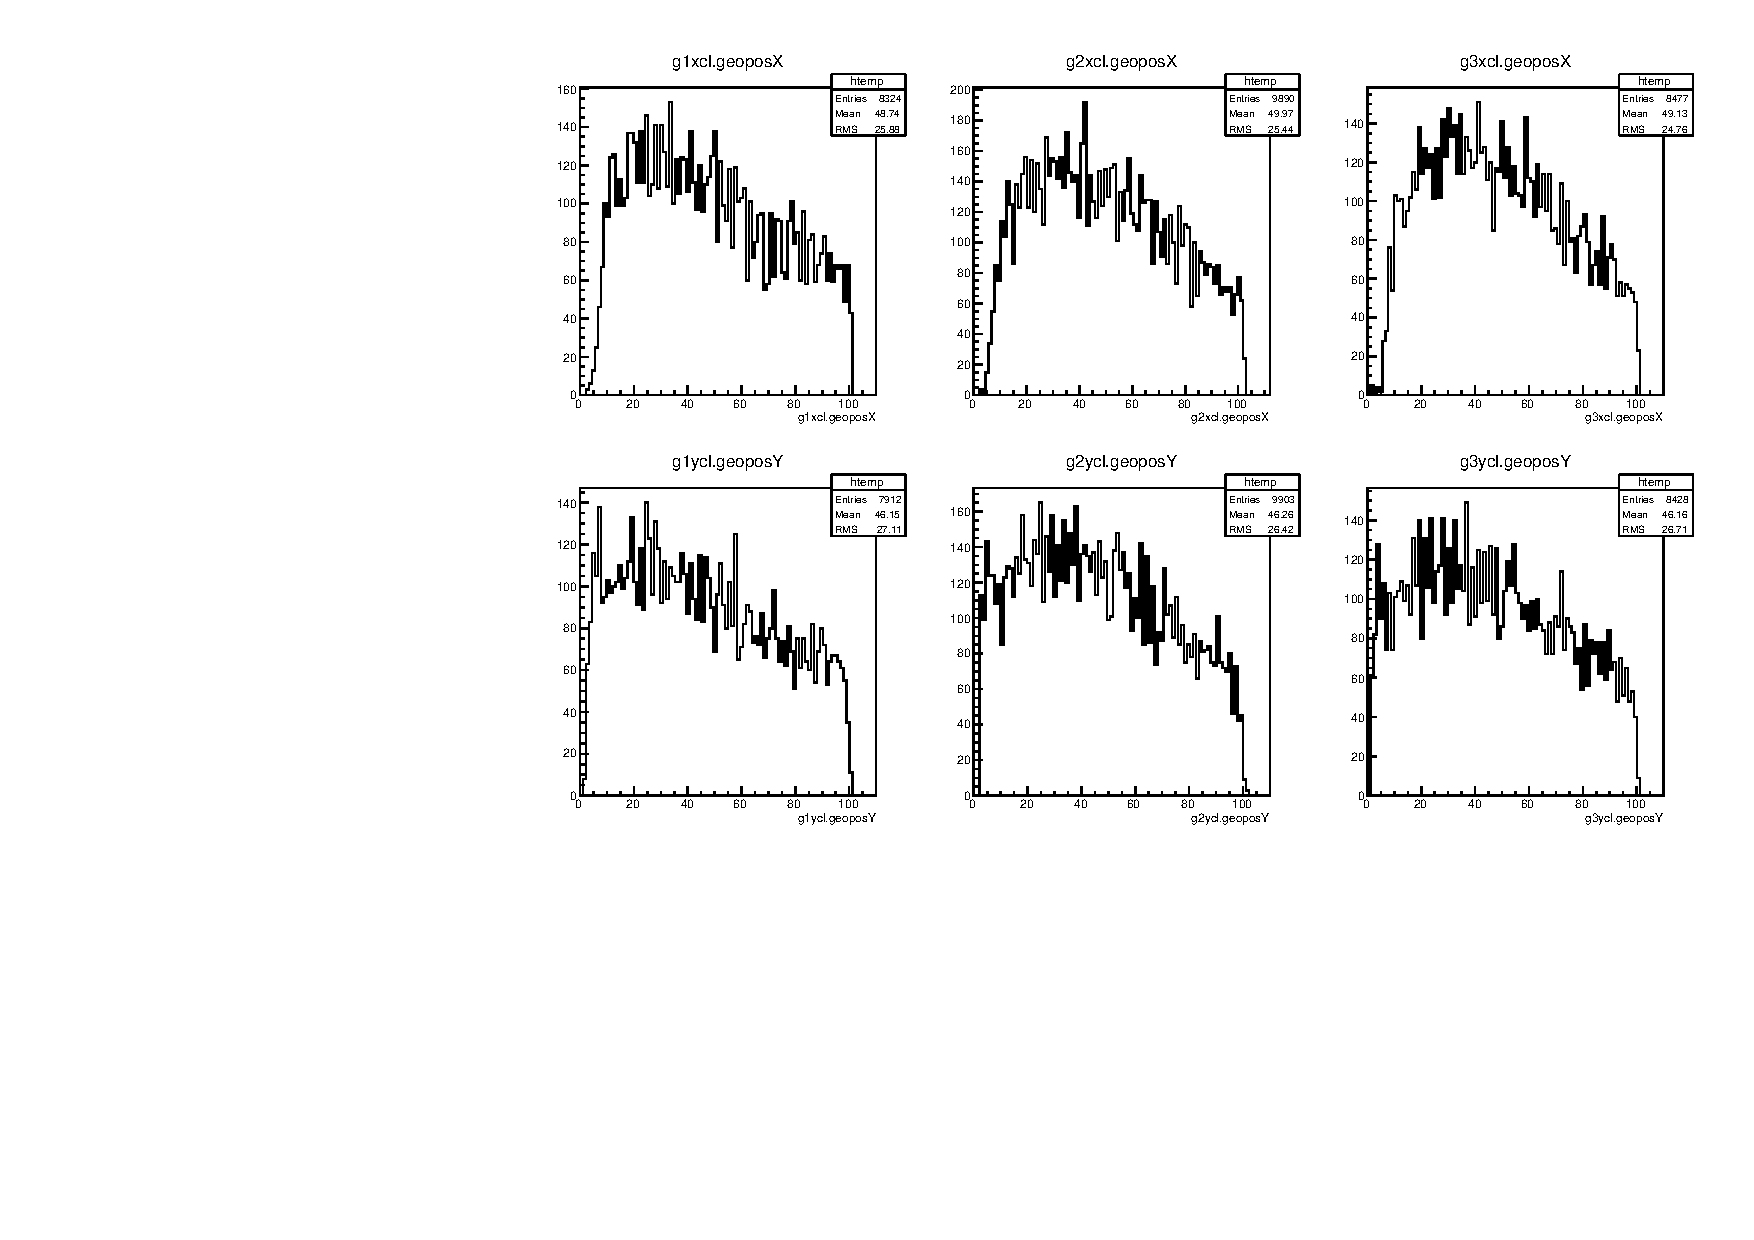
\includegraphics[width=12cm,height=8cm]{Tracker_Hit_position_1135.pdf}
%         };
%         \draw (2, 3) node {\color{red} };	% can comment anyting at a position 2,3
%         \end{tikzpicture}
\end{frame}
\begin{frame}\frametitle{Tracker Hit position 1134}
%        \begin{tikzpicture}
%         \draw (0, 0) node[inner sep=0]
 %        {
	 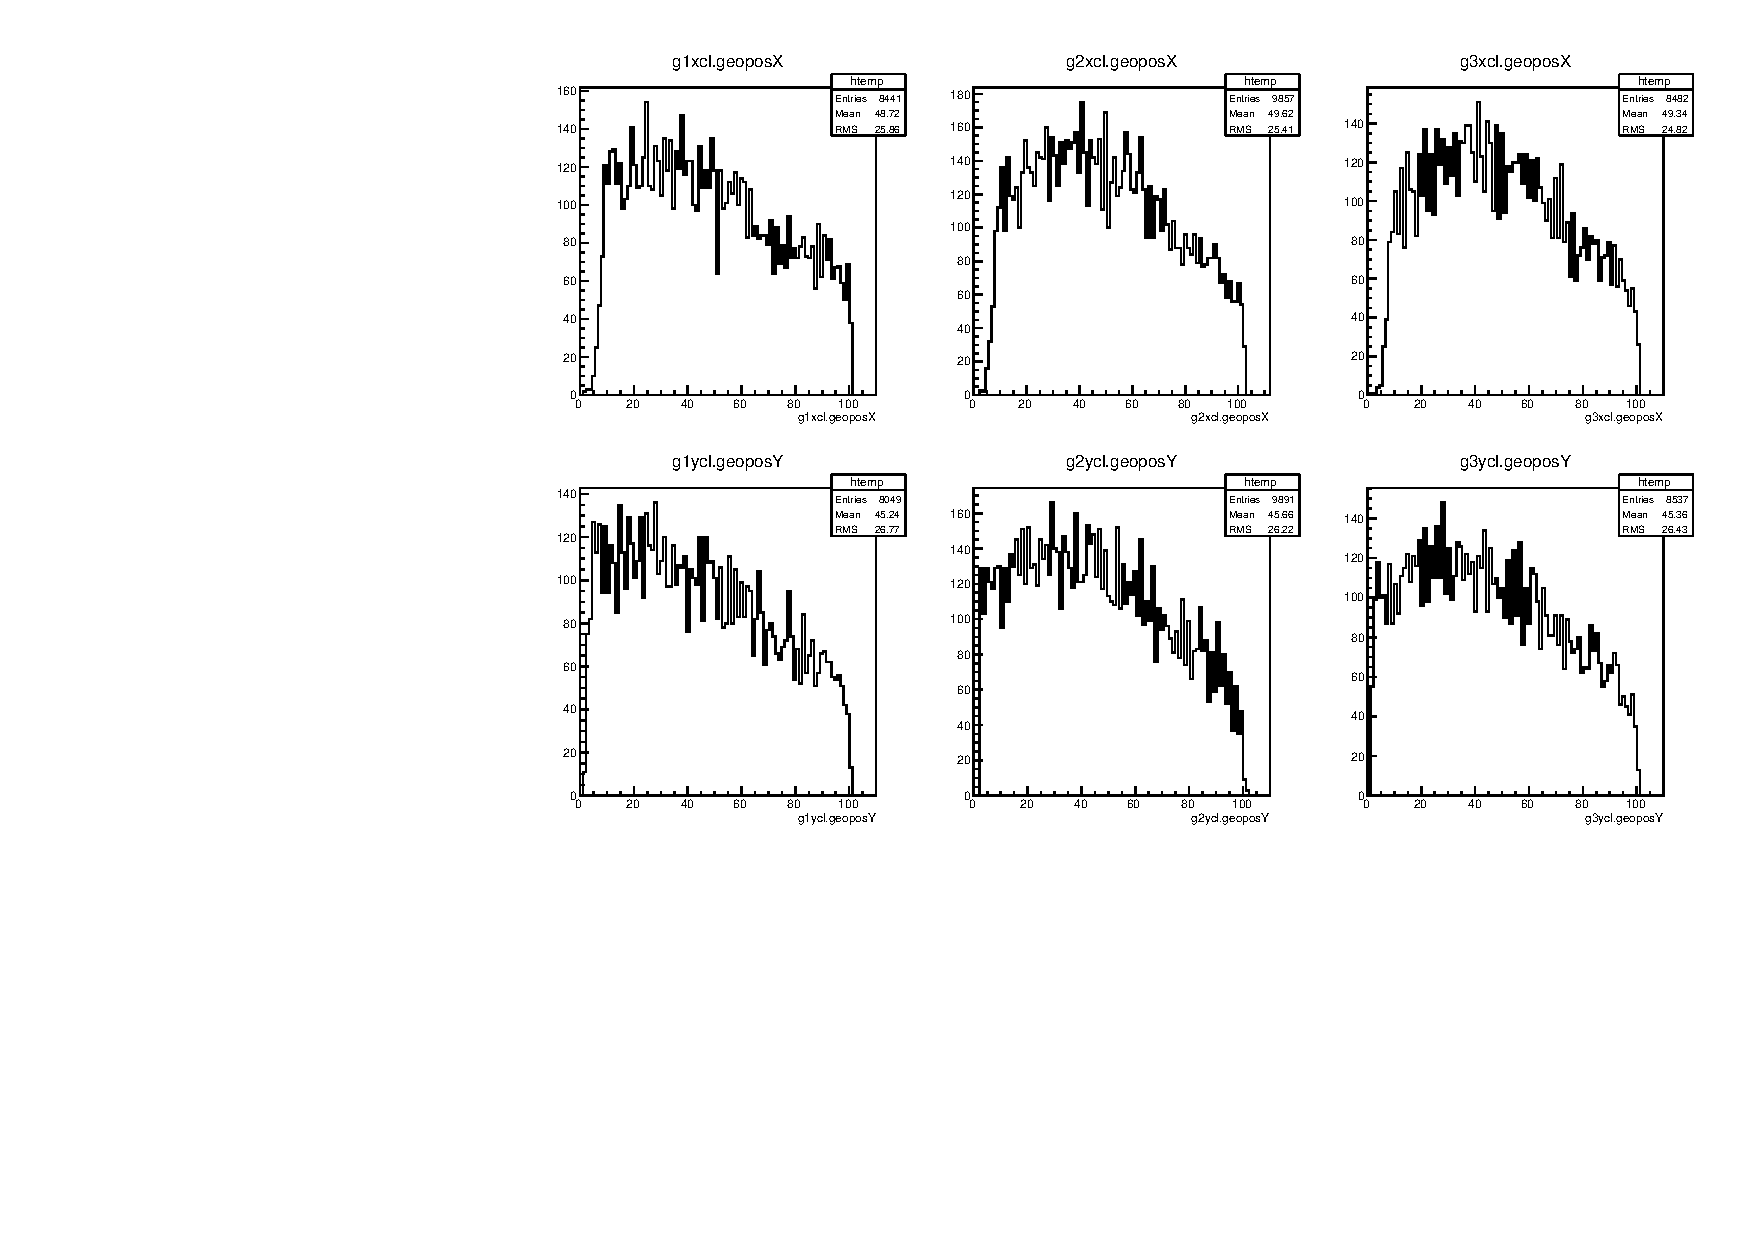
\includegraphics[width=12cm,height=8cm]{Tracker_Hit_position_1134.pdf}
%         };
%         \draw (2, 3) node {\color{red} };	% can comment anyting at a position 2,3
%         \end{tikzpicture}
\end{frame}
\begin{frame}\frametitle{Tracker Hit position 1133}
%        \begin{tikzpicture}
%         \draw (0, 0) node[inner sep=0]
 %        {
	 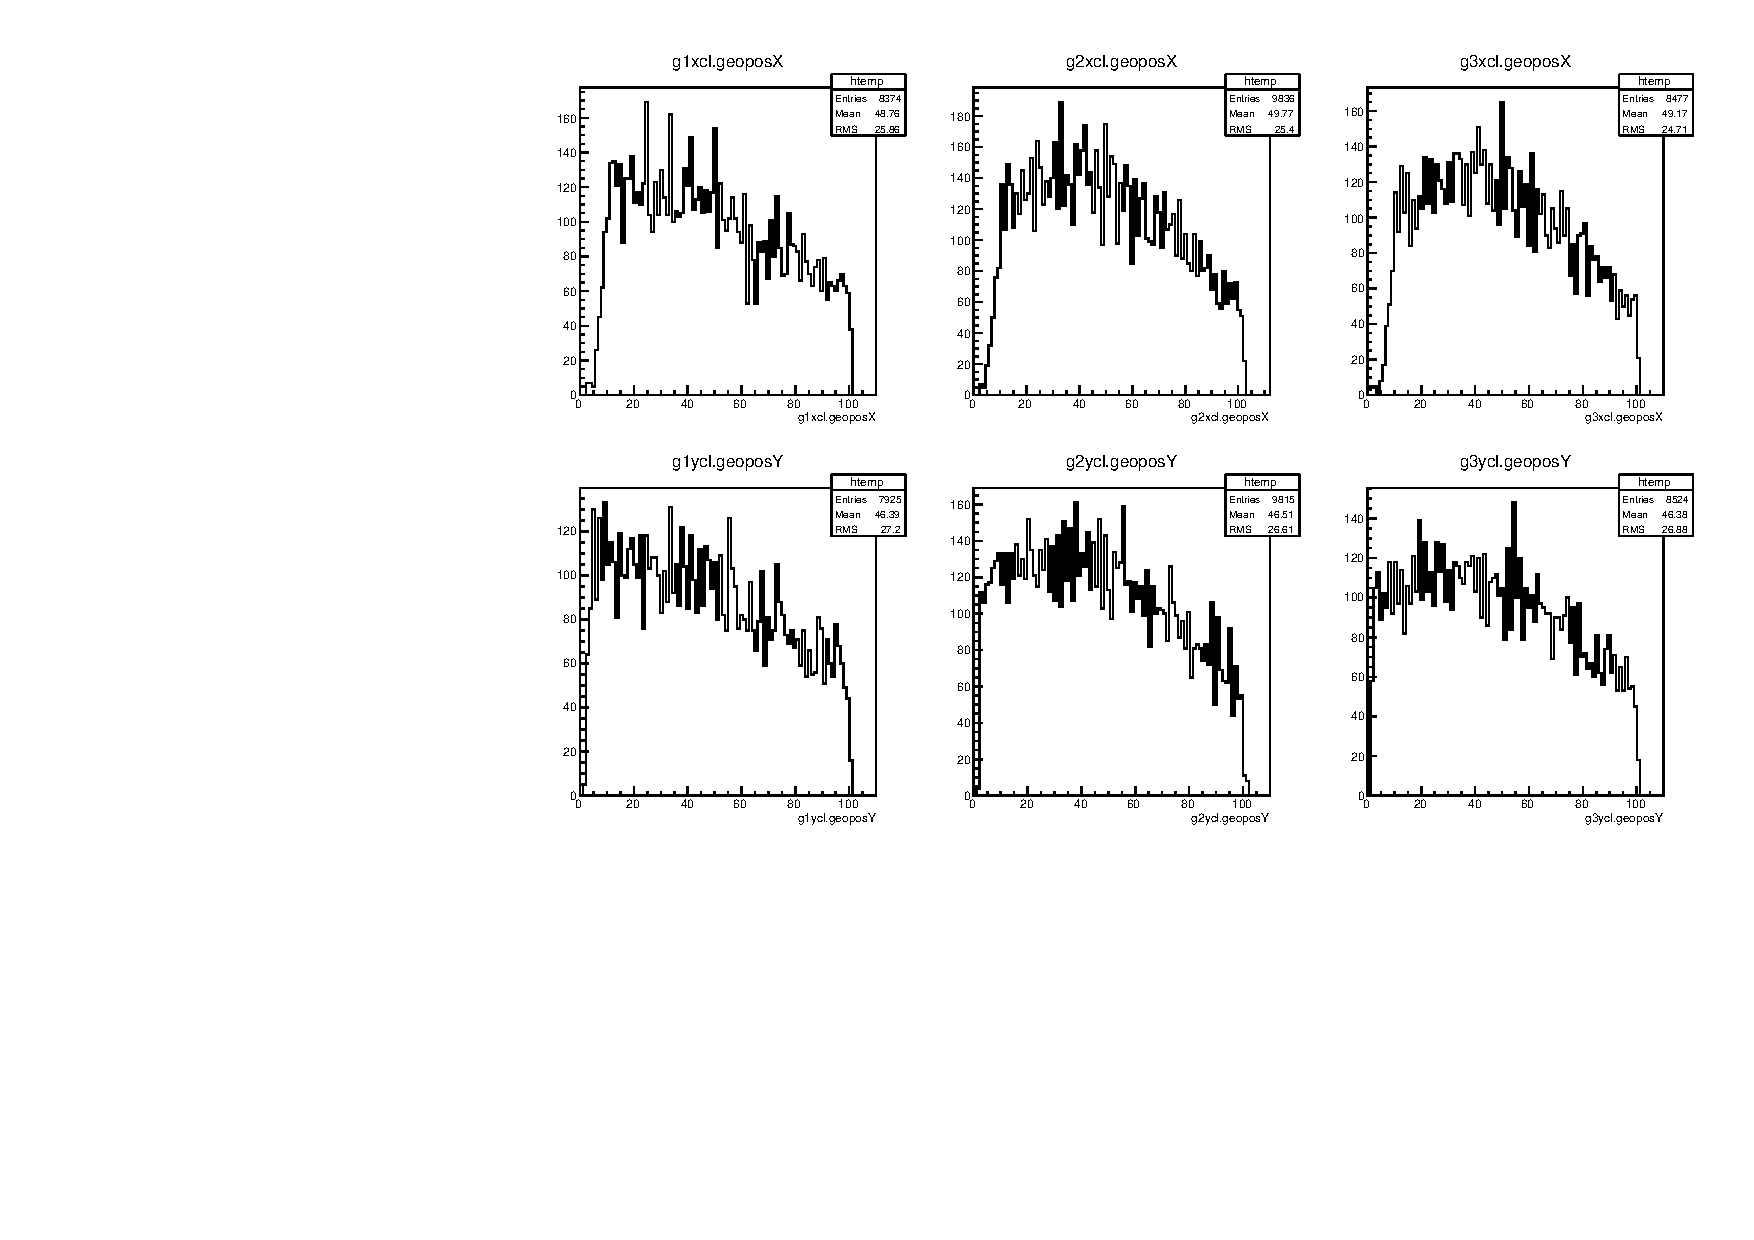
\includegraphics[width=12cm,height=8cm]{Tracker_Hit_position_1133.pdf}
%         };
%         \draw (2, 3) node {\color{red} };	% can comment anyting at a position 2,3
%         \end{tikzpicture}
\end{frame}
\begin{frame}\frametitle{Tracker Hit position 1132}
%        \begin{tikzpicture}
%         \draw (0, 0) node[inner sep=0]
 %        {
	 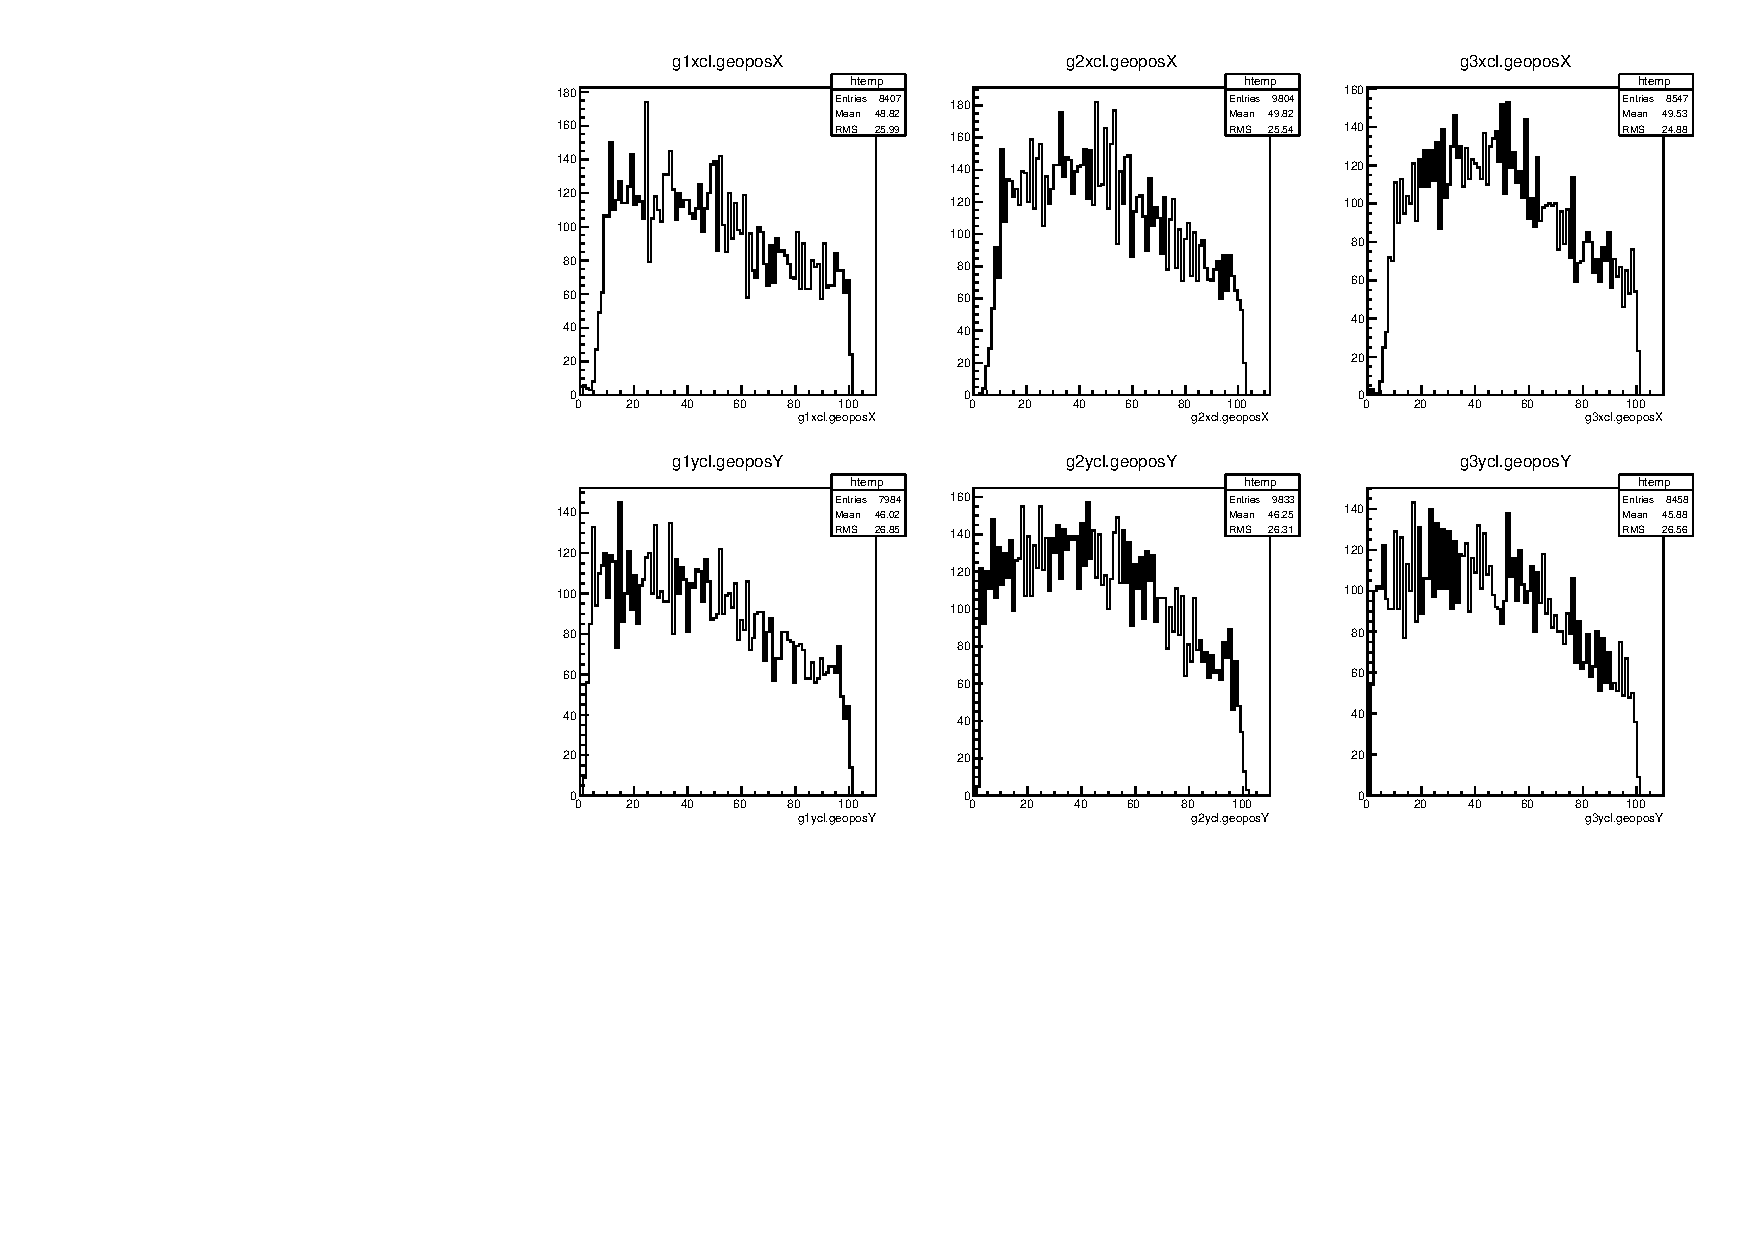
\includegraphics[width=12cm,height=8cm]{Tracker_Hit_position_1132.pdf}
%         };
%         \draw (2, 3) node {\color{red} };	% can comment anyting at a position 2,3
%         \end{tikzpicture}
\end{frame}
\begin{frame}\frametitle{Tracker Hit position 1131}
%        \begin{tikzpicture}
%         \draw (0, 0) node[inner sep=0]
 %        {
	 
\includegraphics[width=12cm,height=8cm]{Tracker_Hit_position_1131.pdf}
%         };
%         \draw (2, 3) node {\color{red} };	% can comment anyting at a position 2,3
%         \end{tikzpicture}
\end{frame}
\begin{frame}\frametitle{Tracker Hit position 1130}
%        \begin{tikzpicture}
%         \draw (0, 0) node[inner sep=0]
 %        {
	 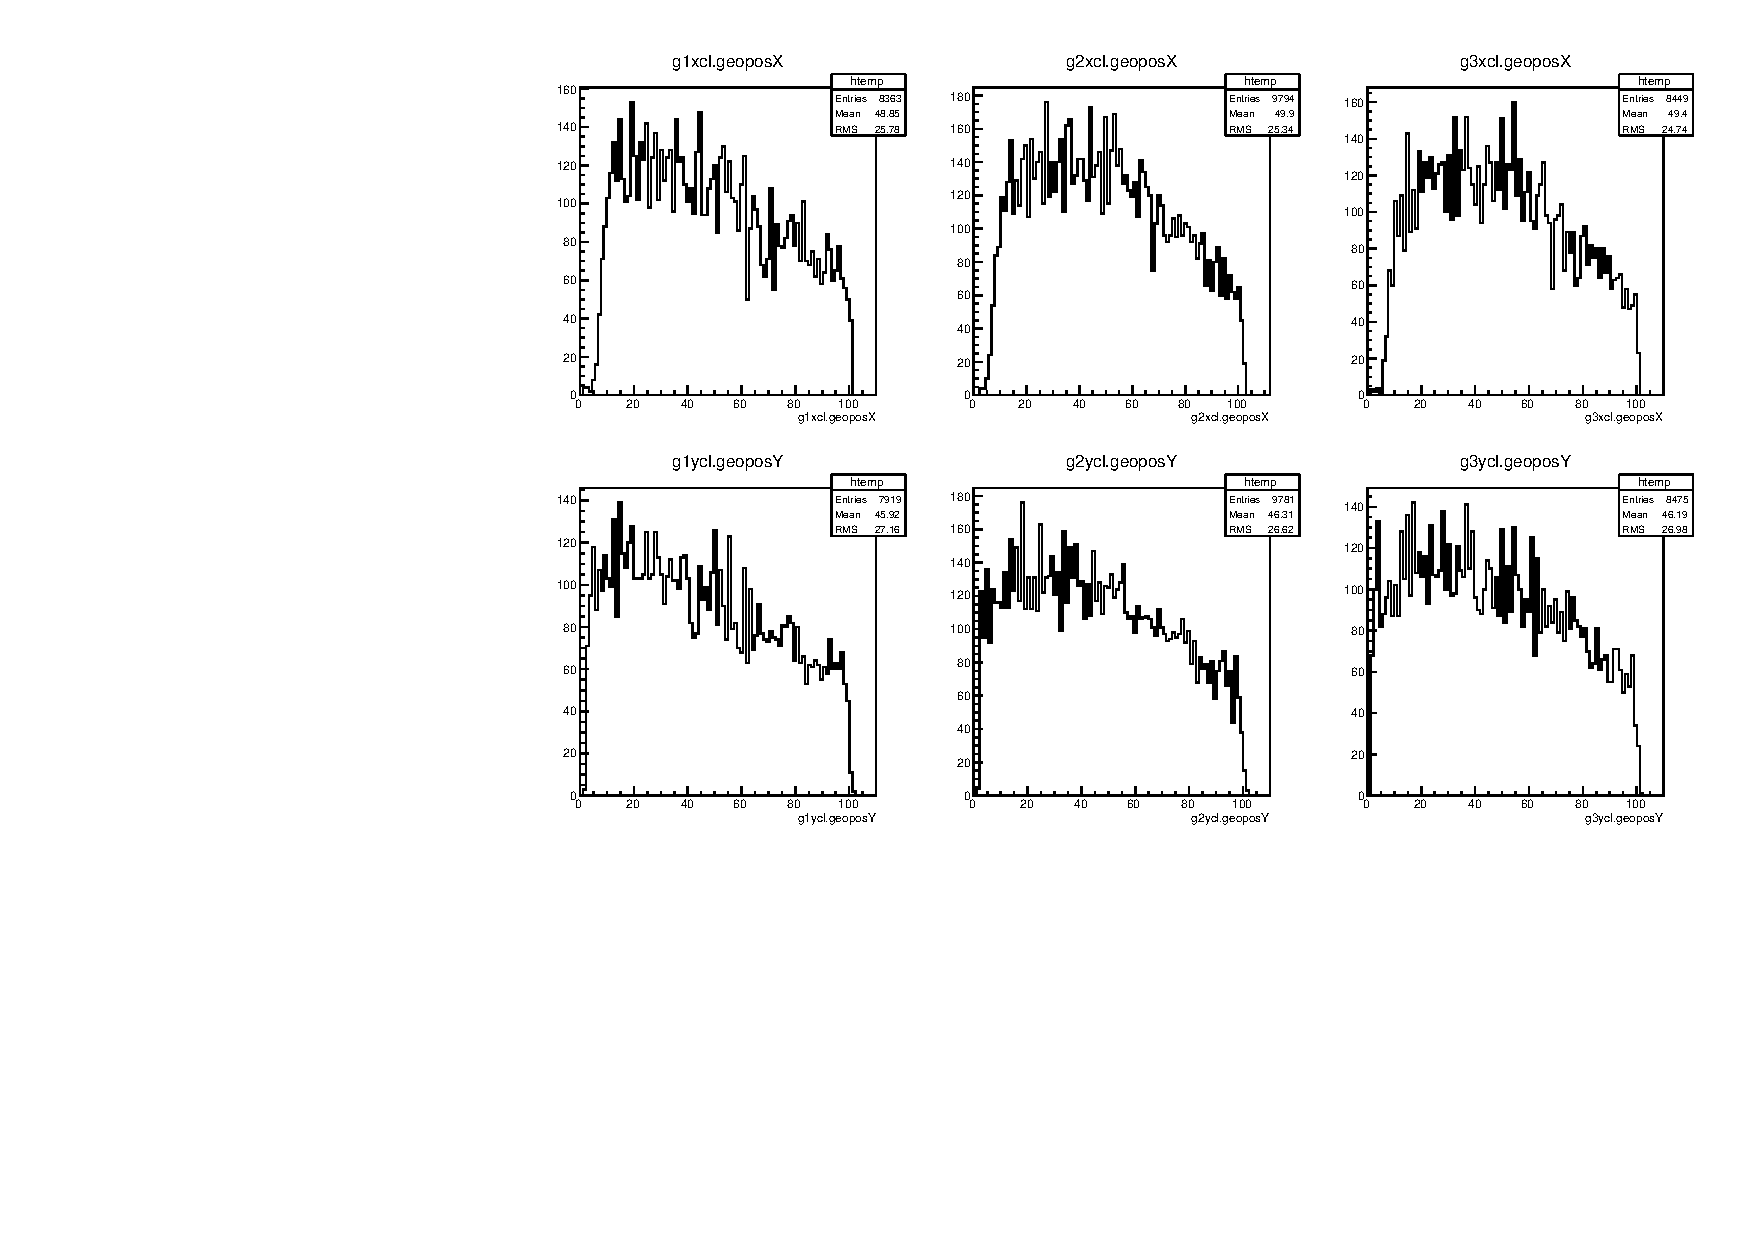
\includegraphics[width=12cm,height=8cm]{Tracker_Hit_position_1130.pdf}
%         };
%         \draw (2, 3) node {\color{red} };	% can comment anyting at a position 2,3
%         \end{tikzpicture}
\end{frame}
\begin{frame}\frametitle{Tracker Hit position 1129}
%        \begin{tikzpicture}
%         \draw (0, 0) node[inner sep=0]
 %        {
	 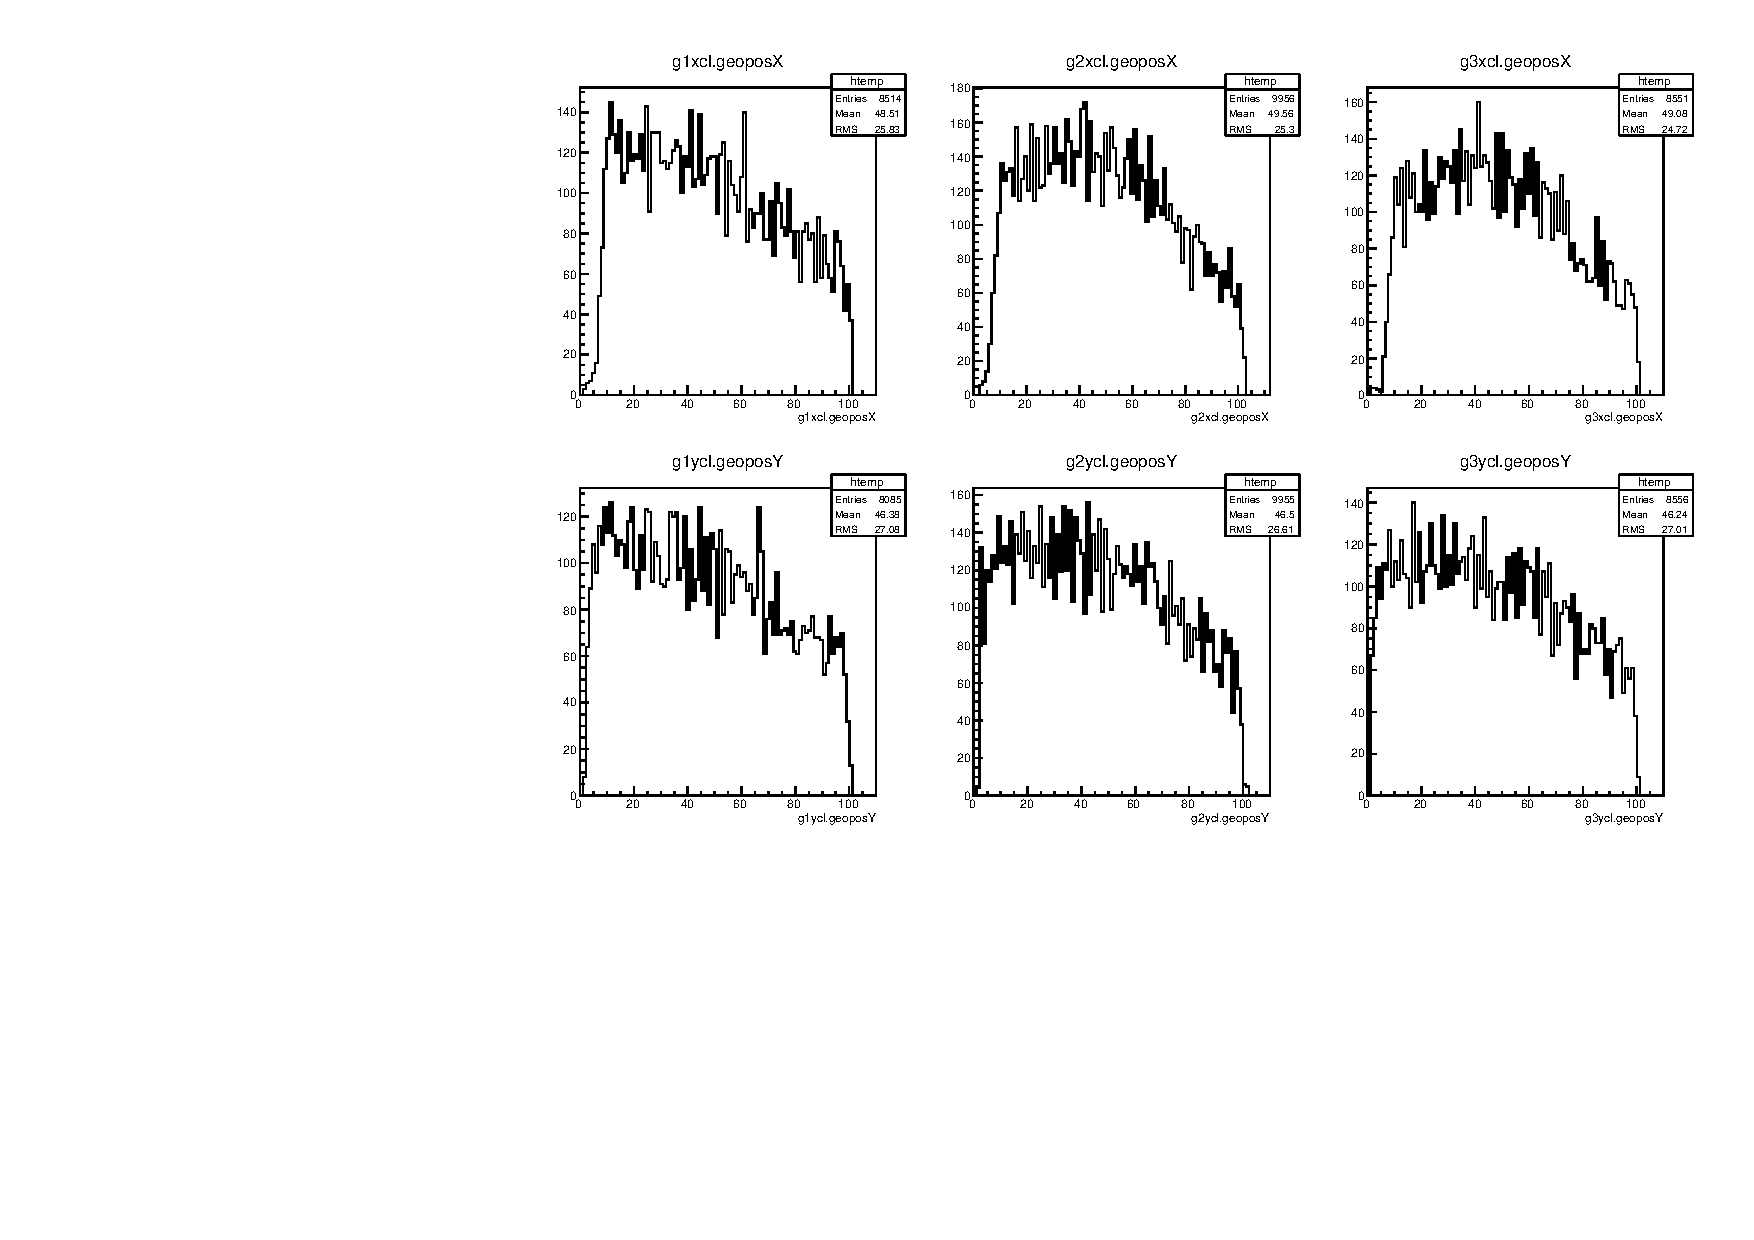
\includegraphics[width=12cm,height=8cm]{Tracker_Hit_position_1129.pdf}
%         };
%         \draw (2, 3) node {\color{red} };	% can comment anyting at a position 2,3
%         \end{tikzpicture}
\end{frame}
\begin{frame}\frametitle{Tracker Hit position 1128}
%        \begin{tikzpicture}
%         \draw (0, 0) node[inner sep=0]
 %        {
	 \includegraphics[width=12cm,height=8cm]{Tracker_Hit_position_1128.pdf}
%         };
%         \draw (2, 3) node {\color{red} };	% can comment anyting at a position 2,3
%         \end{tikzpicture}
\end{frame}
\begin{frame}\frametitle{Tracker Hit position 1127}
%        \begin{tikzpicture}
%         \draw (0, 0) node[inner sep=0]
 %        {
	 \includegraphics[width=12cm,height=8cm]{Tracker_Hit_position_1127.pdf}
%         };
%         \draw (2, 3) node {\color{red} };	% can comment anyting at a position 2,3
%         \end{tikzpicture}
\end{frame}
\begin{frame}\frametitle{Tracker Hit position 1126}
%        \begin{tikzpicture}
%         \draw (0, 0) node[inner sep=0]
 %        {
	 \includegraphics[width=12cm,height=8cm]{Tracker_Hit_position_1126.pdf}
%         };
%         \draw (2, 3) node {\color{red} };	% can comment anyting at a position 2,3
%         \end{tikzpicture}
\end{frame}
\begin{frame}\frametitle{Tracker Hit position 1125}
%        \begin{tikzpicture}
%         \draw (0, 0) node[inner sep=0]
 %        {
	 \includegraphics[width=12cm,height=8cm]{Tracker_Hit_position_1125.pdf}
%         };
%         \draw (2, 3) node {\color{red} };	% can comment anyting at a position 2,3
%         \end{tikzpicture}
\end{frame}
\begin{frame}\frametitle{Tracker Hit position 1124}
%        \begin{tikzpicture}
%         \draw (0, 0) node[inner sep=0]
 %        {
	 \includegraphics[width=12cm,height=8cm]{Tracker_Hit_position_1124.pdf}
%         };
%         \draw (2, 3) node {\color{red} };	% can comment anyting at a position 2,3
%         \end{tikzpicture}
\end{frame}
\begin{frame}\frametitle{Tracker Hit position 1123}
%        \begin{tikzpicture}
%         \draw (0, 0) node[inner sep=0]
 %        {
	 \includegraphics[width=12cm,height=8cm]{Tracker_Hit_position_1123.pdf}
%         };
%         \draw (2, 3) node {\color{red} };	% can comment anyting at a position 2,3
%         \end{tikzpicture}
\end{frame}
\begin{frame}\frametitle{Tracker Hit position 1122}
%        \begin{tikzpicture}
%         \draw (0, 0) node[inner sep=0]
 %        {
	 \includegraphics[width=12cm,height=8cm]{Tracker_Hit_position_1122.pdf}
%         };
%         \draw (2, 3) node {\color{red} };	% can comment anyting at a position 2,3
%         \end{tikzpicture}
\end{frame}
\begin{frame}\frametitle{Tracker Hit position 1121}
%        \begin{tikzpicture}
%         \draw (0, 0) node[inner sep=0]
 %        {
	 \includegraphics[width=12cm,height=8cm]{Tracker_Hit_position_1121.pdf}
%         };
%         \draw (2, 3) node {\color{red} };	% can comment anyting at a position 2,3
%         \end{tikzpicture}
\end{frame}
\begin{frame}\frametitle{Tracker Hit position 1120}
%        \begin{tikzpicture}
%         \draw (0, 0) node[inner sep=0]
 %        {
	 \includegraphics[width=12cm,height=8cm]{Tracker_Hit_position_1120.pdf}
%         };
%         \draw (2, 3) node {\color{red} };	% can comment anyting at a position 2,3
%         \end{tikzpicture}
\end{frame}
\begin{frame}\frametitle{Tracker Hit position 1119}
%        \begin{tikzpicture}
%         \draw (0, 0) node[inner sep=0]
 %        {
	 \includegraphics[width=12cm,height=8cm]{Tracker_Hit_position_1119.pdf}
%         };
%         \draw (2, 3) node {\color{red} };	% can comment anyting at a position 2,3
%         \end{tikzpicture}
\end{frame}
\begin{frame}\frametitle{Tracker Hit position 1118}
%        \begin{tikzpicture}
%         \draw (0, 0) node[inner sep=0]
 %        {
	 \includegraphics[width=12cm,height=8cm]{Tracker_Hit_position_1118.pdf}
%         };
%         \draw (2, 3) node {\color{red} };	% can comment anyting at a position 2,3
%         \end{tikzpicture}
\end{frame}
\begin{frame}\frametitle{profile plots for Trackers 1187}
%        \begin{tikzpicture}
%         \draw (0, 0) node[inner sep=0]
 %        {
	 \includegraphics[width=12cm,height=8cm]{profile_plots_for_Trackers_1187.pdf}
%         };
%         \draw (2, 3) node {\color{red} };	% can comment anyting at a position 2,3
%         \end{tikzpicture}
\end{frame}
\begin{frame}\frametitle{profile plots for Trackers 1184}
%        \begin{tikzpicture}
%         \draw (0, 0) node[inner sep=0]
 %        {
	 \includegraphics[width=12cm,height=8cm]{profile_plots_for_Trackers_1184.pdf}
%         };
%         \draw (2, 3) node {\color{red} };	% can comment anyting at a position 2,3
%         \end{tikzpicture}
\end{frame}
\begin{frame}\frametitle{profile plots for Trackers 1183}
%        \begin{tikzpicture}
%         \draw (0, 0) node[inner sep=0]
 %        {
	 \includegraphics[width=12cm,height=8cm]{profile_plots_for_Trackers_1183.pdf}
%         };
%         \draw (2, 3) node {\color{red} };	% can comment anyting at a position 2,3
%         \end{tikzpicture}
\end{frame}
\begin{frame}\frametitle{profile plots for Trackers 1182}
%        \begin{tikzpicture}
%         \draw (0, 0) node[inner sep=0]
 %        {
	 \includegraphics[width=12cm,height=8cm]{profile_plots_for_Trackers_1182.pdf}
%         };
%         \draw (2, 3) node {\color{red} };	% can comment anyting at a position 2,3
%         \end{tikzpicture}
\end{frame}
\begin{frame}\frametitle{profile plots for Trackers 1181}
%        \begin{tikzpicture}
%         \draw (0, 0) node[inner sep=0]
 %        {
	 \includegraphics[width=12cm,height=8cm]{profile_plots_for_Trackers_1181.pdf}
%         };
%         \draw (2, 3) node {\color{red} };	% can comment anyting at a position 2,3
%         \end{tikzpicture}
\end{frame}
\begin{frame}\frametitle{profile plots for Trackers 1180}
%        \begin{tikzpicture}
%         \draw (0, 0) node[inner sep=0]
 %        {
	 \includegraphics[width=12cm,height=8cm]{profile_plots_for_Trackers_1180.pdf}
%         };
%         \draw (2, 3) node {\color{red} };	% can comment anyting at a position 2,3
%         \end{tikzpicture}
\end{frame}
\begin{frame}\frametitle{profile plots for Trackers 1179}
%        \begin{tikzpicture}
%         \draw (0, 0) node[inner sep=0]
 %        {
	 \includegraphics[width=12cm,height=8cm]{profile_plots_for_Trackers_1179.pdf}
%         };
%         \draw (2, 3) node {\color{red} };	% can comment anyting at a position 2,3
%         \end{tikzpicture}
\end{frame}
\begin{frame}\frametitle{profile plots for Trackers 1178}
%        \begin{tikzpicture}
%         \draw (0, 0) node[inner sep=0]
 %        {
	 \includegraphics[width=12cm,height=8cm]{profile_plots_for_Trackers_1178.pdf}
%         };
%         \draw (2, 3) node {\color{red} };	% can comment anyting at a position 2,3
%         \end{tikzpicture}
\end{frame}
\begin{frame}\frametitle{profile plots for Trackers 1174}
%        \begin{tikzpicture}
%         \draw (0, 0) node[inner sep=0]
 %        {
	 \includegraphics[width=12cm,height=8cm]{profile_plots_for_Trackers_1174.pdf}
%         };
%         \draw (2, 3) node {\color{red} };	% can comment anyting at a position 2,3
%         \end{tikzpicture}
\end{frame}
\begin{frame}\frametitle{profile plots for Trackers 1173}
%        \begin{tikzpicture}
%         \draw (0, 0) node[inner sep=0]
 %        {
	 \includegraphics[width=12cm,height=8cm]{profile_plots_for_Trackers_1173.pdf}
%         };
%         \draw (2, 3) node {\color{red} };	% can comment anyting at a position 2,3
%         \end{tikzpicture}
\end{frame}
\begin{frame}\frametitle{profile plots for Trackers 1172}
%        \begin{tikzpicture}
%         \draw (0, 0) node[inner sep=0]
 %        {
	 \includegraphics[width=12cm,height=8cm]{profile_plots_for_Trackers_1172.pdf}
%         };
%         \draw (2, 3) node {\color{red} };	% can comment anyting at a position 2,3
%         \end{tikzpicture}
\end{frame}
\begin{frame}\frametitle{profile plots for Trackers 1170}
%        \begin{tikzpicture}
%         \draw (0, 0) node[inner sep=0]
 %        {
	 \includegraphics[width=12cm,height=8cm]{profile_plots_for_Trackers_1170.pdf}
%         };
%         \draw (2, 3) node {\color{red} };	% can comment anyting at a position 2,3
%         \end{tikzpicture}
\end{frame}
\begin{frame}\frametitle{profile plots for Trackers 1168}
%        \begin{tikzpicture}
%         \draw (0, 0) node[inner sep=0]
 %        {
	 \includegraphics[width=12cm,height=8cm]{profile_plots_for_Trackers_1168.pdf}
%         };
%         \draw (2, 3) node {\color{red} };	% can comment anyting at a position 2,3
%         \end{tikzpicture}
\end{frame}
\begin{frame}\frametitle{profile plots for Trackers 1167}
%        \begin{tikzpicture}
%         \draw (0, 0) node[inner sep=0]
 %        {
	 \includegraphics[width=12cm,height=8cm]{profile_plots_for_Trackers_1167.pdf}
%         };
%         \draw (2, 3) node {\color{red} };	% can comment anyting at a position 2,3
%         \end{tikzpicture}
\end{frame}
\begin{frame}\frametitle{profile plots for Trackers 1166}
%        \begin{tikzpicture}
%         \draw (0, 0) node[inner sep=0]
 %        {
	 \includegraphics[width=12cm,height=8cm]{profile_plots_for_Trackers_1166.pdf}
%         };
%         \draw (2, 3) node {\color{red} };	% can comment anyting at a position 2,3
%         \end{tikzpicture}
\end{frame}
\begin{frame}\frametitle{profile plots for Trackers 1165}
%        \begin{tikzpicture}
%         \draw (0, 0) node[inner sep=0]
 %        {
	 \includegraphics[width=12cm,height=8cm]{profile_plots_for_Trackers_1165.pdf}
%         };
%         \draw (2, 3) node {\color{red} };	% can comment anyting at a position 2,3
%         \end{tikzpicture}
\end{frame}
\begin{frame}\frametitle{profile plots for Trackers 1164}
%        \begin{tikzpicture}
%         \draw (0, 0) node[inner sep=0]
 %        {
	 \includegraphics[width=12cm,height=8cm]{profile_plots_for_Trackers_1164.pdf}
%         };
%         \draw (2, 3) node {\color{red} };	% can comment anyting at a position 2,3
%         \end{tikzpicture}
\end{frame}
\begin{frame}\frametitle{profile plots for Trackers 1163}
%        \begin{tikzpicture}
%         \draw (0, 0) node[inner sep=0]
 %        {
	 \includegraphics[width=12cm,height=8cm]{profile_plots_for_Trackers_1163.pdf}
%         };
%         \draw (2, 3) node {\color{red} };	% can comment anyting at a position 2,3
%         \end{tikzpicture}
\end{frame}
\begin{frame}\frametitle{profile plots for Trackers 1158}
%        \begin{tikzpicture}
%         \draw (0, 0) node[inner sep=0]
 %        {
	 \includegraphics[width=12cm,height=8cm]{profile_plots_for_Trackers_1158.pdf}
%         };
%         \draw (2, 3) node {\color{red} };	% can comment anyting at a position 2,3
%         \end{tikzpicture}
\end{frame}
\begin{frame}\frametitle{profile plots for Trackers 1157}
%        \begin{tikzpicture}
%         \draw (0, 0) node[inner sep=0]
 %        {
	 \includegraphics[width=12cm,height=8cm]{profile_plots_for_Trackers_1157.pdf}
%         };
%         \draw (2, 3) node {\color{red} };	% can comment anyting at a position 2,3
%         \end{tikzpicture}
\end{frame}
\begin{frame}\frametitle{profile plots for Trackers 1156}
%        \begin{tikzpicture}
%         \draw (0, 0) node[inner sep=0]
 %        {
	 \includegraphics[width=12cm,height=8cm]{profile_plots_for_Trackers_1156.pdf}
%         };
%         \draw (2, 3) node {\color{red} };	% can comment anyting at a position 2,3
%         \end{tikzpicture}
\end{frame}
\begin{frame}\frametitle{profile plots for Trackers 1155}
%        \begin{tikzpicture}
%         \draw (0, 0) node[inner sep=0]
 %        {
	 \includegraphics[width=12cm,height=8cm]{profile_plots_for_Trackers_1155.pdf}
%         };
%         \draw (2, 3) node {\color{red} };	% can comment anyting at a position 2,3
%         \end{tikzpicture}
\end{frame}
\begin{frame}\frametitle{profile plots for Trackers 1154}
%        \begin{tikzpicture}
%         \draw (0, 0) node[inner sep=0]
 %        {
	 \includegraphics[width=12cm,height=8cm]{profile_plots_for_Trackers_1154.pdf}
%         };
%         \draw (2, 3) node {\color{red} };	% can comment anyting at a position 2,3
%         \end{tikzpicture}
\end{frame}
\begin{frame}\frametitle{profile plots for Trackers 1153}
%        \begin{tikzpicture}
%         \draw (0, 0) node[inner sep=0]
 %        {
	 \includegraphics[width=12cm,height=8cm]{profile_plots_for_Trackers_1153.pdf}
%         };
%         \draw (2, 3) node {\color{red} };	% can comment anyting at a position 2,3
%         \end{tikzpicture}
\end{frame}
\begin{frame}\frametitle{profile plots for Trackers 1152}
%        \begin{tikzpicture}
%         \draw (0, 0) node[inner sep=0]
 %        {
	 \includegraphics[width=12cm,height=8cm]{profile_plots_for_Trackers_1152.pdf}
%         };
%         \draw (2, 3) node {\color{red} };	% can comment anyting at a position 2,3
%         \end{tikzpicture}
\end{frame}
\begin{frame}\frametitle{profile plots for Trackers 1151}
%        \begin{tikzpicture}
%         \draw (0, 0) node[inner sep=0]
 %        {
	 \includegraphics[width=12cm,height=8cm]{profile_plots_for_Trackers_1151.pdf}
%         };
%         \draw (2, 3) node {\color{red} };	% can comment anyting at a position 2,3
%         \end{tikzpicture}
\end{frame}
\begin{frame}\frametitle{profile plots for Trackers 1150}
%        \begin{tikzpicture}
%         \draw (0, 0) node[inner sep=0]
 %        {
	 \includegraphics[width=12cm,height=8cm]{profile_plots_for_Trackers_1150.pdf}
%         };
%         \draw (2, 3) node {\color{red} };	% can comment anyting at a position 2,3
%         \end{tikzpicture}
\end{frame}
\begin{frame}\frametitle{profile plots for Trackers 1149}
%        \begin{tikzpicture}
%         \draw (0, 0) node[inner sep=0]
 %        {
	 \includegraphics[width=12cm,height=8cm]{profile_plots_for_Trackers_1149.pdf}
%         };
%         \draw (2, 3) node {\color{red} };	% can comment anyting at a position 2,3
%         \end{tikzpicture}
\end{frame}
\begin{frame}\frametitle{profile plots for Trackers 1147}
%        \begin{tikzpicture}
%         \draw (0, 0) node[inner sep=0]
 %        {
	 \includegraphics[width=12cm,height=8cm]{profile_plots_for_Trackers_1147.pdf}
%         };
%         \draw (2, 3) node {\color{red} };	% can comment anyting at a position 2,3
%         \end{tikzpicture}
\end{frame}
\begin{frame}\frametitle{profile plots for Trackers 1146}
%        \begin{tikzpicture}
%         \draw (0, 0) node[inner sep=0]
 %        {
	 \includegraphics[width=12cm,height=8cm]{profile_plots_for_Trackers_1146.pdf}
%         };
%         \draw (2, 3) node {\color{red} };	% can comment anyting at a position 2,3
%         \end{tikzpicture}
\end{frame}
\begin{frame}\frametitle{profile plots for Trackers 1145}
%        \begin{tikzpicture}
%         \draw (0, 0) node[inner sep=0]
 %        {
	 \includegraphics[width=12cm,height=8cm]{profile_plots_for_Trackers_1145.pdf}
%         };
%         \draw (2, 3) node {\color{red} };	% can comment anyting at a position 2,3
%         \end{tikzpicture}
\end{frame}
\begin{frame}\frametitle{profile plots for Trackers 1141}
%        \begin{tikzpicture}
%         \draw (0, 0) node[inner sep=0]
 %        {
	 \includegraphics[width=12cm,height=8cm]{profile_plots_for_Trackers_1141.pdf}
%         };
%         \draw (2, 3) node {\color{red} };	% can comment anyting at a position 2,3
%         \end{tikzpicture}
\end{frame}
\begin{frame}\frametitle{profile plots for Trackers 1140}
%        \begin{tikzpicture}
%         \draw (0, 0) node[inner sep=0]
 %        {
	 \includegraphics[width=12cm,height=8cm]{profile_plots_for_Trackers_1140.pdf}
%         };
%         \draw (2, 3) node {\color{red} };	% can comment anyting at a position 2,3
%         \end{tikzpicture}
\end{frame}
\begin{frame}\frametitle{profile plots for Trackers 1139}
%        \begin{tikzpicture}
%         \draw (0, 0) node[inner sep=0]
 %        {
	 \includegraphics[width=12cm,height=8cm]{profile_plots_for_Trackers_1139.pdf}
%         };
%         \draw (2, 3) node {\color{red} };	% can comment anyting at a position 2,3
%         \end{tikzpicture}
\end{frame}
\begin{frame}\frametitle{profile plots for Trackers 1138}
%        \begin{tikzpicture}
%         \draw (0, 0) node[inner sep=0]
 %        {
	 \includegraphics[width=12cm,height=8cm]{profile_plots_for_Trackers_1138.pdf}
%         };
%         \draw (2, 3) node {\color{red} };	% can comment anyting at a position 2,3
%         \end{tikzpicture}
\end{frame}
\begin{frame}\frametitle{profile plots for Trackers 1137}
%        \begin{tikzpicture}
%         \draw (0, 0) node[inner sep=0]
 %        {
	 \includegraphics[width=12cm,height=8cm]{profile_plots_for_Trackers_1137.pdf}
%         };
%         \draw (2, 3) node {\color{red} };	% can comment anyting at a position 2,3
%         \end{tikzpicture}
\end{frame}
\begin{frame}\frametitle{profile plots for Trackers 1136}
%        \begin{tikzpicture}
%         \draw (0, 0) node[inner sep=0]
 %        {
	 \includegraphics[width=12cm,height=8cm]{profile_plots_for_Trackers_1136.pdf}
%         };
%         \draw (2, 3) node {\color{red} };	% can comment anyting at a position 2,3
%         \end{tikzpicture}
\end{frame}
\begin{frame}\frametitle{profile plots for Trackers 1135}
%        \begin{tikzpicture}
%         \draw (0, 0) node[inner sep=0]
 %        {
	 \includegraphics[width=12cm,height=8cm]{profile_plots_for_Trackers_1135.pdf}
%         };
%         \draw (2, 3) node {\color{red} };	% can comment anyting at a position 2,3
%         \end{tikzpicture}
\end{frame}
\begin{frame}\frametitle{profile plots for Trackers 1134}
%        \begin{tikzpicture}
%         \draw (0, 0) node[inner sep=0]
 %        {
	 \includegraphics[width=12cm,height=8cm]{profile_plots_for_Trackers_1134.pdf}
%         };
%         \draw (2, 3) node {\color{red} };	% can comment anyting at a position 2,3
%         \end{tikzpicture}
\end{frame}
\begin{frame}\frametitle{profile plots for Trackers 1133}
%        \begin{tikzpicture}
%         \draw (0, 0) node[inner sep=0]
 %        {
	 \includegraphics[width=12cm,height=8cm]{profile_plots_for_Trackers_1133.pdf}
%         };
%         \draw (2, 3) node {\color{red} };	% can comment anyting at a position 2,3
%         \end{tikzpicture}
\end{frame}
\begin{frame}\frametitle{profile plots for Trackers 1132}
%        \begin{tikzpicture}
%         \draw (0, 0) node[inner sep=0]
 %        {
	 \includegraphics[width=12cm,height=8cm]{profile_plots_for_Trackers_1132.pdf}
%         };
%         \draw (2, 3) node {\color{red} };	% can comment anyting at a position 2,3
%         \end{tikzpicture}
\end{frame}
\begin{frame}\frametitle{profile plots for Trackers 1131}
%        \begin{tikzpicture}
%         \draw (0, 0) node[inner sep=0]
 %        {
	 \includegraphics[width=12cm,height=8cm]{profile_plots_for_Trackers_1131.pdf}
%         };
%         \draw (2, 3) node {\color{red} };	% can comment anyting at a position 2,3
%         \end{tikzpicture}
\end{frame}
\begin{frame}\frametitle{profile plots for Trackers 1130}
%        \begin{tikzpicture}
%         \draw (0, 0) node[inner sep=0]
 %        {
	 \includegraphics[width=12cm,height=8cm]{profile_plots_for_Trackers_1130.pdf}
%         };
%         \draw (2, 3) node {\color{red} };	% can comment anyting at a position 2,3
%         \end{tikzpicture}
\end{frame}
\begin{frame}\frametitle{profile plots for Trackers 1129}
%        \begin{tikzpicture}
%         \draw (0, 0) node[inner sep=0]
 %        {
	 \includegraphics[width=12cm,height=8cm]{profile_plots_for_Trackers_1129.pdf}
%         };
%         \draw (2, 3) node {\color{red} };	% can comment anyting at a position 2,3
%         \end{tikzpicture}
\end{frame}
\begin{frame}\frametitle{profile plots for Trackers 1128}
%        \begin{tikzpicture}
%         \draw (0, 0) node[inner sep=0]
 %        {
	 \includegraphics[width=12cm,height=8cm]{profile_plots_for_Trackers_1128.pdf}
%         };
%         \draw (2, 3) node {\color{red} };	% can comment anyting at a position 2,3
%         \end{tikzpicture}
\end{frame}
\begin{frame}\frametitle{profile plots for Trackers 1127}
%        \begin{tikzpicture}
%         \draw (0, 0) node[inner sep=0]
 %        {
	 \includegraphics[width=12cm,height=8cm]{profile_plots_for_Trackers_1127.pdf}
%         };
%         \draw (2, 3) node {\color{red} };	% can comment anyting at a position 2,3
%         \end{tikzpicture}
\end{frame}
\begin{frame}\frametitle{profile plots for Trackers 1126}
%        \begin{tikzpicture}
%         \draw (0, 0) node[inner sep=0]
 %        {
	 \includegraphics[width=12cm,height=8cm]{profile_plots_for_Trackers_1126.pdf}
%         };
%         \draw (2, 3) node {\color{red} };	% can comment anyting at a position 2,3
%         \end{tikzpicture}
\end{frame}
\begin{frame}\frametitle{profile plots for Trackers 1125}
%        \begin{tikzpicture}
%         \draw (0, 0) node[inner sep=0]
 %        {
	 \includegraphics[width=12cm,height=8cm]{profile_plots_for_Trackers_1125.pdf}
%         };
%         \draw (2, 3) node {\color{red} };	% can comment anyting at a position 2,3
%         \end{tikzpicture}
\end{frame}
\begin{frame}\frametitle{profile plots for Trackers 1124}
%        \begin{tikzpicture}
%         \draw (0, 0) node[inner sep=0]
 %        {
	 \includegraphics[width=12cm,height=8cm]{profile_plots_for_Trackers_1124.pdf}
%         };
%         \draw (2, 3) node {\color{red} };	% can comment anyting at a position 2,3
%         \end{tikzpicture}
\end{frame}
\begin{frame}\frametitle{profile plots for Trackers 1123}
%        \begin{tikzpicture}
%         \draw (0, 0) node[inner sep=0]
 %        {
	 \includegraphics[width=12cm,height=8cm]{profile_plots_for_Trackers_1123.pdf}
%         };
%         \draw (2, 3) node {\color{red} };	% can comment anyting at a position 2,3
%         \end{tikzpicture}
\end{frame}
\begin{frame}\frametitle{profile plots for Trackers 1122}
%        \begin{tikzpicture}
%         \draw (0, 0) node[inner sep=0]
 %        {
	 \includegraphics[width=12cm,height=8cm]{profile_plots_for_Trackers_1122.pdf}
%         };
%         \draw (2, 3) node {\color{red} };	% can comment anyting at a position 2,3
%         \end{tikzpicture}
\end{frame}
\begin{frame}\frametitle{profile plots for Trackers 1121}
%        \begin{tikzpicture}
%         \draw (0, 0) node[inner sep=0]
 %        {
	 \includegraphics[width=12cm,height=8cm]{profile_plots_for_Trackers_1121.pdf}
%         };
%         \draw (2, 3) node {\color{red} };	% can comment anyting at a position 2,3
%         \end{tikzpicture}
\end{frame}
\begin{frame}\frametitle{profile plots for Trackers 1120}
%        \begin{tikzpicture}
%         \draw (0, 0) node[inner sep=0]
 %        {
	 \includegraphics[width=12cm,height=8cm]{profile_plots_for_Trackers_1120.pdf}
%         };
%         \draw (2, 3) node {\color{red} };	% can comment anyting at a position 2,3
%         \end{tikzpicture}
\end{frame}
\begin{frame}\frametitle{profile plots for Trackers 1119}
%        \begin{tikzpicture}
%         \draw (0, 0) node[inner sep=0]
 %        {
	 \includegraphics[width=12cm,height=8cm]{profile_plots_for_Trackers_1119.pdf}
%         };
%         \draw (2, 3) node {\color{red} };	% can comment anyting at a position 2,3
%         \end{tikzpicture}
\end{frame}
\begin{frame}\frametitle{profile plots for Trackers 1118}
%        \begin{tikzpicture}
%         \draw (0, 0) node[inner sep=0]
 %        {
	 \includegraphics[width=12cm,height=8cm]{profile_plots_for_Trackers_1118.pdf}
%         };
%         \draw (2, 3) node {\color{red} };	% can comment anyting at a position 2,3
%         \end{tikzpicture}
\end{frame}
\begin{frame}\frametitle{GEM Hit position 1187}
%        \begin{tikzpicture}
%         \draw (0, 0) node[inner sep=0]
 %        {
	 \includegraphics[width=12cm,height=8cm]{GEM_Hit_position_1187.pdf}
%         };
%         \draw (2, 3) node {\color{red} };	% can comment anyting at a position 2,3
%         \end{tikzpicture}
\end{frame}
\begin{frame}\frametitle{GEM Hit position 1184}
%        \begin{tikzpicture}
%         \draw (0, 0) node[inner sep=0]
 %        {
	 \includegraphics[width=12cm,height=8cm]{GEM_Hit_position_1184.pdf}
%         };
%         \draw (2, 3) node {\color{red} };	% can comment anyting at a position 2,3
%         \end{tikzpicture}
\end{frame}
\begin{frame}\frametitle{GEM Hit position 1183}
%        \begin{tikzpicture}
%         \draw (0, 0) node[inner sep=0]
 %        {
	 \includegraphics[width=12cm,height=8cm]{GEM_Hit_position_1183.pdf}
%         };
%         \draw (2, 3) node {\color{red} };	% can comment anyting at a position 2,3
%         \end{tikzpicture}
\end{frame}
\begin{frame}\frametitle{GEM Hit position 1182}
%        \begin{tikzpicture}
%         \draw (0, 0) node[inner sep=0]
 %        {
	 \includegraphics[width=12cm,height=8cm]{GEM_Hit_position_1182.pdf}
%         };
%         \draw (2, 3) node {\color{red} };	% can comment anyting at a position 2,3
%         \end{tikzpicture}
\end{frame}
\begin{frame}\frametitle{GEM Hit position 1181}
%        \begin{tikzpicture}
%         \draw (0, 0) node[inner sep=0]
 %        {
	 \includegraphics[width=12cm,height=8cm]{GEM_Hit_position_1181.pdf}
%         };
%         \draw (2, 3) node {\color{red} };	% can comment anyting at a position 2,3
%         \end{tikzpicture}
\end{frame}
\begin{frame}\frametitle{GEM Hit position 1180}
%        \begin{tikzpicture}
%         \draw (0, 0) node[inner sep=0]
 %        {
	 \includegraphics[width=12cm,height=8cm]{GEM_Hit_position_1180.pdf}
%         };
%         \draw (2, 3) node {\color{red} };	% can comment anyting at a position 2,3
%         \end{tikzpicture}
\end{frame}
\begin{frame}\frametitle{GEM Hit position 1179}
%        \begin{tikzpicture}
%         \draw (0, 0) node[inner sep=0]
 %        {
	 \includegraphics[width=12cm,height=8cm]{GEM_Hit_position_1179.pdf}
%         };
%         \draw (2, 3) node {\color{red} };	% can comment anyting at a position 2,3
%         \end{tikzpicture}
\end{frame}
\begin{frame}\frametitle{GEM Hit position 1178}
%        \begin{tikzpicture}
%         \draw (0, 0) node[inner sep=0]
 %        {
	 \includegraphics[width=12cm,height=8cm]{GEM_Hit_position_1178.pdf}
%         };
%         \draw (2, 3) node {\color{red} };	% can comment anyting at a position 2,3
%         \end{tikzpicture}
\end{frame}
\begin{frame}\frametitle{GEM Hit position 1174}
%        \begin{tikzpicture}
%         \draw (0, 0) node[inner sep=0]
 %        {
	 \includegraphics[width=12cm,height=8cm]{GEM_Hit_position_1174.pdf}
%         };
%         \draw (2, 3) node {\color{red} };	% can comment anyting at a position 2,3
%         \end{tikzpicture}
\end{frame}
\begin{frame}\frametitle{GEM Hit position 1173}
%        \begin{tikzpicture}
%         \draw (0, 0) node[inner sep=0]
 %        {
	 \includegraphics[width=12cm,height=8cm]{GEM_Hit_position_1173.pdf}
%         };
%         \draw (2, 3) node {\color{red} };	% can comment anyting at a position 2,3
%         \end{tikzpicture}
\end{frame}
\begin{frame}\frametitle{GEM Hit position 1172}
%        \begin{tikzpicture}
%         \draw (0, 0) node[inner sep=0]
 %        {
	 \includegraphics[width=12cm,height=8cm]{GEM_Hit_position_1172.pdf}
%         };
%         \draw (2, 3) node {\color{red} };	% can comment anyting at a position 2,3
%         \end{tikzpicture}
\end{frame}
\begin{frame}\frametitle{GEM Hit position 1170}
%        \begin{tikzpicture}
%         \draw (0, 0) node[inner sep=0]
 %        {
	 \includegraphics[width=12cm,height=8cm]{GEM_Hit_position_1170.pdf}
%         };
%         \draw (2, 3) node {\color{red} };	% can comment anyting at a position 2,3
%         \end{tikzpicture}
\end{frame}
\begin{frame}\frametitle{GEM Hit position 1168}
%        \begin{tikzpicture}
%         \draw (0, 0) node[inner sep=0]
 %        {
	 \includegraphics[width=12cm,height=8cm]{GEM_Hit_position_1168.pdf}
%         };
%         \draw (2, 3) node {\color{red} };	% can comment anyting at a position 2,3
%         \end{tikzpicture}
\end{frame}
\begin{frame}\frametitle{GEM Hit position 1167}
%        \begin{tikzpicture}
%         \draw (0, 0) node[inner sep=0]
 %        {
	 \includegraphics[width=12cm,height=8cm]{GEM_Hit_position_1167.pdf}
%         };
%         \draw (2, 3) node {\color{red} };	% can comment anyting at a position 2,3
%         \end{tikzpicture}
\end{frame}
\begin{frame}\frametitle{GEM Hit position 1166}
%        \begin{tikzpicture}
%         \draw (0, 0) node[inner sep=0]
 %        {
	 \includegraphics[width=12cm,height=8cm]{GEM_Hit_position_1166.pdf}
%         };
%         \draw (2, 3) node {\color{red} };	% can comment anyting at a position 2,3
%         \end{tikzpicture}
\end{frame}
\begin{frame}\frametitle{GEM Hit position 1165}
%        \begin{tikzpicture}
%         \draw (0, 0) node[inner sep=0]
 %        {
	 \includegraphics[width=12cm,height=8cm]{GEM_Hit_position_1165.pdf}
%         };
%         \draw (2, 3) node {\color{red} };	% can comment anyting at a position 2,3
%         \end{tikzpicture}
\end{frame}
\begin{frame}\frametitle{GEM Hit position 1164}
%        \begin{tikzpicture}
%         \draw (0, 0) node[inner sep=0]
 %        {
	 \includegraphics[width=12cm,height=8cm]{GEM_Hit_position_1164.pdf}
%         };
%         \draw (2, 3) node {\color{red} };	% can comment anyting at a position 2,3
%         \end{tikzpicture}
\end{frame}
\begin{frame}\frametitle{GEM Hit position 1163}
%        \begin{tikzpicture}
%         \draw (0, 0) node[inner sep=0]
 %        {
	 \includegraphics[width=12cm,height=8cm]{GEM_Hit_position_1163.pdf}
%         };
%         \draw (2, 3) node {\color{red} };	% can comment anyting at a position 2,3
%         \end{tikzpicture}
\end{frame}
\begin{frame}\frametitle{GEM Hit position 1158}
%        \begin{tikzpicture}
%         \draw (0, 0) node[inner sep=0]
 %        {
	 \includegraphics[width=12cm,height=8cm]{GEM_Hit_position_1158.pdf}
%         };
%         \draw (2, 3) node {\color{red} };	% can comment anyting at a position 2,3
%         \end{tikzpicture}
\end{frame}
\begin{frame}\frametitle{GEM Hit position 1157}
%        \begin{tikzpicture}
%         \draw (0, 0) node[inner sep=0]
 %        {
	 \includegraphics[width=12cm,height=8cm]{GEM_Hit_position_1157.pdf}
%         };
%         \draw (2, 3) node {\color{red} };	% can comment anyting at a position 2,3
%         \end{tikzpicture}
\end{frame}
\begin{frame}\frametitle{GEM Hit position 1156}
%        \begin{tikzpicture}
%         \draw (0, 0) node[inner sep=0]
 %        {
	 \includegraphics[width=12cm,height=8cm]{GEM_Hit_position_1156.pdf}
%         };
%         \draw (2, 3) node {\color{red} };	% can comment anyting at a position 2,3
%         \end{tikzpicture}
\end{frame}
\begin{frame}\frametitle{GEM Hit position 1155}
%        \begin{tikzpicture}
%         \draw (0, 0) node[inner sep=0]
 %        {
	 \includegraphics[width=12cm,height=8cm]{GEM_Hit_position_1155.pdf}
%         };
%         \draw (2, 3) node {\color{red} };	% can comment anyting at a position 2,3
%         \end{tikzpicture}
\end{frame}
\begin{frame}\frametitle{GEM Hit position 1154}
%        \begin{tikzpicture}
%         \draw (0, 0) node[inner sep=0]
 %        {
	 \includegraphics[width=12cm,height=8cm]{GEM_Hit_position_1154.pdf}
%         };
%         \draw (2, 3) node {\color{red} };	% can comment anyting at a position 2,3
%         \end{tikzpicture}
\end{frame}
\begin{frame}\frametitle{GEM Hit position 1153}
%        \begin{tikzpicture}
%         \draw (0, 0) node[inner sep=0]
 %        {
	 \includegraphics[width=12cm,height=8cm]{GEM_Hit_position_1153.pdf}
%         };
%         \draw (2, 3) node {\color{red} };	% can comment anyting at a position 2,3
%         \end{tikzpicture}
\end{frame}
\begin{frame}\frametitle{GEM Hit position 1152}
%        \begin{tikzpicture}
%         \draw (0, 0) node[inner sep=0]
 %        {
	 \includegraphics[width=12cm,height=8cm]{GEM_Hit_position_1152.pdf}
%         };
%         \draw (2, 3) node {\color{red} };	% can comment anyting at a position 2,3
%         \end{tikzpicture}
\end{frame}
\begin{frame}\frametitle{GEM Hit position 1151}
%        \begin{tikzpicture}
%         \draw (0, 0) node[inner sep=0]
 %        {
	 \includegraphics[width=12cm,height=8cm]{GEM_Hit_position_1151.pdf}
%         };
%         \draw (2, 3) node {\color{red} };	% can comment anyting at a position 2,3
%         \end{tikzpicture}
\end{frame}
\begin{frame}\frametitle{GEM Hit position 1150}
%        \begin{tikzpicture}
%         \draw (0, 0) node[inner sep=0]
 %        {
	 \includegraphics[width=12cm,height=8cm]{GEM_Hit_position_1150.pdf}
%         };
%         \draw (2, 3) node {\color{red} };	% can comment anyting at a position 2,3
%         \end{tikzpicture}
\end{frame}
\begin{frame}\frametitle{GEM Hit position 1149}
%        \begin{tikzpicture}
%         \draw (0, 0) node[inner sep=0]
 %        {
	 \includegraphics[width=12cm,height=8cm]{GEM_Hit_position_1149.pdf}
%         };
%         \draw (2, 3) node {\color{red} };	% can comment anyting at a position 2,3
%         \end{tikzpicture}
\end{frame}
\begin{frame}\frametitle{GEM Hit position 1147}
%        \begin{tikzpicture}
%         \draw (0, 0) node[inner sep=0]
 %        {
	 \includegraphics[width=12cm,height=8cm]{GEM_Hit_position_1147.pdf}
%         };
%         \draw (2, 3) node {\color{red} };	% can comment anyting at a position 2,3
%         \end{tikzpicture}
\end{frame}
\begin{frame}\frametitle{GEM Hit position 1146}
%        \begin{tikzpicture}
%         \draw (0, 0) node[inner sep=0]
 %        {
	 \includegraphics[width=12cm,height=8cm]{GEM_Hit_position_1146.pdf}
%         };
%         \draw (2, 3) node {\color{red} };	% can comment anyting at a position 2,3
%         \end{tikzpicture}
\end{frame}
\begin{frame}\frametitle{GEM Hit position 1145}
%        \begin{tikzpicture}
%         \draw (0, 0) node[inner sep=0]
 %        {
	 \includegraphics[width=12cm,height=8cm]{GEM_Hit_position_1145.pdf}
%         };
%         \draw (2, 3) node {\color{red} };	% can comment anyting at a position 2,3
%         \end{tikzpicture}
\end{frame}
\begin{frame}\frametitle{GEM Hit position 1141}
%        \begin{tikzpicture}
%         \draw (0, 0) node[inner sep=0]
 %        {
	 \includegraphics[width=12cm,height=8cm]{GEM_Hit_position_1141.pdf}
%         };
%         \draw (2, 3) node {\color{red} };	% can comment anyting at a position 2,3
%         \end{tikzpicture}
\end{frame}
\begin{frame}\frametitle{GEM Hit position 1140}
%        \begin{tikzpicture}
%         \draw (0, 0) node[inner sep=0]
 %        {
	 \includegraphics[width=12cm,height=8cm]{GEM_Hit_position_1140.pdf}
%         };
%         \draw (2, 3) node {\color{red} };	% can comment anyting at a position 2,3
%         \end{tikzpicture}
\end{frame}
\begin{frame}\frametitle{GEM Hit position 1139}
%        \begin{tikzpicture}
%         \draw (0, 0) node[inner sep=0]
 %        {
	 \includegraphics[width=12cm,height=8cm]{GEM_Hit_position_1139.pdf}
%         };
%         \draw (2, 3) node {\color{red} };	% can comment anyting at a position 2,3
%         \end{tikzpicture}
\end{frame}
\begin{frame}\frametitle{GEM Hit position 1138}
%        \begin{tikzpicture}
%         \draw (0, 0) node[inner sep=0]
 %        {
	 \includegraphics[width=12cm,height=8cm]{GEM_Hit_position_1138.pdf}
%         };
%         \draw (2, 3) node {\color{red} };	% can comment anyting at a position 2,3
%         \end{tikzpicture}
\end{frame}
\begin{frame}\frametitle{GEM Hit position 1137}
%        \begin{tikzpicture}
%         \draw (0, 0) node[inner sep=0]
 %        {
	 \includegraphics[width=12cm,height=8cm]{GEM_Hit_position_1137.pdf}
%         };
%         \draw (2, 3) node {\color{red} };	% can comment anyting at a position 2,3
%         \end{tikzpicture}
\end{frame}
\begin{frame}\frametitle{GEM Hit position 1136}
%        \begin{tikzpicture}
%         \draw (0, 0) node[inner sep=0]
 %        {
	 \includegraphics[width=12cm,height=8cm]{GEM_Hit_position_1136.pdf}
%         };
%         \draw (2, 3) node {\color{red} };	% can comment anyting at a position 2,3
%         \end{tikzpicture}
\end{frame}
\begin{frame}\frametitle{GEM Hit position 1135}
%        \begin{tikzpicture}
%         \draw (0, 0) node[inner sep=0]
 %        {
	 \includegraphics[width=12cm,height=8cm]{GEM_Hit_position_1135.pdf}
%         };
%         \draw (2, 3) node {\color{red} };	% can comment anyting at a position 2,3
%         \end{tikzpicture}
\end{frame}
\begin{frame}\frametitle{GEM Hit position 1134}
%        \begin{tikzpicture}
%         \draw (0, 0) node[inner sep=0]
 %        {
	 \includegraphics[width=12cm,height=8cm]{GEM_Hit_position_1134.pdf}
%         };
%         \draw (2, 3) node {\color{red} };	% can comment anyting at a position 2,3
%         \end{tikzpicture}
\end{frame}
\begin{frame}\frametitle{GEM Hit position 1133}
%        \begin{tikzpicture}
%         \draw (0, 0) node[inner sep=0]
 %        {
	 \includegraphics[width=12cm,height=8cm]{GEM_Hit_position_1133.pdf}
%         };
%         \draw (2, 3) node {\color{red} };	% can comment anyting at a position 2,3
%         \end{tikzpicture}
\end{frame}
\begin{frame}\frametitle{GEM Hit position 1132}
%        \begin{tikzpicture}
%         \draw (0, 0) node[inner sep=0]
 %        {
	 \includegraphics[width=12cm,height=8cm]{GEM_Hit_position_1132.pdf}
%         };
%         \draw (2, 3) node {\color{red} };	% can comment anyting at a position 2,3
%         \end{tikzpicture}
\end{frame}
\begin{frame}\frametitle{GEM Hit position 1131}
%        \begin{tikzpicture}
%         \draw (0, 0) node[inner sep=0]
 %        {
	 \includegraphics[width=12cm,height=8cm]{GEM_Hit_position_1131.pdf}
%         };
%         \draw (2, 3) node {\color{red} };	% can comment anyting at a position 2,3
%         \end{tikzpicture}
\end{frame}
\begin{frame}\frametitle{GEM Hit position 1130}
%        \begin{tikzpicture}
%         \draw (0, 0) node[inner sep=0]
 %        {
	 \includegraphics[width=12cm,height=8cm]{GEM_Hit_position_1130.pdf}
%         };
%         \draw (2, 3) node {\color{red} };	% can comment anyting at a position 2,3
%         \end{tikzpicture}
\end{frame}
\begin{frame}\frametitle{GEM Hit position 1129}
%        \begin{tikzpicture}
%         \draw (0, 0) node[inner sep=0]
 %        {
	 \includegraphics[width=12cm,height=8cm]{GEM_Hit_position_1129.pdf}
%         };
%         \draw (2, 3) node {\color{red} };	% can comment anyting at a position 2,3
%         \end{tikzpicture}
\end{frame}
\begin{frame}\frametitle{GEM Hit position 1128}
%        \begin{tikzpicture}
%         \draw (0, 0) node[inner sep=0]
 %        {
	 \includegraphics[width=12cm,height=8cm]{GEM_Hit_position_1128.pdf}
%         };
%         \draw (2, 3) node {\color{red} };	% can comment anyting at a position 2,3
%         \end{tikzpicture}
\end{frame}
\begin{frame}\frametitle{GEM Hit position 1127}
%        \begin{tikzpicture}
%         \draw (0, 0) node[inner sep=0]
 %        {
	 \includegraphics[width=12cm,height=8cm]{GEM_Hit_position_1127.pdf}
%         };
%         \draw (2, 3) node {\color{red} };	% can comment anyting at a position 2,3
%         \end{tikzpicture}
\end{frame}
\begin{frame}\frametitle{GEM Hit position 1126}
%        \begin{tikzpicture}
%         \draw (0, 0) node[inner sep=0]
 %        {
	 \includegraphics[width=12cm,height=8cm]{GEM_Hit_position_1126.pdf}
%         };
%         \draw (2, 3) node {\color{red} };	% can comment anyting at a position 2,3
%         \end{tikzpicture}
\end{frame}
\begin{frame}\frametitle{GEM Hit position 1125}
%        \begin{tikzpicture}
%         \draw (0, 0) node[inner sep=0]
 %        {
	 \includegraphics[width=12cm,height=8cm]{GEM_Hit_position_1125.pdf}
%         };
%         \draw (2, 3) node {\color{red} };	% can comment anyting at a position 2,3
%         \end{tikzpicture}
\end{frame}
\begin{frame}\frametitle{GEM Hit position 1124}
%        \begin{tikzpicture}
%         \draw (0, 0) node[inner sep=0]
 %        {
	 \includegraphics[width=12cm,height=8cm]{GEM_Hit_position_1124.pdf}
%         };
%         \draw (2, 3) node {\color{red} };	% can comment anyting at a position 2,3
%         \end{tikzpicture}
\end{frame}
\begin{frame}\frametitle{GEM Hit position 1123}
%        \begin{tikzpicture}
%         \draw (0, 0) node[inner sep=0]
 %        {
	 \includegraphics[width=12cm,height=8cm]{GEM_Hit_position_1123.pdf}
%         };
%         \draw (2, 3) node {\color{red} };	% can comment anyting at a position 2,3
%         \end{tikzpicture}
\end{frame}
\begin{frame}\frametitle{GEM Hit position 1122}
%        \begin{tikzpicture}
%         \draw (0, 0) node[inner sep=0]
 %        {
	 \includegraphics[width=12cm,height=8cm]{GEM_Hit_position_1122.pdf}
%         };
%         \draw (2, 3) node {\color{red} };	% can comment anyting at a position 2,3
%         \end{tikzpicture}
\end{frame}
\begin{frame}\frametitle{GEM Hit position 1121}
%        \begin{tikzpicture}
%         \draw (0, 0) node[inner sep=0]
 %        {
	 \includegraphics[width=12cm,height=8cm]{GEM_Hit_position_1121.pdf}
%         };
%         \draw (2, 3) node {\color{red} };	% can comment anyting at a position 2,3
%         \end{tikzpicture}
\end{frame}
\begin{frame}\frametitle{GEM Hit position 1120}
%        \begin{tikzpicture}
%         \draw (0, 0) node[inner sep=0]
 %        {
	 \includegraphics[width=12cm,height=8cm]{GEM_Hit_position_1120.pdf}
%         };
%         \draw (2, 3) node {\color{red} };	% can comment anyting at a position 2,3
%         \end{tikzpicture}
\end{frame}
\begin{frame}\frametitle{GEM Hit position 1119}
%        \begin{tikzpicture}
%         \draw (0, 0) node[inner sep=0]
 %        {
	 \includegraphics[width=12cm,height=8cm]{GEM_Hit_position_1119.pdf}
%         };
%         \draw (2, 3) node {\color{red} };	% can comment anyting at a position 2,3
%         \end{tikzpicture}
\end{frame}
\begin{frame}\frametitle{GEM Hit position 1118}
%        \begin{tikzpicture}
%         \draw (0, 0) node[inner sep=0]
 %        {
	 \includegraphics[width=12cm,height=8cm]{GEM_Hit_position_1118.pdf}
%         };
%         \draw (2, 3) node {\color{red} };	% can comment anyting at a position 2,3
%         \end{tikzpicture}
\end{frame}

\label{lastslide}
\begin{frame}[c]
	\begin{center}
	\Huge Thanks
	\end{center}
\end{frame}

\begin{frame}[c]
	\begin{center}
	\Huge Backup Slides
	\end{center}
\end{frame}



\end{document}
